\documentclass[a4paper]{report}

\usepackage{amsmath,longtable,fancyhdr,booktabs,multirow,graphicx,float}
\usepackage{amssymb}
\usepackage{color}
\usepackage[colorlinks,
            linkcolor=black,
            anchorcolor=blue,
            citecolor=green
           ]{hyperref}
\usepackage[top=1in,bottom=1in,left=1.25in,right=1.25in]{geometry}
\usepackage{CJKnumb,titlesec,titletoc}
\usepackage{mnsymbol}
\def\ci{\perp\!\!\!\perp}

\pagestyle{fancy}
\newcommand{\ud}{\mathrm{d}}
\newcommand{\e}{\varepsilon}
\newcommand{\up}{\mathrm}
\def\dbar{\mathrm{\mathchar'26\mkern-12mu d}}
\newcommand{\wave}{\scriptsize{\sim}}
\renewcommand{\bf}{\mathbf}
\renewcommand{\cal}{\mathcal}
\newcommand{\bb}{\mathbb}
\newcommand{\imp}[1]{{\color{blue}\textit{#1}}}
\newcommand{\bs}{\boldsymbol}


\DeclareMathOperator*{\argmin}{arg\,min}
\DeclareMathOperator*{\argmax}{arg\,max}

\title{Notes on \\ \emph{Pattern Recognition and Machine Learning}\\ $0^{\up{th}}$ Edition}
\author{Yang Song}
\date{}
\pagenumbering{roman}
\begin{document}
\maketitle

\chapter*{Prologue}
What is machine learning? Actually, the whole field of machine learning can be divided into two parts: models + training. For the first part, we employ mainly statistical models plus a few models of other types in order to describe the given data. For the second part, we try to infer model parameters from the data based on some criteria. The common criteria are all derived from MLE, MAP or Bayesian methods, plus others with strong intuitive motivations but weak backgrounds in statistics. Note that MLE, MAP are all approximations to full Bayesian method, which is sound and reasonable in a probabilistic view.

\textit{PRML} is a book of massive volume. The details are abundant and my memories will fade. It is better to jot down some important views bumping into my mind and some complex but useful methods in case of having to look them up again. And this is why the notes come into existence.

It is an important point to note that there are numerous errors in \textit{PRML}, and even some errors in its errata. So if some content seems preposterous, it is highly probable that the author has made a mistake again.
\setcounter{tocdepth}{4}
\tableofcontents
\newpage
\chapter{Introduction}
\pagenumbering{arabic}
\setcounter{page}{1}
\section{Overview}
There are two different interpretations related to probability, one is called frequentist idea and the other Bayesian. In the eyes of Bayesian statisticians, probability is an approach to handle uncertainty instead of a measure related to frequency. Though the author distinguished these two ideas very clearly, I think he focused on Bayesian view and all the frequentist approaches can be considered as some special cases of more general Bayesian counterparts.

A solution to a machine learning problem can be typically divided into 2 stages: \imp{Inference} and \imp{Decision}. Although probability plays an important role in both problems, the two stages cannot be confused with each other. 

Determined by differences in handling the details of inference and decision, we can identify three distinct approaches, both in regression models and classification models. 

For regression models, we have the following approaches, in order of decreasing complexity.
\begin{itemize}
\item First solve the inference problem of determining the joint density $p(\bf{x},t)$. Then normalize to find the conditional density $p(t|\bf{x})$, and finally calculate the conditional mean given by 
\begin{equation}
	y(\bf{x})=\frac{\int tp(\bf{x},t)\ud t}{p(\bf{x})}=\int tp(t|\bf{x})\ud t = \bb{E}_t[t|\bf{x}] \label{1.1mean}
\end{equation}
\item First solve the inference problem of determining the conditional density $p(t|\bf{x})$, and then subsequently calculate conditional mean given by (\ref{1.1mean}).
\item Find a regression function $y(\bf{x})$ directly from the training data.
\end{itemize}

Parallel to the regression models, we also have three similar approaches for classification problems.
\begin{itemize}
\item First solve the inference problem of determining the class-conditional densities $p(\bf{x}|\cal{C}_k)$ for each class $\cal{C}_k$ individually. Also separately infer the prior class probabilities $p(\cal{C}_k)$. Then use Bayes' theorem in the form
\begin{equation}
	p(\cal{C}_k|\bf{x})=\frac{p(\bf{x}|\cal{C}_k)p(\cal{C}_k)}{p(\bf{x})}
\end{equation}
to find the posterior class probabilities $p(\cal{C}_k|\bf{x})$. As usual, the denominator in Bayes' theorem can be found in terms of the quantities appearing in the numerator, because
\begin{equation}
p(\bf{x}) = \sum_{k}p(\bf{x}|\cal{C}_k)p(\cal{C}_k)
\end{equation}
Equivalently, we can model the joint distribution $p(\bf{x},\cal{C}_k)$ directly and then normalize to obtain the posterior probabilities. Having found the posterior probabilities, we use decision theory to determine class membership for each new input $\bf{x}$. Approaches that explicitly or implicitly model the distribution of inputs as well as outputs are known as \imp{generative models}, because by sampling from them it is possible to generate synthetic data points in the input space.
\item First solve the inference problem of determining the posterior class probabilities $p(\cal{C}_k|\bf{x})$, and then subsequently use decision theory to assign each new $\bf{x}$ to one of the classes. Approaches that model the posterior probabilities directly are called \imp{discriminative models}.
\item Find a function $f(\bf{x})$, called a \imp{discriminant function}, which maps each input $\bf{x}$ directly ono a class label. For instance, in the case of two-class problems, $f{\cdot}$ might be binary valued and such that $f=0$ represents class $\cal{C}_1$ and $f=1$ represents class $\cal{C}_2$. In this case, \imp{probabilities play no role}.
\end{itemize}

To recapitulate, we aim to fit a parameterized model to the given data, in hope of extrapolating the relationships between data and targets. There are numerous kinds of models and which to choose depends on the specific task, but they can be categorized into three kinds, namely, generative models, discriminative models and non-probabilistic discriminant functions. For a generative model, we have hypothetical distributions like $p(\bf{x}|\cal{C}_k)$ and for a discriminative one, we have hypothetical distributions like $p(t|\bf{x})$. In order to determine the parameters encompassed in these models for practical usefulness, the process of which is usually called \imp{learning process}, we employ three following methods.
\begin{itemize}
\item \textbf{MLE (Maximum Likelihood method):} Choose the parameter which maximizes corresponding likelihood function. Under i.i.d sampling assumptions, it is straightforward to write down the likelihood function once given the concrete form of the model. In machine learning literature, we usually refer to the minimization of an \imp{error function}, which is generally the negative logarithm of likelihood. In addtion, this method is often viewed as a frequentist approach. However, we need to emphasis that severe \textbf{over-fitting} can occur in a maximum likelihood approach.\\
\item \textbf{MAP (Maximum A Posterior method, Poor Man's Bayes method):} Choose the parameter which maximizes its posterior distribution. Having obtained the likelihood function, we need to select a prior distribution for the parameter and then apply
\[
	\text{posterior} \propto \text{likelihood} \times \text{prior}
\]
to get the error function.\\
\item \textbf{Full Bayesian approach:} We never point-estimate any parameter in this method. Instead, we take account of all possibilities of parameters and then marginalize them to obtain the finally result using the following formula.
\[
	p(\bf{t}|\bf{x}) = \int p(\bf{t}|\bf{x},\bf{w}) p(\bf{w}|\bf{x}) \ud \bf{w}
\]
\end{itemize}
The discriminative models are conditional distributions. So the machine learning problem remained is how to determine $p(t|\bf{x}^{new})$'s dependence upon $\bf{x}^{new}$ and how to carry out the optimization process. 

\section{Model Selection and Over-fitting}
This section talks about a frequently used model selection technique called \imp{cross-validation}, which is basically a frequentist approach to avoid problems especially \textit{over-fitting}. It will be especially useful when we have a well-defined \textbf{likelihood} function since we can compare their values on the validation set.

A special case of cross-validation is called \textit{leave-one-out} technique, in which the size of the \textit{validation set} equals one.

Another model selection technique is to invoke the \imp{evidence approximation}, in which we marginalize the parameters out to leave the hyperparameters only. Then we compare the magnitudes of evidence functions under different hyperparameters to select the best model.


In addition, Bayesian approaches have an intrinsic property of eluding over-fitting problems.\
\section{Frequentist Methods vs Bayesian Counterparts}
The advantages of Bayesian methods:
\begin{itemize}
	\item Avoid the over-fitting problem of maximum likelihood since you have averaged all possibilities of model complexities.
	\item Determine model complexity using the training data alone since you can compute the posterior probability of different model complexities.
	\item Bayesian learning has a sequential nature which means it is relatively easy to adapt a Bayesian method to online tasks.
\end{itemize}

The disadvantages of Bayesian methods:
\begin{itemize}
	\item The prior is often selected for mathematical convenience rather than reflecting the properties of the training data.
\end{itemize}
\section{Decision Theory}
The main topic of this section is how to give the desired point-estimate result given the posterior probability obtained from the inference stage. 

The goal of decision making is to minimize the \imp{loss-function}, also called a \imp{cost-function}, which is a single, overall measure of loss incurred in taking any of the available decisions or actions. Note that some authors consider instead a \imp{utility-function}, whose value they aim to maximize. 
\subsection{Minimizing the misclassification rate}
The goal is simply to make as few misclassifications as possible, which is obtained if each value of $\bf{x}$ is assigned to the class for which the posterior probability $p(\cal{C}_k|\bf{x})$ is largest.
\subsection{Minimizing the expected loss}
Suppose that, for a new value of $\bf{x}$, the true class is $\cal{C}_k$ and that we assign $\bf{x}$ to class $\cal{C}_j$. Then the loss incurred is denoted by $L_{ij}$, which we view as the $k$, $j$ element of a \imp{loss-matrix}.

The loss function depends on the true class, which is unknown. So we are supposed to minimize the \textit{average loss}, which is given by
\begin{equation}
	\bb{E}[L]=\sum_k \sum_j \int_{\cal{R}_j} L_{kj} p(\bf{x},\cal{C}_k)\ud \bf{x}
\end{equation}

\subsection{The reject option}
In a classification model, sometimes the largest posterior probability $p(\cal{C}_k,\bf{x})$ is significantly less than unity, hence making it difficult to get a uncontroversial decision. When this happens, it would be wiser to leave the decision task to a human expert.
\subsection{Loss functions for regression}
The average loss is given by
\begin{equation}
	\bb{E}[L] = \iint L(t,y(\bf{x}))p(\bf{x},t)\ud \bf{x} \ud t \label{eq1.5}
\end{equation}
where a common choice of the \imp{loss} $L$ is $L(t,y(\bf{x}))={y(\bf{x}-t)}^2$. Employing calculus of variations to get the $y(\bf{x})$ minimizing (\ref{eq1.5})
\begin{equation}
	\bf{y}(\bf{x}) = \bb{E}_{\bf{t}}(\bf{t}|\bf{x})
\end{equation}

Other examples of loss: \imp{Minkovski} loss, which is defined by $L(t,y(\bf{x}))=|y(\bf{x})-t|^q$.
\subsection{Advantages of posterior probabilities over discriminant functions}
\begin{itemize}
\item \textbf{Minimizing risk}. If the loss matrix changes and we know the posterior probabilities, we can trivially revise the minimum risk decision criterion.\\
\item \textbf{Reject option}.\\
\item \textbf{Compensating for class priors}. It is easy to compensate for purposely changed samplings.\\
\item \textbf{Combining models}. Useful for the combination of models for data satisfying the \textit{conditional independence} property.
\[
p(\bf{x}_I,\bf{x}_B|\cal{C}_k)=p(\bf{x}_I|\cal{C}_k)p(\bf{x}_B|\cal{C}_k)
\]
\end{itemize}

\chapter{Mathematical Foundations}
This chapter talks about some frequently encountered probability distributions, the importance of conjugate prior for Bayesian methods and introduces some non-parametric models. Besides probability theory, this chapter will focus on some very important mathematical skills which will be of great use in later chapters.

We can find mathematical properties of these distributions summarized in Bishop's Appendix B. And it is helpful to refer to other Appendixes when difficulties arise.
\section{Conjugate Priors}
\imp{Conjugate priors} are some specially selected priors mainly for mathematical convenience. Posterior distributions, multiplied by the likelihood function and the corresponding conjugate priors, will have the same functional form as the prior. This is useful not only for the computation of posteriors but also for sequential Bayesian inference.
\subsection{Bernoulli distribution and Beta distribution}
The model:
\begin{equation}
	\mathrm{Bern}(x|\mu)=\mu^{x}(1-\mu)^{1-x}
\end{equation}
The likelihood function:
\begin{equation}
	p(\cal{D}|\mu) = \prod_{n=1}^{N} p(x_n|\mu)=\prod_{n=1}^{N}\mu^{x_n}(1-\mu)^{1-x_n}
\end{equation}
The conjugate prior: Beta distribution
\begin{equation}
	\mathrm{Beta}(\mu|a,b)=\frac{\up{\Gamma}(a+b)}{\up{\Gamma}(a)\up{\Gamma}(b)}\mu^{a-1}(1-\mu)^{b-1}
\end{equation}
\subsection{Multinomial distribution and Dirichlet distribution}
How to express variables describing quantities that can take one of two possible values? A convenient method is called \imp{1-of-K} scheme in which the variable is represented by a \emph{K-dimensional} vector $\bf{x}$ in which one of the elements $x_k$ equals 1, and all remaining elements equal 0.
The model:
\begin{equation}
	p(\bf{x}|\boldsymbol\mu)=\prod_{k=1}^{K}\mu_{k}^{x_k}
\end{equation}
The likelihood:
\begin{equation}
	p(\cal{D}|\boldsymbol\mu)=\prod_{n=1}^{N}\prod_{k=1}^{K}\mu_k^{x_{nk}}=\prod_{k=1}^{K}\mu_{k}^{\sum_{n=1}^{N}x_{nk}}=\prod_{k=1}^{K}\mu_{k}^{m_k}
\end{equation}
The conjugate prior: Dirichlet distribution
\begin{equation}
	\up{Dir}(\boldsymbol\mu|\boldsymbol\alpha)=\frac{\up{\Gamma}(\alpha_0)}{\up{\Gamma}(\alpha_1)\cdots\up{\Gamma}(\alpha_K)}\prod_{k=1}^{K}\mu_{k}^{\alpha_k-1}
\end{equation}
\subsection{Gaussian distribution and its conjugate priors}
The Gaussian distribution takes the form
\begin{equation}
	\cal{N}(\bf{x}|\boldsymbol{\mu,\Sigma})=\frac{1}{(2\pi)^{D/2}}\frac{1}{|\boldsymbol{\Sigma}|^{1/2}}\exp\left\lbrace-\frac{1}{2}(\bf{x}-\boldsymbol{\mu})^{\intercal}\boldsymbol{\Sigma}^{-1}(\bf{x}-\boldsymbol{\mu}) \right\rbrace 
\end{equation}
where $\boldsymbol{\Sigma}$ is a symmetric and positive definite covariance matrix. 

The likelihood:
\begin{equation}
	p(\bf{X}|\mu)=\prod_{n=1}^{N}p(x_n|\mu)=\frac{1}{(2\pi \sigma^2)^{N/2}}\exp\left\lbrace-\frac{1}{2\sigma^2}\sum_{n=1}^{N}(x_n-\mu)^2\right\rbrace
\end{equation}
Fixing variance and varying mean, the conjugate prior is a Gaussian distribution. Fixing mean and varying variance, the conjugate prior is a Gamma distribution, which is defined as
\begin{equation}
	\up{Gam}(\lambda|a,b)=\frac{1}{\up{\Gamma}(a)}b^a \lambda^{a-1}\exp(-b\lambda)
\end{equation}
where $\lambda$ denotes the \emph{precision}, e.g. $\lambda = 1/\sigma^2$.

If both the mean and variance are unknown, the conjugate prior is \emph{Gaussian-Gamma} distribution
\begin{equation}
	p(\mu,\lambda)=\cal{N}(\mu|\mu_0,(\beta\lambda)^{-1})\up{Gam}(\lambda|a,b)
\end{equation}

There are similar conjugate priors to multivariate Gaussian models called \emph{Wishart} distribution and \emph{Gaussian-Wishart} distribution.
\section{The Gaussian Distribution}
The most useful mathematical technique in this section is \emph{completing the square}. After constructing the square, the normalizing coefficient can be inferred by comparing to the standard form.
\subsection{Conditional and marginal Gaussian distribution}
Given a joint Gaussian distribution $\cal{N}(\bf{x}|\boldsymbol{\mu},\boldsymbol\Sigma)$ with $\boldsymbol{\Lambda\equiv \Sigma^{-1}}$ and
\begin{equation}
\bf{x}=\left( \begin{array}{c}
\bf{x}_a \\ \bf{x}_b
\end{array} \right) ,\qquad \boldsymbol{\mu}=\left(\begin{array}{c}
\boldsymbol{\mu}_a\\
\boldsymbol{\mu}_b
\end{array}\right)
\end{equation} 
\begin{equation}
\boldsymbol{\Sigma}=\boldsymbol{\begin{pmatrix}
\Sigma_{aa} & \Sigma_{ab} \\
\Sigma_{ba} & \Sigma_{bb}
\end{pmatrix}},\qquad 
\boldsymbol{\Lambda=\begin{pmatrix}
\Lambda_{aa} & \Lambda_{ab}\\
\Lambda_{ba} & \Lambda_{bb}
\end{pmatrix}}
\end{equation}
Conditional distribution:
\begin{align}
p(\bf{x}_a|\bf{x_b})&=\cal{N}(\bf{x}_a|\boldsymbol{\mu}_{a|b},\boldsymbol\Lambda_{aa}^{-1})\\
\boldsymbol{\mu}_{a|b}&=\boldsymbol \mu_a - \boldsymbol{\Lambda}_{aa}^{-1}\boldsymbol{\Lambda}_{ab}(\bf{x}_b-\boldsymbol{\mu}_b)
\end{align}
Marginal distribution:
\begin{equation}
	p(\bf{x}_a)=\cal{N}(\bf{x}_a|\boldsymbol{\mu}_a,\boldsymbol{\Sigma}_{aa})
\end{equation}
\subsection{Periodic Gaussian distribution}
The \emph{von Mises} distribution is the correct model for periodic variables, derived by changing variables in a 2 dimensional Gaussian distribution and renormalization using Bessel function.
\begin{equation}
	p(\theta|\theta_0,m)=\frac{1}{2\pi I_{0} (m)} \exp \{m \cos(\theta-\theta_0) \}
\end{equation}
\subsection{Student's t-distribution}
Note that given $\mu$, the conjugate prior for a Gaussian distribution is a gamma distribution. If we have a univariate Gaussian $\cal{N}(x|\mu,\tau^{-1})$ together with a Gamma prior $\up{Gam}(\tau|a,b)$ and we integrate out the precision, we obtain the marginal distribution of $x$ in the form
\begin{equation}
	p(x|\mu,a,b)=\int_{0}^{\infty} \cal{N}(x|\mu,\tau^{-1})\up{Gam}(\tau|a,b) \ud \tau
\end{equation}
After defining new parameters given by $\nu = 2a$ and $\lambda=a/b$, in terms of which the distribution $p(x|\mu,a,b)$ takes the form
\begin{equation}
	\up{St}(x|\mu,\lambda,\nu)=\frac{\up{\Gamma}(\nu/2+1/2)}{\up{\Gamma}(\nu/2)}\left(\frac{\lambda}{\pi \nu}\right)^{1/2}\left[1+\frac{\lambda(x-\mu)^2}{\nu}\right]^{-\nu/2-1/2}
\end{equation}
which is known as \emph{Student's t-distibution}. This can be interpreted as an infinite mixture of Gaussian distributions having the same mean but different precisions.

Student's t-distribution has longer tails than a Gaussian. This means that t-distribution is more robust to outliers than Gaussian.
\subsection{Linear Gaussian model}
A \imp{linear Gaussian model} comprises of a Gaussian marginal distribution $p(\bf{x})$ and a Gaussian conditional distribution $p(\bf{y}|\bf{x})$ in which $p(\bf{y}|\bf{x})$ has a mean that is a linear function of $\bf{x}$, and a covariance which is independent of $\bf{x}$.

We take the marginal and conditional distributions to be
\begin{align}
	p(\bf{x}) &= \cal{N}(\bf{x}|\boldsymbol{\mu,\Lambda^{-1}})\\
	p(\bf{y}|\bf{x}) &= \cal{N}(\bf{y}|\bf{Ax}+\bf{b},\bf{L}^{-1})
\end{align}
the marginal distribution of $\bf{y}$ and the conditional distribution of $\bf{x}$ given $\bf{y}$ are given by
\begin{align}
	p(\bf{y})&=\cal{N}(\bf{y}|\bf{A}\boldsymbol{\mu}+\bf{b},\bf{L}^{-1}+\bf{A}\boldsymbol{\Lambda}^{-1}\bf{A}^{\intercal})\\
	p(\bf{x}|\bf{y})&=\cal{N}(\bf{x}|\boldsymbol{\Sigma}\{\bf{A}^{\intercal}\bf{L(y-b)}+\boldsymbol{\Lambda\mu}\},\boldsymbol{\Sigma})
\end{align}
where 
\begin{equation}
	\boldsymbol\Sigma = (\boldsymbol{\Lambda}+\bf{A}^{\intercal}\bf{LA})^{-1}
\end{equation}

When $\bf{A=I}$, $p(\bf{y})$ can be viewed as a convolution of two Gaussian distributions
\begin{align}
	p(\bf{y})&=\int p(\bf{y}|\bf{x})p(\bf{x}) \ud \bf{x}=\int \cal{N}(\bf{x}|\boldsymbol{\mu,\Lambda}^{-1})\cal{N}(\bf{y}|\bf{Ax+b},\bf{L}^{-1})\\
	&=\cal{N}(\bf{x}|\boldsymbol{\mu,\Lambda}^{-1})\otimes\cal{N}(\bf{y-b-x}|\bf{0},\bf{L}^{-1})
\end{align}
And this can be computed more easily using characteristic function methods, or equivalently the convolution theorem of Fourier transformations.

The characteristic function for Multivariate Gaussian distribution takes the form
\begin{equation}
	\phi_{\bf{x}}(\boldsymbol{\theta})=\bb{E}_{\bf{x}}[\exp\{i \boldsymbol{\theta}^{\intercal}\bf{x}\}]=\exp\{i \boldsymbol{\theta}^{\intercal}\boldsymbol{\mu}-\frac{1}{2} \boldsymbol{\theta}^{\intercal}\boldsymbol{\Sigma \theta} \}
\end{equation}
\section{The Exponential Family}
The exponential family of distributions over $\bf{x}$, given parameters $\eta$, is defined as the set of distributions of the form
\begin{equation}
	p(\bf{x}|\boldsymbol{\eta})=h(\bf{x})g(\boldsymbol{\eta})\exp\{\boldsymbol{\eta}^{\intercal}\bf{u(x)}\}
\end{equation}
where $\boldsymbol\eta$ are called the \emph{natural parameters} of the distribution. 
\subsection{Sufficient statistic}
Taking the gradient of both sides of the identity
\begin{equation}
	g(\boldsymbol{\eta})\int h(\bf{x})\exp \{ \boldsymbol{\eta}^{\intercal} \bf{u(x)} \} \ud \bf{x} = 1
\end{equation}
and rearranging, we get an important result
\begin{equation}
	-\nabla \ln g(\boldsymbol \eta) = \bb{E}[\bf{u(x)}] \label{Exp}
\end{equation}

From the maximization of the likelihood function, we obtain
\begin{equation}
	-\nabla \ln g(\boldsymbol{\eta}_{ML}) = \frac{1}{N} \sum_{n=1}^{N} \bf{u(x}_n)
\end{equation}
In order to train the parameter $\boldsymbol{\eta}$ from the data, we only need to store $\sum_n \bf{u(x}_n)$, which is therefore called the \imp{sufficient statistic} of exponential family.
\subsection{Conjugate priors}
For any member of the exponential family, there exists a conjugate prior that can be written in the form
\begin{equation}
	p(\boldsymbol{\eta}|\boldsymbol{\chi},\nu)=f(\boldsymbol{\chi},\nu)g(\boldsymbol{\eta})^{\nu}\exp\{\nu \boldsymbol{\eta^{\intercal}\chi}\}
\end{equation}
\section{Non-informative Priors}
For a \imp{translation invariant} density taking the form
\begin{equation}
	p(x|\mu)=f(x-\mu)
\end{equation}
the non-informative prior $p(\mu)$ is constant.

For a \imp{scale invariant} density taking the form
\begin{equation}
	p(x|\sigma)=\frac{1}{\sigma} f(\frac{x}{\sigma})
\end{equation}
the non-informative prior satisfies $p(\mu) \propto 1/\sigma$.

Note that the prior may be improper, namely being unable to be normalized. However, if the posterior distribution can be normalized, improper priors can still be applied.
\section{Nonparametric Methods}
Nonparametric methods do not need a learning process to train model parameters and can make predictions based on the data directly. All nonparametric methods presented here bear some resemblance to the histogram approach.

Considering an arbitrary area in the data space, we obtain
\begin{equation}
	p(\bf{x}) =\frac{K}{NV}
\end{equation}

Based on whether to fix V or K, we categorize nonparametric methods to two kinds, namely kernel density estimators and nearest-neighbor ones.
\subsection{Kernel density estimators}
Divide data space into hypercubes of volume $h^{D}$. Define a kernel function $k$ to measure similarities between data vectors. Then the estimator takes the form
\begin{equation}
	p(\bf{x}) = \frac{1}{N} \sum_{n=1}^{N} \frac{1}{h^{D}}k(\frac{\bf{x-x}_n}{h})
\end{equation}
where $h$ plays the role of a hyperparameter.

Gaussian kernel is among one of the most frequently used kernels.
\subsection{Nearest-neighbor methods}
To estimate the density $p(\bf{x})$, we allow the radius of the hypersphere centered at $\bf{x}$ to grow until it contains precisely $K$ data points.

The K-nearest-neighbor technique can be extended to classification problems making use of Bayes' theorem.
\begin{equation}
	p(\cal{C}_k|\bf{x})=\frac{p(\bf{x}|C_k)p(\cal{C}_k)}{p(\bf{x})}=\frac{K_k}{K}
\end{equation}

A particular case of $K=1$ is called the \emph{nearest-neighbor rule}.
\section{Information Theory}
The \imp{entropy} of a discrete distribution is defined as
\begin{equation}
	H[x] = -\sum_x p(x) \ln p(x)
\end{equation}
The \imp{differential entropy} of a continuous counterpart is defined as
\begin{equation}
	H[\bf{x}]=-\int p(\bf{x})\ln p(\bf{x})
\end{equation}
The \imp{conditional entropy} is defined as
\begin{equation}
	H[\bf{y}|\bf{x}] = -\iint p(\bf{y},\bf{x}) \ln p(\bf{y}|\bf{x}) \ud \bf{x} \ud \bf{y}
\end{equation}
It is easy to verify that the conditional entropy satisfies
\begin{equation}
	H[\bf{x},\bf{y}] = H[\bf{y}|\bf{x}] + H[\bf{x}]
\end{equation} 
A non-negative measure for the differences between two distributions can be defined by
\begin{align}
\rm{KL}(p||q)&=	-\int p(\bf{x}) \ln q(\bf{x}) \ud \bf{x} - \left(-\int p(\bf{x})\ln p(\bf{x})\ud \bf{x}\right)\notag \\
&= -\int p(\bf{x}) \ln \left(\frac{q(\bf{x})}{p(\bf{x})}\right)
\end{align}
The \imp{mutual information}, which is a measure for the independence of two variables is defined as
\begin{equation}
	I[\bf{x},\bf{y}] = \mathrm{KL}(p(\bf{x},\bf{y})||p(\bf{x})p(\bf{y}))
\end{equation}
\section{Skills for Matrix Algebra}
\subsection{Completing the square}
This technique is often used to manipulate Gaussian distribution.
\begin{equation}
	-\frac{1}{2}(\bf{x}-\bs{\mu})^{\intercal}\bs{\Sigma}^{-1}(\bf{x}-\bs{\mu})=-\frac{1}{2}\bf{x}^{\intercal}\bs{\Sigma}^{-1}\bf{x}+\bf{x}^{\intercal}\bs{\Sigma}^{-1}\bs{\mu}+\text{const}
\end{equation}
\subsection{Identities concerning inverse of matrices}
\begin{align}
	(\bf{P}^{-1}+\bf{B}^{\intercal}\bf{R}^{-1}\bf{B})^{-1}\bf{B}^{\intercal}\bf{R}^{-1}&=\bf{PB}^{\intercal}(\bf{BPB}^{\intercal}+\bf{R})^{-1} \label{ide0}\\
	(\bf{I+AB})^{-1}\bf{A} &= \bf{A}(\bf{I+BA})^{-1}\\
	(\bf{A+B}\bf{D}^{-1}\bf{C})^{-1} &= \bf{A}^{-1}-\bf{A}^{-1}\bf{B}(\bf{D}+\bf{CA}^{-1}\bf{B})^{-1}\bf{CA}^{-1} \label{ide1}
\end{align}
\subsection{Traces and determinants}
\begin{align}
	\up{Tr}(\bf{AB}) &= \up{Tr}(\bf{BA}) \\
	\up{Tr}(\bf{ABC}) &= \up{Tr}(\bf{CAB}) = \up{Tr}(\bf{BCA})	\\
		\sum_{n=1}^{N} {\bf{x}_n}^{\intercal} \bf{A} \bf{x}_n &= \up{Tr}(\bf{A} \sum_{n=1}^{N} \bf{x}_n{\bf{x}_n}^{\intercal})
\end{align}
If both $\bf{A}$ and $\bf{B}$ are matrices of size $N \times M$, then
\begin{equation}
	|\bf{I_N+AB^{\intercal}}|=|\bf{I_M+A^{\intercal}B}|
\end{equation}
A useful special case is
\begin{equation}
	|\bf{I_N+ab^{\intercal}}|=1+\bf{a^{\intercal}b} \label{ide2}
\end{equation}
where $\bf{a}$ and $\bf{b}$ are $N$-dimensional column vectors.
\subsection{Matrix derivatives}
\begin{align}
	\frac{\partial}{\partial \bf{x}}(\bf{x}^{\intercal}\bf{a})&=\frac{\partial}{\partial \bf{x}}(\bf{a}^{\intercal}\bf{x})=\bf{a}\\
	\frac{\partial}{\partial \bf{x}}(\bf{AB}) &= \frac{\partial\bf{A}}{\partial \bf{x}}\bf{B} + \bf{A} \frac{\partial \bf{B}}{\partial \bf{x}}\\
	\frac{\partial}{\partial x}(\bf{A}^{-1})&=-\bf{A}^{-1}\frac{\partial \bf{A}}{\partial x}\bf{A}^{-1}\\
	\frac{\partial}{\partial x}\ln|\bf{A}| &= \up{Tr}\left(\bf{A}^{-1}\frac{\partial \bf{A}}{\partial x}\right)\\
	\frac{\partial}{\partial \bf{A}} \up{Tr}(\bf{AB}) &= \bf{B}^{\intercal}\\
	\frac{\partial}{\partial \bf{A}}\up{Tr}(\bf{A}^{\intercal}\bf{B})&= \bf{B}\\
	\frac{\partial}{\partial \bf{A}} \up{Tr}(\bf{A}) &= \bf{I }\\
	\frac{\partial}{\partial \bf{A}}\up{Tr}(\bf{ABA}^{\intercal}) &= \bf{A(B+B^{\intercal})}\\
	\frac{\partial}{\partial \bf{A}} \ln|\bf{A}| &= (\bf{A}^{-1})^{\intercal}\\
	\frac{\partial}{\partial \bf{x}}(\bf{x}^{\intercal}\bf{A}\bf{x}) &= (\bf{A+A}^{\intercal})\bf{x}\\
	\frac{\partial}{\partial \bf{x}}(\bf{x}^{\intercal}\bf{x}) &= 2\bf{x}
\end{align}
\chapter{Training Techniques}
In the field of machine learning, models are usually very complex and oftentimes involve intractable mathematical problems. As a result, precise inference is difficult or even impossible, and this is why approximate techniques are of ultimate importance in the academia. 

For MLE and MAP inference, optimization methods are needed, while for full Bayesian model, there is no optimization to conduct, and as a result, approximation techniques are more important.
\section{Optimization Methods}
\subsection{Analytical methods} \label{eigen}
Giving closed form solutions to problems is often impossible and unnecessary. However, if the problem is easy enough, direct mathematical analysis can help. But before using an analytical solution, ask yourself these questions: Will it be expensive in computation to implement such analytical solutions? Will it cause precision problems thus being hard for numerical computation?

A common model easy to apply analytical methods upon is the linear-Gaussian model. 

If the gradient of the likelihood involves terms like $\ln|\bf{A}|$, and the derivative is not on $\bf{A}$, then it may help to consider its eigenvalues since $|\bf{A}| = \prod_i \lambda_i$.

Powerful analytical optimization methods include variational calculus and Laplace multipliers.
\subsection{Iterative equation solving}
An easy numerical equation solving technique is iteration. Choose an initial value for the unknown variable $\bf{x}$, then compute one side of the equation and assign this value to the other side as the new value. Since the solution is a fix point of this iteration, this method can finally, if it will converge, lead to the numerical solution.

Simply take the gradient and set it to zero, we can get the equations and apply iterative methods above to solve them.
\subsection{Gradient methods}
Gradient is important information. Sometimes the gradient can be computed analytically, and sometimes we need to do more work to get the gradient such as inferring on a graphical structure, like the case in neural networks.
\subsubsection{Batch gradient descent}
A batch verson of simple gradient descent, having the similar form of stochastic gradient descent
\begin{equation}
	\bf{w}^{(\tau + 1)} = \bf{w}^{(\tau)} - \eta \nabla E(\bf{w}^{(\tau)}).
\end{equation}
\subsubsection{Stochastic gradient descent}
We can obtain a sequential learning algorithm by applying the technique of \imp{stochastic gradient descent}, also known as \imp{sequential gradient descent}, as follows. If the error function comprises a sum over data points $E=\sum_n E_n$, then after presentation of pattern $n$, the stochastic gradient descent algorithm updates the parameter vector $\bf{w}$ using
\begin{equation}
	\bf{w}^{(\tau + 1)} = \bf{w}^{(\tau)} - \eta \nabla E_n(\bf{w}^{(\tau)})
\end{equation}
where $\eta$ is a learning rate parameter.
\subsubsection{Newton-Raphson scheme}
The \imp{Newton-Raphson} update, which is also called \imp{Iterative Reweighted Least Squares}(abbreviated as IRLS) for logistic regression, for minimizing a function $E(\bf{w})$, takes the form
\begin{equation}
	\bf{w}^{(\text{new})} = \bf{w}^{(\text{old})} - \bf{H}^{-1} \nabla E(\bf{w}).
\end{equation}
This is a generation of Newton's method for univariate optimization problems.
\subsubsection{Error backpropagation}
Consider the evaluation of the derivative of $E_n$ with respect to a weight $w_{ji}$ in a neural network model. Apply the chain rule for partial derivatives to give
\begin{equation}
	\frac{\partial E_n}{\partial w_{ji}} = \frac{\partial E_n}{\partial a_j}\frac{\partial a_j}{\partial w_{ji}},
\end{equation}
where we have
\begin{equation}
	a_j = \sum_i w_{ji}z_i\label{prop1}
\end{equation}
and
\begin{equation}
	z_j = h(a_j).\label{prop2}
\end{equation}

We now introduce a notation
\begin{equation}
	\delta_j = \frac{\partial E_n}{\partial a_j}
\end{equation}
where the $\delta$'s are often referred to as \imp{errors}. We can write
\begin{equation}
	\frac{\partial a_j}{\partial w_{ji}} = z_i 
\end{equation}
and
\begin{equation}
	\frac{\partial E_n}{\partial w_{ji}} = \delta_j z_i. \label{prop3}
\end{equation}

For the output units, we have
\begin{equation}
	\delta_k = y_k - t_k \label{back1}
\end{equation}
for quadric error function and cross-entropy error function. To evaluate the $\delta$'s for hidden units, we make use of the chain rule for partial derivatives,
\begin{equation}
	\delta_j \equiv \frac{\partial E_n}{\partial a_j} = \sum_k \frac{\partial E_n}{\partial a_k}\frac{\partial a_k}{\partial a_j}
\end{equation}
where the sum runs over all units k to which unit j sends connections. Finally, we have the following \emph{backpropagation} formula
\begin{equation}
	\delta_j = h'(a_j)\sum_k w_{kj} \delta_k \label{back2}
\end{equation}

The backpropagation procedure can be summarized as follows.
\begin{enumerate}
	\item Apply an input vector $\bf{x}_n$ to the network and forward propagate through the network using (\ref{prop1}) and (\ref{prop2}) to find the activations of all the hidden and output units.
	\item Evaluate the $\delta_k$ for all the output units using (\ref{back1}).
	\item Backpropagate the $\delta$'s using (\ref{back2}) to obtain $\delta_j$ for each hidden unit in the network.
	\item Use (\ref{prop3}) to evaluate the required derivatives.
\end{enumerate}
The computational cost of backpropagation is $O(W)$.

An alternative approach to backpropagation for computing the derivatives of the error function is to use finite differences. This can be done by perturbing each weight in turn, and approximating the derivatives by the expression
\begin{equation}
	\frac{\partial E_n}{\partial w_{ji}} = \frac{E_n(w_{ji}+\epsilon)-E_n(w_{ji})}{\epsilon} + O(\epsilon)
\end{equation}
However, this method has problems in numerical accuracy and an undesirable $O(W^2)$ scaling. Nevertheless, numerical differentiation plays an important role in practice, because a comparison of the derivatives calculated by backpropagation with those obtained using central differences provides a powerful check on the correctness of any software implementation of the backpropagation algorithm.

Using a similar scheme, we can evaluate the Jacobian matrix and Hessian matrix of neural networks.

In the case of Jacobian matrix, which is defined as
\begin{equation}
	J_{ki} \equiv \frac{\partial y_k}{\partial x_i},
\end{equation}
we have 
\begin{equation}
	J_{ki} = \frac{\partial y_k}{\partial x_i} = \sum_j \frac{\partial y_k}{\partial a_j} \frac{\partial a_j}{\partial x_i}=\sum_j w_{ji} \frac{\partial y_k}{\partial a_j}.
\end{equation}
In addition,
\begin{equation}
	\frac{\partial y_k}{\partial a_j} = \sum_l \frac{\partial y_k}{\partial a_l}\frac{\partial a_l}{\partial a_j} = h'(a_j)\sum_l w_{lj}\frac{\partial y_k}{\partial a_l}.
\end{equation}

In the case of Hessian Matrix, approximations are often required. However, there exists a skillful algorithm to compute fast multiplications by the Hessian, which can be proved useful in Newton-Raphson method.

To do this, we first note that
\begin{equation}
	\bf{v}^{\intercal}\bf{H} = \bf{v}^{\intercal}\nabla (\nabla E).
\end{equation}
Then use the notation $R\{\cdot\}$ to denote the operator $\bf{v}^{\intercal} \nabla$. Choosing a two-layer network as an example, the forward-propagation equations are given by
\begin{align}
	a_j &= \sum_i w_{ji}x_i \\
	z_j &= h(a_j)\\
	y_k &= \sum_j w_{kj} z_j
\end{align}
We now act on these equations using the $R\{\cdot \}$ operator to obtain a set of forward propagation equations in the form
\begin{align}
	R\{ a_j\} &= \sum_i v_{ji} x_i \\
	R\{ z_j\} &= h'(a_j) R\{a_j\}\\
	R\{y_k\}  &= \sum_j w_{kj} R\{z_j\} + \sum_j v_{kj} z_j
\end{align}
where $v_{ji}$ is the element of the vector $\bf{v}$ that corresponds to the weight $w_{ji}$.

Because we are considering a sum-of-squares error function, we have the following standard backpropagation expressions:
\begin{align}
	\delta_k &= y_k - t_k \\
	\delta_j &= h'(a_j) \sum_k w_{kj} \delta_k.
\end{align}
Again, we act on these equations with the $R\{\cdot \}$ operator to obtain a set of backpropagation equations in the form
\begin{align}
	R\{\delta_k\} &= R\{y_k\}\\
	R\{\delta_j \}&= h^{''}(a_j)R\{a_j\} \sum_k w_{kj}\delta_k\\
	&+h'(a_j)\sum_k v_{kj}\delta_k + h'(a_j)\sum_k w_{kj} R\{\delta_k \}.
\end{align}
Finally, we have the usual equations for the first derivatives of the error
\begin{align}
	\frac{\partial E}{\partial w_{kj}} &= \delta_k z_j \\
	\frac{\partial E}{\partial w_{ji}} &= \delta_j x_i
\end{align}
and acting on these with the $R\{ \cdot \}$ operator, we obtain expressions for the elements of the vector $\bf{v}^{\intercal} \bf{H}$
\begin{align}
	R\left\{ \frac{\partial E}{\partial w_{kj}} \right\} &= R\{\delta_k \} z_j + \delta_k R\{z_j\}\\
	R\left\{ \frac{\partial E}{\partial w_{ji}} \right\} &= x_i R\{\delta_j \}
\end{align}
\subsubsection{Tangent propagation} \label{tangentP}
If the input space is invariant to transformations, we can use regularization to encourage models to follow these invariant properties. For continuous transformation, a special technique called \imp{tangent propagation} can help.

Let the vector that results from acting on $\bf{x}_n$ by this transformation be denoted by $s(\bf{x}_n,\xi)$, which is defined so that $s(\bf{x},0) = \bf{x}$. Then the tangent to the curve $\cal{M}$ is given by the directional derivative $\bf{\tau} = \partial \bf{s}/\partial \xi$, and the tangent vector at the point $\bf{x}_n$ is given by
\begin{equation}
	\bs{\tau}_n = \frac{\partial \bf{s}(\bf{x}_n,\xi)}{\partial \xi} \bigg|_{\xi = 0}
\end{equation}
Under a transformation of the input vector, the network output vector will, in general, change. The derivative of output $k$ with respect to $\xi$ is given by
\begin{equation}
	\frac{\partial y_k}{\partial \xi}\bigg|_{\xi = 0} = \sum_{i=1}^{D} \frac{\partial y_k}{\partial x_i}\frac{\partial x_i}{\partial \xi}\bigg|_{\xi = 0} = \sum_{i=1}^{D} J_{ki} \tau_i.
\end{equation}

To encourage local invariance in the neighborhood of the data points, by the addition to the original error function $E$ of a regularization function $\Omega$ to give a total error function of the form
\begin{equation}
	\tilde{E} = E + \lambda \Omega
\end{equation}
where $\lambda$ is a regularization coefficient and
\begin{equation}
	\Omega = \frac{1}{2} \sum_n \sum_k \left(\frac{\partial y_{nk}}{\partial \xi}\bigg|_{\xi = 0} \right)^2 =\frac{1}{2} \sum_n \sum_k \left(\sum_{i=1}^{D}J_{nki}\tau_{ni}\right)^2.
\end{equation}

In a practical implementation, the tangent vector $\bs{\tau}_n$ can be approximated using finite differences, by subtracting the original vector $\bf{x}_n$ from the corresponding vector after transformation using a small value of $\xi$, and then dividing by $\xi$.

Now the formalism for computing the derivatives of the regularizer with respect to te network weights is presented as ensued. The regularization term $\Omega$ can be written as a sum over patterns of terms of the form
\begin{equation}
	\Omega_n = \frac{1}{2} \sum_k (\cal{G}y_k)^2
\end{equation}
where $\cal{G}$ is a differential operator defined by 
\begin{equation}
	\cal{G} \equiv \sum_i \tau_i \frac{\partial}{\partial x_i}.
\end{equation}
By acting on the forward propagation equations
\begin{equation}
	z_j = h(a_j), \qquad a_j = \sum_i w_{ji}z_i
\end{equation}
with the operator $\cal{G}$, $\Omega_n$  can be evaluated by forward propagation using the following equations:
\begin{equation}
	\alpha_j = h'(a_j) \beta_j , \qquad \beta_j = \sum_i w_{ji} \alpha_i
\end{equation}
where we have defined the new variables
\begin{equation}
	\alpha_j \equiv \cal{G} z_j, \qquad \beta_j \equiv \cal{G} a_j.
\end{equation}
The derivatives of $\Omega_n$ with respect to a weight $w_{rs}$ in the network can be written in the form
\begin{equation}
	\frac{\partial \Omega_n}{\partial w_{rs}} = \sum_k \alpha_k \{\phi_{kr}z_s + \delta_{kr}\alpha_s  \}
\end{equation}
where we have defined
\begin{equation}
	\delta_{kr} \equiv \frac{\partial y_k}{\partial a_r}, \qquad \phi_{kr} \equiv \cal{G} \delta_{kr}
\end{equation}
Finally, we can derive a set of backpropagation equations for the evaluation of the $\delta_{kr}$ and $\phi_{kr}$:
\begin{align}
	\delta_{kr} &= h'(a_r) \sum_s w_{sr} \delta_{ks}\\
	\phi_{kr} &= h^{''}(a_r) \beta_r \sum_s w_{sr} \delta_{ks} \\
	& + h'(a_r) \sum_s w_{sr} \phi_{ks}
\end{align}
\subsection{Coordinate wise methods}
This method is one of the most efficient algorithms for SVMs.
\subsubsection{Coordinate descent}
The pseudocode reads like the following:
\begin{verbatim}
    Loop until convergence:{
	        For i = 1,...,m,{
		            a[i] := argmin W(a[1],a[2],...,a[m]).
    	    }
    }
\end{verbatim}
Thus, in the innermost loop of this algorithm, we will hold all the variables except for some $\alpha_i$ fixed, and reoptimize $W$ with respect to just the parameter $\alpha_i$. When the function W in the inner loop happens to be such a form that the ``arg min'' in the inner loop can be performed efficiently, then coordinate descent can be a fairly efficient algorithm.
\subsubsection{Iterated conditional modes}
Abbreviated as ICM, it is An algorithm used in Markov random field to minimize the energy function and is a variant of the coordinate descent scheme. For an undirected graphical model like \emph{Ising model}, we first initialize the variables $\{x_i\}$, which we do by simply setting $x_i = y_i$, where $\{y_i\}$ are observed variables, for all $i$. Then we take one node $x_j$ at a time and we evaluate the total energy for the two possible states $x_j = + 1$ and $x_j = -1$, keeping all other node variables fixed, and set $x_j$ to whichever state has the lower energy. We then repeat the update for another site, and so on, until some suitable stopping criterion is satisfied. The nodes may be updated in a systematic way or by choosing nodes at random.
\subsubsection{SMO}\label{SMO}
Here is the optimization problem of SVM that we want to solve:
\begin{align}
\text{max}_{\alpha} &\quad W(\alpha) = \sum_{i=1}^{m} \alpha_i - \frac{1}{2} \sum_{i,j=1}^{m} y^{(i)}y^{(j)}\alpha_i \alpha_j k(x^{(i)},x^{(j)}).\\
\text{s.t.} &\quad 0 \leq \alpha_i \leq C, \quad i=1,\cdots,m  \label{SMOb}\\
&\quad \sum_{i=1}^{m} \alpha_i y^{(i)} = 0. \label{SMOc}
\end{align}

The coordinate descent cannot be applied here directly due to (\ref{SMOc}). So we need to update two of the coordinates simultaneously in order to keep satisfying the constraints. This motives the SMO algorithm, which simply does the following:
\begin{verbatim}
    Repeat till convergence{
        1. Select some pair a[i] and a[j] to update next (using a heuristic 
        that tries to pick the two that will allow us to make the biggest 
        progress towards the global maximum).
        2. Reoptimize W(a) with respect to a[i] and a[j], 
        while holding all the other a[k]'s (k!= i,j) fixed.
    }
\end{verbatim}
To test for convergence of this algorithm, we can check whether the KKT
conditions
\begin{align}
	\alpha_i &= 0 \Rightarrow y(i)(w^{\intercal} x^{(i)} + b) \geq 1 \\
	\alpha_i &= C \Rightarrow y(i)(w^{\intercal} x^{(i)} + b) \leq 1 \\
	0 <& \alpha_i < C \Rightarrow y(i)(w^{\intercal} x^{(i)} + b) = 1.
\end{align}
 are satisfied to within some \emph{tol}. Here, \emph{tol} is
the convergence tolerance parameter, and is typically set to around 0.01 to
0.001.

If we want to reoptimize $W(\alpha_1,\alpha_2,\cdots,\alpha_m)$ with respect to $\alpha_1$ and $\alpha_2$. From the constraints we require that 
\begin{equation}
	\alpha_1 y^{(1)} + \alpha_2 y^{(2)} = \zeta
\end{equation}
From the constraints (\ref{SMOb}), we know that $\alpha_1$ and $\alpha_2$ must lie within the box $[0,C] \times [0,C]$. Generally, there will be some lower-bound $L$ and some upper-bound $H$ on the permissible values for $\alpha_2$ that will ensure that $\alpha_1,\alpha_2$ lie within the box $[0,C] \times [0,C]$.

Write $\alpha_1$ as a function of $\alpha_2$:
\begin{equation}
	\alpha_1 = (\zeta - \alpha_2 y^{(2)})y^{(1)}.
\end{equation}
(Note the fact that $(y^{(1)})^2=1$.) Hence the objective $W(\bs{\alpha})$ can be written
\begin{equation}
	W(\alpha_1,\alpha_2,\cdots,\alpha_m) = W((\zeta - \alpha_2 y^{(2)})y^{(1)},\alpha_2,\cdots,\alpha_m).
\end{equation}
And this is just some quadratic function in $\alpha_2$. In order to maximize $W$ with respect to $\alpha_2$ but subject to the box constraint, then we can find the resulting value optimal simply by taking $\alpha_2^{new,unclipped}$ and ``clipping'' it to lie in the $[L,H]$ interval, to get
\begin{equation}
	\alpha_2^{new} =  \left\{ 
	  \begin{array}{l l}
	    H & \quad \text{if $\alpha_2^{new,unclipped} > H$}\\
	    \alpha_2^{new, unclipped} & \quad \text{if $L \leq \alpha_2^{new,unclipped} \leq H$}\\
	    L &\quad \text{if $\alpha_2 ^{new,unclipped} < L$} 
	  \end{array} \right.
\end{equation}
Finally, having found the $\alpha_2^{new}$, we can then go back and find the optimal value of $\alpha_1^{new}$.

Other details can be found in (Platt, 1999).
\subsubsection{Sequential sparse Bayesian learning algorithm} \label{SSBL}
This is an efficient algorithm especially designed for RVMs, in which we make explicit all of the dependence of the marginal likelihood
\begin{align}
	\ln p(\bf{t}|\bf{X},\bs{\alpha},\beta) &= \ln \cal{N}(\bf{t}|\bf{0,C})\notag\\
	&= -\frac{1}{2} \{ N \ln(2\pi) + \ln |\bf{C}| + \bf{t}^{\intercal}\bf{C}^{-1}\bf{t} \} \label{RVMl}
\end{align}
on a particular $\alpha_i$ and then determine its stationary points explicitly. To do this, we first pull out the contribution from $\alpha_i$ in the matrix $\bf{C}$ defined by $\bf{C} = \beta^{-1} \bf{I}+\bf{\Phi}\bf{A}^{-1}\bf{\Phi}^{\intercal}$ to give
\begin{align}
	\bf{C} &= \beta^{-1} \bf{I} + \sum_{j \neq i} \alpha_j^{-1} \bs{\varphi}_j \bs{\varphi}_j^{\intercal} + \alpha_i^{-1} \bs{\varphi}_i \bs{\varphi}_i^{\intercal}\\
	&= \bf{C}_{-i} + \alpha_i^{-1} \bs{\varphi}_i \bs{\varphi}^{\intercal}
\end{align}
when $\bs{\varphi}_i$ denotes the $i^{\up{th}}$ column of $\bs{\Phi}$, in other words the $N$-dimensional vector with elements ($\phi_i(\bf{x}_1),\cdots,\phi_i(\bf{x}_N)$), in contrast to $\phi_n$, which denotes the $n^{\up{th}}$ row of $\bf{\Phi}$. The matrix $\bf{C}_{-i}$ represents the matrix $\bf{C}$ with the contribution from basis function $i$ removed. Using the matrix identities (\ref{ide1}) and (\ref{ide2}), the determinant and inverse of $\bf{C}$ can then be written
\begin{align}
	|\bf{C}| &= |\bf{C}_{i-1}|(1+\alpha_i^{-1}\bs{\varphi}_i^{\intercal}\bf{C}_{-i}^{-1}\bs{\varphi_i})\\
	\bf{C}^{-1} &= \bf{C}_{-i}^{-1} - \frac{\bf{C}_{-i}^{-1}\bs{\varphi}_i \bs{\varphi}_i^{\intercal}\bf{C}_{-i}^{-1}}{\alpha_i+\bs{\varphi}_i^{\intercal}\bf{C}_{-i}^{-1}\bs{\varphi}_i}.
\end{align}
Using these results, we can then write the log marginal likelihood function (\ref{RVMl}) in the form
\begin{equation}
	L(\bs{\alpha}) = L(\bs{\alpha}_{-i})+\lambda(\alpha_i)
\end{equation}
where $L(\bs{\alpha}_{-i})$ is simply the log marginal likelihood with basis function $\bs{\varphi}_i$ omitted, and the quantity $\lambda(\alpha_i)$ is defined by
\begin{equation}
	\lambda(\alpha_i) = \frac{1}{2}  \left[\ln \alpha_i-\ln (\alpha_i+s_i)+\frac{q_i^{2}}{\alpha_i+s_i} \right]
\end{equation}
and contains all of the dependence on $\alpha_i$. Here we have introduced the two quantities
\begin{align}
	s_i &= \bs{\varphi}_i^{\intercal} \bf{C}_{-i}^{-1} \bs{\varphi}_i \\
	q_i &= \bs{\varphi}_i^{\intercal} \bf{C}_{-i}^{-1} \bf{t}
\end{align}
Here $s_i$ is called the \imp{sparsity} and $q_i$ is known as the \imp{quality} of $\bs{\varphi}_i$, and as we shall see, a large value of $s_i$ relative to the value of $q_i$ means that the basis function $\bs{\varphi}_i$ is more likely to be pruned from the model. The ``sparsity'' measures the extent to which basis function $\bs{\varphi}_i$ overlaps with the other basis vectors in the model, and the ``quality'' represents a measure of the alignment of basis vector $\bs{\varphi}_i$ with the error between the training set values $\bf{t} = (t_1,\cdots,t_N)^{\intercal}$ and the vector $\bf{y}_{-i}$ of predictions that would result from the model with the vector $\bs{\varphi}_i$ excluded.

The stationary points of the marginal likelihood with respect to $\alpha_i$ occur when the derivative
\begin{equation}
	\frac{\ud \lambda(\alpha_i)}{\ud \alpha_i} = \frac{\alpha_i^{-1}s_i^2-(q_i^2-s_i)}{2(\alpha_i+s_i)^2}
\end{equation}
is equal to zero. There are two possible forms for the solution. Recalling that $\alpha_i \geq 0$, we see that if $q_i^2 < s_i$, then $\alpha_i \rightarrow \infty $ provides a solution. Conversely, if $q_i^2 > s_i$, we can solve for $\alpha_i$ to obtain
\begin{equation}
	\alpha_i = \frac{s_i^2}{q_i^2-s_i} \label{RVMa}
\end{equation}
We see that the relative size of the quality and sparsity terms determines whether a particular basis vector will be pruned from the model or not. A more complete analysis (Faul and Tipping, 2002), based on the second derivatives of the marginal likelihood, confirms these solutions are indeed the unique maxima of $\lambda(\alpha_i)$. Note that this approach has yielded a \imp{closed-form} solution for $\alpha_i$.

The resulting sequential sparse Bayesian learning algorithm is described below.
\begin{enumerate}
	\item If solving a regression problem, initialize $\beta$.
	\item Initialize using one basis function $\varphi_1$, with hyperparameter $\alpha_1$ set using (\ref{RVMa}), with the remaining hyperparameters $\alpha_j$ for $j \neq 1$ initialized to infinity, so that only $\varphi_1$ is included in the model.
	\item Evaluate $\bs{\Sigma}$ and $\bf{m}$, along with $q_i$ and $s_i$ for all basis functions.
	\item Select a candidate basis function $\varphi_i$.
	\item If $q_i^2 > s_i$, and $\alpha_i < \infty$, so that the basis vector $\varphi_i$ is already included in the model, then update $alpha_i$ using (\ref{RVMa}).
	\item If $q_i^2 > s_i$, and $\alpha_i = \infty$, then add $\varphi_i$ to the model, and evaluate hyperparameter $\alpha_i$ using (\ref{RVMa}).
	\item If $q_i^2 \leq s_i$, and $\alpha_i < \infty$ the remove basis function $\varphi_i$ from the model, and set $\alpha_i = \infty$.
	\item If solving a regression problem, update $\beta$.
	\item If converged terminate, otherwise go to 3. 
\end{enumerate}

In practice, it is convenient to evaluate the quantities
\begin{align}
	Q_i &= \bs{\varphi}_i^{\intercal}\bf{C}^{-1}\bf{t}\\
	S_i &= \bs{\varphi}_i^{\intercal} \bf{C}^{-1}\bs{\varphi}_i
\end{align}
The quality and sparseness variables can then be expressed in the form
\begin{align}
	q_i &= \frac{\alpha_i Q_i}{\alpha_i -S_i}\\
	s_i &= \frac{\alpha_i S_i}{\alpha_i-S_i}
\end{align}
Note that when $\alpha_i = \infty$, we have $q_i = Q_i$ and $s_i = S_i$. Using (\ref{ide1}), we can write
\begin{align}
	Q_i &= \beta \bs{\varphi}_i^{\intercal} \bf{t}-\beta^2 \bs{\varphi}_i^{\intercal} \bs{\Phi} \bs{\Sigma} \bs{\Phi}^{\intercal} \bf{t}\\
	S_i &= \beta \bs{\varphi}_i^{\intercal} \bs{\varphi}_i - \beta^2 \bs{\varphi}_i^{\intercal} \bs{\Phi} \bs{\Sigma}\bs{\Phi}^{\intercal} \bs{\varphi}_i
\end{align}
where $\bs{\Phi}$ and $\bs{\Sigma}$ involve only those basis vectors that correspond to finite hyperparameters $\alpha_i$.
\subsection{The max-sum algorithm}\label{MaxSum}
The max-sum algorithm is an efficient method to find a setting of the variables that has the largest probability and to find the value of that probability on graphical models of tree structures. The structure of max-sum algorithm is identical to that of the sum-product algorithm.

The max operator satisfies the distributive law, i.e.
\begin{equation}
	\max(ab,ac) = a \max(b,c)
\end{equation}
for $a\geq 0$(as will always be the case for the factors in a graphical model). This allows us to exchange products with maximizations analogously.

In practice, products of many small probabilities can lead to numerical underflow problems, and so it is convenient to work with the logarithm of the joint distribution. Note that
\begin{align}
	\ln(\max_{\bf{x}}p(\bf{x})) &= \max_{\bf{x}} \ln p(\bf{x})\\
	\max(a+b,a+c) &= a + \max(b,c),
\end{align}
so the distributive property is preserved.

Analogous to sum-product algorithm, we have the formulae of messages:
\begin{align}
	\mu_{f\rightarrow x}(x) &= \max_{x_1,\cdots,x_M}\left[\ln f(x,x1,\cdots,x_M)+\sum_{m \in ne(f)\backslash x} \mu_{x_m \rightarrow f}(x_m)\right]\\
	\mu_{x\rightarrow f}(x) &= \sum_{l \in ne(x)\backslash f}\mu_{f_l \rightarrow x}(x).
\end{align}
The initial messages sent by the leaf nodes are obtained by analogy with sum-product algorithm and are given by
\begin{align}
	\mu_{x \rightarrow f}(x) &= 0\\
	\mu_{f \rightarrow x}(x) &= \ln f(x)
\end{align}
while at the root node the maximum probability can then be computed, using
\begin{equation}
	p^{max} = \max_{x} \left[\sum_{s \in ne(x)}\mu_{f_s \rightarrow x}(x)\right].
\end{equation}

In order to determine the parameters which maximize the joint probability, we need to employ a special skill called \imp{back-tracking}. If a message is sent from a factor node $f$ to a variable node $x$, a maximization is performed over all other variable nodes $x_1,\cdots,x_M$ that are neighbors of that factor node. When we perform this maximization, we keep a record of which values of the variables $x_1,\cdots,x_M$ gave rise to the maximum. Then in the back-tracking step, having found $x^{max}$, we can then use these stored values to assign consistent maximizing states $x_1^{max},\cdots,x_M^{max}$. The max-sum algorithm, with back-tracking, gives an exact maximizing configuration for the variables provided the factor graph is a tree.

There are some variants of this max-sum algorithm. In the particular context of the hidden Markov model, this is known as the \imp{forward-backward} algorithm(or the \imp{Baum-Welch} algorithm) and \imp{Viterbi} algorithm.

For general graphical models without a tree structure, approximations are needed. A simple idea, which is called \imp{Loopy belief propagation}, is simply to apply the algorithm even though there is no guarantee that it will yield good results. Each message sent from a node replaces any previous message sent in the same direction across the same link and will itself be a function only of the most recent messages received by that node at previous steps of the algorithm.
\subsection{Expectation Maximization}
The \imp{expectation maximization} algorithm, or EM algorithm, is a general technique for finding maximum likelihood solutions for probabilistic models having latent variables. Our goal is to maximize the likelihood function that is given by
\begin{equation}
	p(\bf{X}|\bs{\theta}) = \sum_{\bf{Z}} p(\bf{X,Z}|\bs{\theta}). 
\end{equation}

We shall suppose that direct optimization of $p(\bf{X}|\bs{\theta})$ is difficult, but that optimization of the complete-data likelihood function $p(\bf{X,Z}|\bs{\theta})$ is significantly easier. Next we introduce a distribution $q(\bf{Z})$ defined over the latent variables, and we observe that, for any choice of $q(\bf{Z})$, the following decomposition holds
\begin{equation}
	\ln p(\bf{X}|\bs{\theta}) = \cal{L}(q,\bs{\theta})+\up{KL}(q||p) \label{EMde}
\end{equation}
where we have defined
\begin{align}
	\cal{L}(q,\bs{\theta})&= \sum_{\bf{Z}} q(\bf{Z}) \ln \left\{ \frac{p(\bf{X,Z}|\bs{\theta})}{q(\bf{Z})} \right\}\\
	\up{KL}(q||p) &= -\sum_{\bf{Z}} q(\bf{Z}) \ln \left\{ \frac{p(\bf{Z}|\bf{X},\bs{\theta})}{q(\bf{Z})}\right\}
\end{align}
Note that $\up{KL}(q||p)$ is the Kullback-Leibler divergence between $q(\bf{Z})$ and the posterior distribution $p(\bf{Z|X},\bs{\theta})$ and we have $\up{KL}(q||p) \geq 0$, with equality if and only if $q(\bf{Z} ) = p(\bf{Z|X},\bf{\theta})$.

The EM algorithm is a two-stage iterative optimization technique for finding maximum likelihood solutions. Suppose that the current value of the parameter vector is $\bs{\theta}^{old}$. In the E step the lower bound $\cal{L}(q,\bs{\theta}^{old})$ is maximized with respect to $q(\bf{Z})$ while holding $\bs{\theta}^{old}$ fixed. The solution to this maximization problem is easily seen by noting that the value of $\ln p(\bf{X}|\bs{\theta}^{old})$ does not depend on $q(\bf{Z})$ and so the largest value of $\cal{L}(q,\bs{\theta}^{old})$ will occur when the Kullback-Leibler divergence vanishes, in other words when $q(\bf{Z})$ is equal to the posterior distribution $p(\bf{Z|X},\bs{\theta}^{old})$.

In the subsequent M step, the distribution $q(\bf{Z})$ is held fixed and the lower bound $\cal{L}(q,\bs{\theta})$ is maximized with respect to $\bs{\theta}$ to give some new value $\bs{\theta}^{new}$. After the E step, the lower bound takes the form
\begin{align}
	\cal{L}(q,\bs{\theta})  &= \sum_{\bf{Z}} p(\bf{Z|X},\bs{\theta}^{old})\ln p(\bf{X,Z|}\bs{\theta}) - \sum_{\bf{Z}} p(\bf{Z|X,}\bs{\theta}^{old}) \ln p(\bf{Z|X},\bs{\theta}^{old})\\
	&=\cal{Q}(\bs{\theta,\theta}^{old}) + \up{const}.
\end{align}

The general EM algorithm is summarized below.

Given a joint distribution $p(\bf{X,Z|}\bs{\theta})$ over observed variables $\bf{X}$ and latent variables $\bf{Z}$, governed by parameters $\bf{\theta}$, the goal is to maximize the likelihood function $p(\bf{X}|\bs{\theta})$ with respect to $\bs{\theta}$.
\begin{enumerate}
	\item Choose an initial setting for the parameters $\bs{\theta}^{old}$.
	\item \textbf{E step} Evaluate $p(\bf{Z|X},\bs{\theta}^{old})$.
	\item \textbf{M step} Evaluate $\bs{\theta}^{new}$ given by
	\begin{equation*}
		\bs{\theta}^{new} = \argmax_{\bs{\theta}} \cal{Q}(\bs{\theta,\theta}^{old})	
	\end{equation*}
	where 
	\begin{equation*}
		\cal{Q}(\bs{\theta,\theta}^{old})=\sum_{\bf{Z}} p(\bf{Z|X,}\bs{\theta}^{old})\ln p(\bf{X,Z|}\bs{\theta}).
	\end{equation*}
	\item Check for convergence of either the log likelihood or the parameter values. If the convergence criterion is not satisfied, then let
	\begin{equation*}
		\bs{\theta}^{old} \leftarrow \bs{\theta}^{new}
	\end{equation*}
	and return to step 2.
\end{enumerate}

We can also use the EM algorithm to maximize the \imp{posterior distribution} $p(\bs{\theta|}\bf{X})$ for models in which we have introduced a prior $p(\bs{\theta})$ over the parameters. To see this, we note that as a function of $\bs{\theta}$, we have $p(\bs{\theta}|\bf{X}) = p(\bs{\theta},\bf{X})/p(\bf{X})$ and so
\begin{equation}
	\ln p(\bs{\theta|}\bf{X}) = \ln p(\bs{\theta},\bf{X}) - \ln p(\bf{X}).
\end{equation}
Making use of the decomposition (\ref{EMde}), we have
\begin{align}
	\ln p(\bs{\theta}|\bf{X}) &= \cal{L}(q,\bs{\theta})+\up{KL}(q||p)+\ln p(\bs{\theta}) - \ln p(\bf{X}) \notag \\
	& \geq \cal{L}(q, \bs{\theta}) + \ln p(\bs{\theta}) - \ln p(\bf{X}).
\end{align}
where $p(\bf{X})$ is a constant.

The optimization with respect to $q$ gives rise to the same E-step equations as for the standard EM algorithm, because $q$ only appears in $\cal{L}(q,\bs{\theta})$. The M-step equations are modified through the introduction of the prior term $\ln p(\bs{\theta})$, which typically requires only a small modification to the standard maximum likelihood \textbf{M-step} equations.

\subsubsection{Monte Carlo EM algorithm}
In the E step, the $Q$ function is replaced by 
\begin{equation}
	Q(\bs{\theta},\bs{\theta}^{old}) \simeq \frac{1}{L} \sum_{l=1}^L \ln p(\bf{Z}^{(l)},\bf{X}|\bs{\theta}).
\end{equation}
where $\bf{Z}^{(l)}$ are samples from the posterior distribution $p(\bf{Z|X},\bs{\theta}^{old})$. Then the $Q$ function is optimized in the usual way in the M step.
\subsubsection{Stochastic EM}
A particular instance of the Monte Carlo EM algorithm, arises if we consider a finite mixture model, and draw just \textbf{one sample} at each E step.
\subsection{AdaBoost}\label{AdaBoost}
Boosting is a powerful technique for combing multiple `base' classifiers to produce a form of committee.

Consider the exponential error function defined by
\begin{equation}
	E = \sum_{n=1}^{N} \exp\{ -t_n f_m(\bf{x}_n) \}
\end{equation}
where $f_m(\bf{x})$ is a classifier defined in terms of a linear combination of base classifiers $y_l(\bf{x})$ of the form
\begin{equation}
	f_m(\bf{x}) = \frac{1}{2} \sum_{l=1}^{m} \alpha_l y_l(\bf{x})
\end{equation}
and $t_n \in \{-1,1 \}$ are the training set target values. Our goal is to minimize $E$ with respect to both the weighting coefficients $\alpha_l$ and the parameters of the base classifiers $y_l(\bf{x})$.

We will optimize $E$ subsequently with respect to $y_l(\bf{x})$. Separating off the contribution from base classifier $y_m(\bf{x})$, we can then write the error function in the form
\begin{align}
	E &= \sum_{n=1}^{N} \exp\left\{ -t_n f_{m-1}(\bf{x}_n) -\frac{1}{2} t_n \alpha_m y_m(\bf{x}_n) \right\} \notag\\
	&= \sum_{n=1}^{N} w_n^{(m)} \exp \left\{ -\frac{1}{2}t_n \alpha_m y_m(\bf{x}_n) \right\} \label{BoostE}	\\
	&= (e^{\alpha_m /2} - e^{-\alpha_m /2}) \sum_{n=1}^{N} w_n^{(m)} I(y_m(\bf{x}_n)\neq t_n)+e^{-\alpha_m /2}\sum_{n=1}^{N}w_n^{(m)}
\end{align}
where the coefficients $w_n^{m} = \exp \{ -t_n f_{m-1}(\bf{x}_n) \}$ can be viewed as constants because we are optimizing only $\alpha_m$ and $y_m(\bf{x})$. When we minimize this with respect to $y_m(\bf{x})$, we see that this is equivalent to minimizing
\begin{equation}
	J_m = \sum_{n=1}^{N} w_n^{(m)} I(y_m(\bf{x}_n)\neq t_n) \label{BoostJ}.
\end{equation}
Similarly, minimizing with respect to $\alpha_m$, we obtain
\begin{equation}
	\alpha_m = \ln \left\{ \frac{1-\epsilon_m}{\epsilon_m} \right\} \label{Boosta}
\end{equation}
in which $\epsilon_m$ is defined by 
\begin{equation}
	\epsilon_m = \frac{\sum_{n=1}^N w_n^{(m)}I(y_m(\bf{x}_n\neq t_n))}{\sum_{n=1}^N w_n^{(m)}} \label{Booste}
\end{equation}

From (\ref{BoostE}) we see that, having found $\alpha_m$ and $y_m(\bf{x})$, the weights on the data points are updated using
\begin{align}
	w_n^{(m+1)} &= w_n^{(m)} \exp \left\{ -\frac{1}{2} t_n \alpha_m y_m(\bf{x}_n) \right\}\\
	&= w_n^{(m)}\exp(-\alpha_m /2)\exp\{ \alpha_m I(y_m(\bf{x}_n)\neq t_n) \}
\end{align}
Note the term $\exp(-\alpha_m /2)$ is independent of $n$, we see that it weights all data points by the same factor and so can be discarded.

The AdaBoost algorithm is summarized below.
\begin{enumerate}
	\item Initialize the data weighting coefficients $\{ w_n \}$ by setting $w_n^{(1)} = 1/N$ for $n = 1,\cdots,N$.
	\item For $m = 1,\cdots,M$:
		\begin{enumerate}
			\item Fit a classifier $y_m(\bf{x})$ to the training data by minimizing the weighted error function (\ref{BoostJ}).
			\item Evaluate the quantities (\ref{Booste}) and then use these to evaluate (\ref{Boosta}).
			\item Update the data weighting coefficients
			\begin{equation}
			w_n^{(m+1)} =	w_n^{(m)}\exp\{ \alpha_m I(y_m(\bf{x}_n)\neq t_n)\}
			\end{equation}
		\end{enumerate}
	\item Make predictions using the final model, which is given by
	\begin{equation}
		Y_M(\bf{x}) = \up{sign}\left( \sum_{m=1}^M \alpha_m y_m(\bf{x}) \right)
	\end{equation}
\end{enumerate}
\section{Approximate Methods}
\subsection{Taylor expansion}
Expand a nonlinear function to a series approximation at one point. It is especially useful for linear-Gaussian models since Taylor expansion can get a linear approximation to any derivable function.
\subsection{Laplace approximation}
Laplace approximation is a simple and widely used framework aiming to find a Gaussian approximation to a probability density defined over a set of continuous variables. Suppose the distribution $p(\bf{z})$ is defined by
\begin{equation}
	p(\bf{z}) = \frac{f(\bf{z})}{Z}.
\end{equation}
At a stationary point $\bf{z}_0$ the gradient $\nabla f(\bf{z})$ will vanish. Expanding around this stationary point we have
\begin{equation}
	\ln f(\bf{z}) \simeq \ln f(\bf{z}_0) - \frac{1}{2}(\bf{z-z}_0)^{\intercal} \bf{A}(\bf{z-z}_0)
\end{equation}
where the $M \times M$ Hessian matrix $A$ is defined by
\begin{equation}
	\bf{A} = -\nabla \nabla \ln f(\bf{z})|_{\bf{z=z}_0}
\end{equation}
Taking the exponential of both sides we obtain
\begin{equation}
	f(\bf{z}) \simeq f(\bf{z}_0) \exp \left\{ -\frac{1}{2} (\bf{z-z}_0)^{\intercal} \bf{A} (\bf{z-z}_0) \right\}.
\end{equation}
As a result,
\begin{equation}
	q(\bf{z}) = \frac{|\bf{A}|^{1/2}}{(2\pi)^{M/2}} \exp \left\{ -\frac{1}{2} (\bf{z-z}_0)^{\intercal} \bf{A} (\bf{z-z}_0) \right\} =\cal{N}(\bf{z|z_0},\bf{A}^{-1}).
\end{equation}

In order to apply the Laplace approximation we first need to find the mode $\bf{z}_0$, using some numerical optimization algorithm. As a result of the central limit theorem, we expect the Laplace approximation to be most useful in situations where the number of data points is relatively large?

As well as approximating the distribution $p(\bf{z})$, we can also obtain an approximation to the normalization constant $Z$, which is a useful skill to calculate marginal integrals:
\begin{align}
	Z &= \int f(\bf{z}) \ud \bf{z } \notag \\
	&\simeq f(\bf{z}_0) \int \exp \left\{ -\frac{1}{2} (\bf{z-z}_0)^{\intercal} \bf{A} (\bf{z-z}_0) \right\} \ud \bf{z} \notag\\
	&= f(\bf{z}_0) \frac{(2\pi)^{M/2}}{|\bf{A}|^{1/2}} \label{LapInt}
\end{align}
\subsection{Probit approximation}
The inverse \imp{probit} function, which is defined as
\begin{equation}
	\Phi(a) = \int_{-\infty}^{a} \cal{N}(\theta|0,1) \ud \theta,
\end{equation}
is very similar to the logistic sigmoid function defined as
\begin{equation}
	\sigma(a) =  \frac{1}{1+\exp(-a)}
\end{equation}
So we can approximate $\sigma(a)$ by $\Phi(\lambda a)$. The suitable value for $\lambda$ which satisfies the condition that the two functions have the same slope at the origin, is given by $\lambda ^2 = \pi/8$.

The advantage of using a inverse probit function is that its convolution with a Gaussian can be expressed analytically in terms of another inverse probit function. Specifically we can show that
\begin{equation}
	\int \Phi(\lambda a)\cal{N} (a|\mu,\sigma^2) = \Phi\left(\frac{\mu}{(\lambda^{-2}+\sigma^2)^{1/2}} \right).
\end{equation}
\subsection{Approximations concerning the Hessian matrix}
The Hessian matrix is useful in many aspects of neural computing and other models, so it is deserves more attention. We will talk about several approximate algorithms to compute the Hessian or inverse of the Hessian and compare their performances and conditions.
\subsubsection{Diagonal approximation}
Some of the applications for the Hessian matrix require the inverse of the Hessian, rather than the Hessian itself. For this reason, there has been some interest in using a diagonal approximation to the Hessian, whose inverse is trivial to evaluate. Neglecting off-diagonal elements in the second-derivative terms, we can derive a backpropagation scheme for the diagonal elements of the Hessian in neural computing.

The number of computational steps required to evaluate this approximation is $O(W)$.
\subsubsection{Outer product approximation}
For a sum-of-squares error function of the form
\begin{equation}
	E = \frac{1}{2} \sum_{n=1}^N (y_n-t_n)^2,
\end{equation}
we can write the Hessian matrix in the form
\begin{equation}
	\bf{H} = \nabla \nabla E = \sum_{n=1}^N \nabla y_n (\nabla y_n)^{\intercal} + \sum_{n=1}^N (y_n-t_n) \nabla\nabla y_n. \label{Opa}
\end{equation}
If the model has been trained on the data set, and its outputs $y_n$ happen to be very close to the target values $t_n$, then the second term will be small and can be neglected. Another argument is that the quantity $y_n-t_n$ is a random variable with zero mean for a sum-of-squares loss function. If we assume that its value is uncorrelated with the value of the second derivative term on the right-hand side, then the whole term will average to zero in the summation over $n$.

By neglecting the second term in (\ref{Opa}), we arrive at the \imp{Levenberg-Marquardt} approximation or \imp{outer product} approximation, given by
\begin{equation}
	\bf{H} \simeq \sum_{n=1}^N \bf{b}_n \bf{b}_n^{\intercal}
\end{equation}
where $\bf{b}_n = \nabla a_n = \nabla y_n$. 

In the case of the \emph{cross-entropy} error function for a network with logistic sigmoid output-unit activation functions, the corresponding approximation is given by
\begin{equation}
	\bf{H} \simeq \sum_{n=1}^N y_n (1-y_n) \bf{b}_n \bf{b}_n^{\intercal}.
\end{equation}

The elements of the matrix can be found in $O(W^2)$ steps by simple multiplication.
\subsubsection{Inverse Hessian}
This approximation method for the inverse Hessian is based on the outer product approximation. First the outer-product approximation in matrix notation is
\begin{equation}
	\bf{H}_N  = \sum_{n=1}^N \bf{b}_n \bf{b}_n^{\intercal}
\end{equation}
where $\bf{b}_n \equiv \nabla_{\bf{w}} a_n$ is the contribution to the gradient of the output unit activation arising from data point $n$. 

We now derive a sequential procedure for building up the Hessian by including data points one at a time. Suppose we have already obtained the inverse Hessian using the first $L$ data points. By separating off the contribution from data point $L+1$, we obtain
\begin{equation}
	\bf{H}_{L+1} = \bf{H}_L + \bf{b}_{L+1} \bf{b}_{L+1}^{\intercal}.
\end{equation}
In order to evaluate the inverse of the Hessian, we now consider the matrix identity
\begin{equation}
	(\bf{M}+\bf{vv}^{\intercal})^{-1} = \bf{M}^{-1} - \frac{(\bf{M}^{-1}\bf{v})(\bf{v}^{\intercal}\bf{M}^{-1})}{1+\bf{v}^{\intercal} \bf{M}^{-1} \bf{v}}
\end{equation}
which is simply a special case of the Woodbury identity (\ref{ide1}). If we now identify $\bf{H}_L$ with $\bf{M}$ and $\bf{b}_{L+1}$ with $\bf{v}$, we obtain
\begin{equation}
	\bf{H}_{L+1}^{-1} = \bf{H}_L^{-1} - \frac{\bf{H}_L^{-1}\bf{b}_{L+1}\bf{b}_{L+1}^{\intercal} \bf{H}_L^{-1}}{1+\bf{b}_{L+1}^{\intercal}\bf{H}_L^{-1}\bf{b}_{L+1}}
\end{equation}
This result therefore represents a procedure for evaluating the inverse of the Hessian using a single pass through the data set. The initial matrix $\bf{H}_0 $is chosen to be $\alpha \bf{I}$, where $\alpha$ is a small quantity, so that the algorithm actually finds the inverse of $\bf{H}+\alpha \bf{I}$.

There are other algorithms to approximate the inverse of Hessian, such as a byproduct of quasi-Newton nonlinear optimization algorithms.
\subsubsection{Finite differences}
If we perturb each possible pair of weights in turn, like what we did in the case of the first derivatives, we obtain
\begin{align}
	\frac{\partial^2 E}{\partial w_{ji} \partial w_{lk}} = \frac{1}{4 \epsilon^2} \{ E(w_{ji}+\epsilon,w_{lk}-\epsilon)-E(w_{ji}+\epsilon,w_{lk}-\epsilon)\\-E(w_{ji}-\epsilon,w_{lk}+\epsilon)+E(w_{ji}-\epsilon,w_{lk}-\epsilon) \} +O(\epsilon
	^2).
\end{align}
By using a symmetrical central differences formulation, we improve the numerical accuracy. This approach will require $O(W^3)$ operations to evaluate the complete Hessian, having poor scaling properties.

A more efficient version of numerical differentiation can be found by applying central differences to the first derivatives of the error function, which are themselves calculated by backpropagation. This gives
\begin{equation}
	\frac{\partial^2 E}{\partial w_{ji}\partial w_{lk}} = \frac{1}{2\epsilon}\left\{ \frac{\partial E}{\partial w_{ji}} (w_{lk}+\epsilon) -\frac{\partial E}{\partial w_{ji}} (w_{lk}-\epsilon)\right\} + O(\epsilon^2)
\end{equation}
This method gives the Hessian in $O(W^2)$ operations.
\subsubsection{Exact evaluation of the Hessian}
There are very efficient exact evaluation methods for Hessian, which scale like $O(W^2)$. Details are omitted here.
\subsection{The sum-product algorithm}\label{SumProd}
In a factor graph model, the joint distribution can be described as
\begin{equation}
	p(\bf{x}) = \prod_{s \in ne(x)} F_s(x,X_s)
\end{equation}
The marginal distribution is obtained by
\begin{align}
	p(x) &= \sum_{\bf{x}\backslash x} p(\bf{x}) \notag \\
	&= \prod_{s \in ne(x)} \left[ \sum_{X_s} F_s(x,X_s) \right] \notag \\
	&= \prod_{s \in ne(x)} \mu_{f_s \rightarrow x}(x).
\end{align}

From 
\begin{equation}
	\mu_{f_s \rightarrow x}(x) \equiv \sum_{X_s} F_s(x,X_s)
\end{equation}
and 
\begin{equation}
	F_s(x,X_s) = f_s(x,x_1,\cdots,x_M) G_1(x_1,X_{s1}) \cdots G_M(x_M,X_{sM})
\end{equation}
we obtain
\begin{align}
	\mu_{f_s \rightarrow x}(x) &= \sum_{x_1}\cdots \sum_{x_M} f_s(x,x_1,\cdots,x_M)\prod_{m \in ne(f_s) \backslash x}\left[\sum_{X_{sm}}G_m(x_m,X_{sm}) \right]\notag \\
	&= \sum_{x_1}\cdots \sum_{x_M} f_s(x,x_1,\cdots,x_M) \prod_{m \in ne(f_s) \backslash x}\mu_{x_m \rightarrow f_s}(x_m).
\end{align}
where we define
\begin{equation}
	\mu_{x_m \rightarrow f_s}(x_m)\equiv \sum_{X_{sm}} G_m(x_m, X_{sm}).
\end{equation}

From the tree structure property, we obtain
\begin{equation}
	G_m(x_m, X_{sm}) = \prod_{l \in ne(x_m)\backslash f_s} F_l(x_m,X_{ml}).
\end{equation}
As a result,
\begin{align}
	\mu_{x_m \rightarrow f_s} (x_m) &= \prod_{l \in ne(x_m)\backslash f_s}\left[ \sum_{X_{ml}} F_l(x_m,X_{ml}) \right]\notag \\
	&= \prod_{l \in ne(x_m) \backslash f_s} \mu_{f_l \rightarrow x_m}(x_m).
\end{align}

To start the recursion, we need to view the messages sent by leaf nodes. If a leaf node is a variable node, then the message that it sends along its one and only link is given by
\begin{equation}
	\mu_{x \rightarrow f}(x) = 1.
\end{equation} 
Similarly, if the leaf node is a factor node, we see that the message sent should take the form
\begin{equation}
	\mu_{f \rightarrow x}(x) = f(x).
\end{equation}

Now suppose we wish to find the marginals for \imp{every variable node} in the graph. There is an efficient method for this. Arbitrarily pick any (variable or factor) node and designate it as the root. Propagate messages from the leaves to the root as before. These in turn will then have received messages from all of their neighbors and so can send out messages along the links going away from the root, and so on. By now, a message will have passed in both directions across every link in the graph, and every node will have received a message from all of its neighbors and we can readily calculate the marginal distribution for every variable in the graph.

For graphs without a tree structure, an approximate procedure named \imp{Loopy belief propagation} may be applied.
\subsection{Kullback-Leibler divergence scheme}
There are two different but related types of approximate techniques based on minimizing whether $\up{KL}(q||p)$ or $\up{KL}(p||q)$. Note that in the case of the former one, the Kullback-Leibler divergence would become very large in regions of $\bf{Z}$ space in which $p(\bf{Z})$ is near zero unless $q(\bf{Z})$ is also close to zero. As a result, minimizing this form of KL divergence leads to distributions $q(\bf{Z})$ that avoid regions in which $p(\bf{Z})$ is small. Consequently, the resulting approximate distribution $q(\bf{Z})$ tends to focus on some individual modes of the distribution $p(\bf{Z})$. Conversely, the Kullback-Leibler divergence $\up{KL}(p||q)$ is minimized by distributions $q(\bf{Z})$ that are nonzero in regions where $p(\bf{Z})$ is nonzero. As a result, the approximate distribution $q(\bf{Z})$ will tend to average between the individual modes of $p(\bf{Z})$.

And as we shall see, the minimization of $\up{KL}(q||p)$ leads to variational inference while the minimization of the other KL divergence leads to Expectation Propagation.
\subsubsection{Variational inference}
Suppose we have a fully Bayesian model having latent variables as well as parameters, and we denote the set of all latent variables \imp{and} parameters by $\bf{Z}$. Our probabilistic model specifies the joint distribution $p(\bf{X,Z})$, and our goal is to find an approximation for the \imp{posterior distribution} $p(\bf{Z|X})$ as well as for the \imp{model evidence} $p(\bf{X})$.

We can decompose the log marginal probability using
\begin{equation}
	\ln p(\bf{X}) = \cal{L}(q) + \up{KL}(q||p)
\end{equation}
where we have defined
\begin{align}
	\cal{L}(q) &= \int q(\bf{Z})\ln\left\{ \frac{p(\bf{X,Z})}{q(\bf{Z})} \right\} \ud \bf{Z}\\
	\up{KL}(q||p) &= - \int q(\bf{Z}) \ln \left\{  \frac{p(\bf{Z|X})}{q(\bf{Z})}  \right\} \ud \bf{Z}
\end{align}
Note that in our fully Bayesian model, parameters are stochastic variables and are absorbed into $\bf{Z}$. 

In order to achieve tractability, we assume that the $q$ distribution, which is an approximation to the posterior distribution $p(\bf{Z|X})$, factorizes with respect to disjoint groups of elements of $\bf{Z}$, so that
\begin{equation}
	q(\bf{Z}) = \prod_{i=1}^M q_i(\bf{Z}_i).
\end{equation}

Amongst all distributions $q(\bf{Z})$ having the factorized form, we now seek that distribution for which the lower bound $\cal{L}(q)$ is largest. We therefore wish to make a free form(variational) optimization of $\cal{L}(q)$ with respect to all of  the distributions $q_i(\bf{Z}_i)$, which we do by optimizing with respect to each of the factors in turn. We then obtain
\begin{align}
	\cal{L}(q) &= \int \prod_i q_i \left\{ \ln p(\bf{X,Z}) - \sum_i \ln q_i \right\} \ud \bf{Z} \notag \\
	&= \int q_j \left\{ \int \ln p(\bf{X,Z})\prod_{i \neq j} q_i \ud \bf{Z}_i \right\} \ud \bf{Z}_j - \int q_j \ln q_j \ud \bf{Z}_j + \text{const} \notag \\
	&= \int q_j \ln \tilde{p}(\bf{X,Z}_j)\ud \bf{Z}_j - \int q_j \ln q_j \ud \bf{Z}_j + \up{const}
\end{align}
where we have defined a new distribution $\tilde{p}(\bf{X,Z}_j)$ by the relation
\begin{equation}
	\ln \tilde{p}(\bf{X,Z}_j) = \bb{E}_{i \neq j}[\ln p(\bf{X,Z})] + \up{const}.
\end{equation}
Here the notation $\bb{E}_{i \neq j}[\cdots]$ denotes an expectation with respect to the $q$ distributions over all variables $\bf{z}_i$ for $i \neq j$.

The general expression for the optimal solution $q_j^*(\bf{Z}_j)$ is given by
\begin{equation}
	\ln q_j^*(\bf{Z}_j) = \bb{E}_{i \neq j} [\ln p(\bf{X,Z})] + \up{const}. \label{VI}
\end{equation}

The \imp{addictive constant} in (\ref{VI}) is set by normalizing the distribution $q_j^*(\bf{Z}_j)$. Thus if we take the exponential of both sides and normalize, we have
\begin{equation}
	q_j^*(\bf{Z}_j) = \frac{\exp(\bb{E}_{j\neq i}[\ln p(\bf{X,Z})])}{\int \exp(\bb{E}_{i\neq j}[\ln p(\bf{X,Z})])\ud \bf{Z}_j}.
\end{equation}
In practice, we shall find it more convenient to work with the form (\ref{VI}) and then reinstate the normalization constant by inspection. 

The variational lower bound $\cal{L}$ is also useful which we can monitor to test for convergence and check for both the mathematical expressions for the solutions and their software implementation, because at each step of the iterative re-estimation procedure the value of this bound should not decrease.

If we leave out the observed variables $\bf{X}$ in (\ref{VI}), we can get the approximation formula for an arbitrary distribution with respect to $\bf{Z}$, which is sometimes useful.

This method cannot be applied directly to \imp{model comparison} because a factorized approximation fails on the joint distribution of model complexity parameters and corresponding latent variables since the posterior over $\bf{Z}$ must be conditioned on $m$. As a result, we must consider $q(\bf{Z},m) = q(\bf{Z}|m)q(m)$.

Some insights into variational inference:
\begin{itemize}
	\item The factorization property of the joint distribution of both observed variables and latent variables is very import in deriving the re-estimate formulae and variational lower bounds.
	\item The interaction between the assumed factorization and the conditional independence properties of the true distribution will yield new additional factorizations called \imp{induced factorizations}. Such induced factorizations can easily be detected using a simple graphical test based on d-separation as follows. We partition the latent variables into three disjoint groups $\bf{A,B,C}$ and then let us suppose that we are assuming a factorization between $\bf{C}$ and the remaining latent variables, so that
	\begin{equation}
		q(\bf{A,B,C}) = q(\bf{A,B}) q(\bf{C}).
	\end{equation}
	Using the general result (\ref{VI}), together with the product rule for probabilities, we see that the optimal solution for $q(\bf{A,B})$ is given by
	\begin{align}
		\ln q^*(\bf{A,B}) &= \bb{E}_{\bf{C}}[\ln p(\bf{X,A,B,C})] + \up{const} \notag \\
		&= \bb{E}_{\bf{C}}[\ln p(\bf{A,B|X,C})] + \up{const}.
	\end{align}
	Now the factorization between $\bf{A}$ and $\bf{B}$ will happen if, and only if, $\ln p(\bf{A,B|X,C}) = \ln p(\bf{A|X,C})+\ln p(\bf{B|X,C})$, that is, if the conditional independence relation
	\begin{equation}
		\bf{A \ci B|X,C}
	\end{equation}
	is satisfied. 
	\item For general purpose variational approximation of a directed graphical model, we have the decomposition
	\begin{align}
		p(\bf{x}) &= \prod_i p(\bf{x}_i|pa_i) \\
		q(\bf{x}) &= \prod_i q_i(\bf{x}_i)
	\end{align}
	where $\bf{x}_i$ may be a latent variable or it may belong to the set of observed variables.
	So
	\begin{align}
		\ln q_j^*(\bf{x}_j) = \bb{E}_{i \neq j}\left[ \sum_i \ln p(\bf{x}_i|pa_i) \right] + \up{const}.
	\end{align}
	As a result, the set of all nodes on which $q_j^*(\bf{x}_j)$ depends corresponds to the \imp{Markov blanket} of node $j$. If we specialize to the case of a model in which all of the conditional distributions have a conjugate-exponential structure, then the variational update procedure can be cast in terms of a local message passing algorithm.	
\end{itemize}
\subsubsection{Expectation Propagation}
Instead of minimizing $\up{KL}(q||p)$ in variational approximation, consider for a moment the problem of minimizing $\up{KL}(p||q)$ with respect to $q(\bf{z})$ when $p(\bf{z})$ is a fixed distribution and $q(\bf{z})$ is a member of the exponential family. As a function of $\bs{\eta}$, the Kullback-Leibler divergence then becomes
\begin{equation}
	\up{KL}(p||q) = -\ln g(\bs{\eta}) - \bs{\eta}^{\intercal} \bb{E}_{p(\bf{z})}[\bf{u(z)}] + \up{const}
\end{equation}
Setting the gradient with respect to $\bs{\eta}$ to zero, we obtain
\begin{equation}
	\bb{E}_{q(\bf{z})}[\bf{u(z)}] = \bb{E}_{p(\bf{z})}[\bf{u(z)}].
\end{equation}
We see that the optimum solution simply corresponds to matching the expected sufficient statistics, which is sometimes called \imp{moment matching} if $q(\bf{z})$ is a Gaussian.

Now we will obtain a practical algorithm for approximate inference. For many probabilistic models, the joint distribution of data $\cal{D}$ and hidden variables (including parameters) $\bs{\theta}$ comprises a product of factors in the form
\begin{equation}
	p(\cal{D},\bs{\theta}) = \prod_i f_i(\bs{\theta}).
\end{equation}
We are interested in evaluating the \imp{posterior distribution} $p(\bs{\theta}|\cal{D})$ for the purpose of making predictions, as well as the \imp{model evidence} $p(\cal{D})$ for the purpose of model comparison. From the factorization property of the joint distribution $p(\cal{D},\bs{\theta})$, we obtain
\begin{align}
	p(\bs{\theta}|\cal{D}) &= \frac{1}{p(\cal{D})} \prod_i f_i(\bs{\theta}) \\
	p(\cal{D}) &= \int \prod_i f_i(\bs{\theta}) \ud \bs{\theta}
\end{align}

Expectation propagation is based on an approximation to the \imp{posterior distribution} which is also given by a product of factors
\begin{equation}
	q(\bs{\theta}) = \frac{1}{Z} \prod_i \tilde{f_i}(\bs{\theta})
\end{equation}
in which each factor $\tilde{f_i}(\bs{\theta})$ in the approximation corresponds to one of the factors $f_i(\bs{\theta})$ in the true posterior. In order to obtain a practical algorithm, we need to constrain the factors $\tilde{f_i}(\bs{\theta})$ in some way, and in particular we shall assume that they come from the \emph{exponential family}. The product of the factors will therefore \textbf{also} be from the \textbf{exponential family} and so can be described by a finite set of sufficient statistics. 

Ideally we would like to determine the $\tilde{f_i}(\bs{\theta})$ by minimizing the Kullback-Leibler divergence between the true posterior and the approximation. However, this minimization will be intractable because the KL divergence involves averaging with respect to the true distribution. As a rough approximation, we could instead minimize the KL divergences between the corresponding pairs $f_i(\bs{\theta})$ and $\tilde{f_i}(\bs{\theta})$ of factors. However, because each factor is individually approximated, the product of the factors could well give a poor approximation.

This paradox inspires the expectation propagation algorithm, which makes a much better approximation by optimizing each factor in turn in the context of all of the remaining factors. To achieve this, we first remove the factor $\tilde{f_i}(\bs{\theta})$ from the current approximation to the posterior by defining the unnormalized distribution
\begin{equation}
	q^{\backslash j}(\bs{\theta}) = \frac{q(\bs{\theta})}{\tilde{f_j}(\bs{\theta})}
\end{equation}
This is now combined with the factor $f_j(\bs{\theta})$ to give a distribution
\begin{equation}
	\frac{1}{Z_j} f_j(\bs{\theta})q^{\backslash j}(\bs{\theta})
\end{equation}
where $Z_j$ is the normalization constant given by
\begin{equation}
	Z_j = \int f_j(\bs{\theta}) q^{\backslash j}(\bs{\theta}) \ud \bs{\theta}
\end{equation}
We now determine a revised factor $\tilde{f_j}(\bs{\theta})$ by minimizing the Kullback-Leibler divergence
\begin{equation}
	\up{KL}\left( \frac{f_j(\bs{\theta})q^{\backslash j}(\bs{\theta})}{Z_j} \bigg| \bigg| q^{new}(\bs{\theta}) \right).
\end{equation}
We shall assume this is a tractable operation. Generally it is straightforward to obtain the required \textbf{expectations} for any member of the exponential family, provided it can be \textbf{normalized}, because the expected statistics can be related to the derivatives of the normalization coefficient, as given by (\ref{Exp}).

The revised factor $\tilde{f_j}(\bs{\theta})$ can be found by taking $q^{new}(\bf{\theta})$ and dividing out the remaining factors so that
\begin{equation}
	\tilde{f_j}(\bs{\theta}) = K \frac{q^{new}(\bs{\theta})}{q^{\backslash j}(\bs{\theta})} \label{EPK}
\end{equation}
The coefficient $K$ is determined by multiplying both sides of (\ref{EPK}) and integrating to give
\begin{equation}
	K = \int \tilde{f_j}(\bs{\theta}) q^{\backslash j}(\bs{\theta}) \ud \bs{\theta}
\end{equation}
where we have used the fact that $q^{new}(\bs{\theta})$ is normalized. \textbf{Intuitively(!?)}, we let $K = Z_j$.

The expectation propagation algorithm is summarized below:

We are given a joint distribution over observed data $\cal{D}$ and stochastic variables $\bs{\theta}$ in the form of a product of factors
\begin{equation}
	p(\cal{D},\bs{\theta}) = \prod_i f_i(\bs{\theta})
\end{equation}
and we wish to approximate the posterior distribution $p(\bs{\theta}|\cal{D})$ by a distribution of the form
\begin{equation}
	q(\bs{\theta}) = \frac{1}{Z} \prod_i \tilde{f_i}(\bs{\theta}).
\end{equation}
We also wish to approximate the model evidence $p(\cal{D})$.
\begin{enumerate}
	\item Initialize all of the approximating factors $\tilde{f_i}(\bs{\theta})$.
	\item Initialize the posterior approximation by setting
	\begin{equation}
		q(\bs{\theta}) \propto \prod_i \tilde{f_i}(\bs{\theta}).
	\end{equation}
	\item Until convergence:
		\begin{enumerate}
		\item Choose a factor $\tilde{f_j}(\bs{\theta})$ to refine.
		\item Remove $\tilde{f_j}(\bs{\theta})$ from the posterior by division
		\begin{equation}
			q^{\backslash j}(\bs{\theta}) = \frac{q(\bs{\theta})}{\tilde{f_j}(\bs{\theta})}.
		\end{equation}
		\item Evaluate the new posterior by setting the sufficient statistics (moments) of $q^{new}(\bs{\theta})$ equal to those of $q^{\backslash j}(\bs{\theta})f_j(\bs{\theta})$, including evaluation of the normalization constant
		\begin{equation}
			Z_j = \int q^{\backslash j}(\bs{\theta})f_j(\bs{\theta}) \ud \bs{\theta}.
		\end{equation}
		\item Evaluate and store the new factor
		\begin{equation}
			\tilde{f_j}(\bs{\theta}) = Z_j \frac{q^{new}(\bs{\theta})}{q^{\backslash j}(\bs{\theta})}.
		\end{equation}
		\end{enumerate}
		\item Evaluate the approximation to the model evidence
		\begin{equation}
			p(\cal{D}) \simeq \int \prod_i \tilde{f_i}(\bs{\theta})\ud \bs{\theta}.
		\end{equation}
\end{enumerate}
\subsection{Local variational methods}\label{localV}
Convexity plays a central role in the local variational framework. Note that our discussion will apply equally to concave functions with ``min'' and ``max'' interchanged and with lower bounds replaced by upper bounds. The idea here bears some resemblance to Legendre transform.

For a univariate convex function, we have these relations:
\begin{align}
	f(x) &= \max_{\lambda} \{ \lambda x - g(\lambda) \} \\	
	g(\lambda) &= \max_{x} \{ \lambda x -f(x)  \}
\end{align}

If the function of interest is not convex (or concave), we can seek invertible transformations either of the function or of its argument which change it into a convex form. We then calculate the conjugate function and then transform back to the original variables.

An important example, which arises frequently in pattern recognition, is the logistic sigmoid function. This function is neither convex nor concave. However, if we take the \textbf{logarithm} we obtain a function which is concave. The corresponding conjugate function then takes the form
\begin{equation}
	g(\lambda) = \min_x \{ \lambda x-f(x) \} = -\lambda \ln \lambda - (1-\lambda) \ln (1- \lambda )
\end{equation}
We then obtain an upper bound on the log sigmoid
\begin{equation}
	\ln \sigma(x) \leq \lambda x - g(\lambda)
\end{equation}
and taking the exponential, we obtain an upper bound on the logistic sigmoid itself of the form
\begin{equation}
	\sigma(x) \leq \exp(\lambda x - g(\lambda))
\end{equation}

We can also obtain a lower bound on the sigmoid having the functional form of a Gaussian. First we take the log of the logistic function and then decompose it so that
\begin{align}
	\ln \sigma(x) &= -\ln(1 + e^{-x}) = -\ln \{ e^{-x/2}(e^{x/2}+e^{-x/2}) \}\\
	&= x/2 - \ln(e^{x/2}+e^{-x/2}).
\end{align}
Now we note that the function $f(x) = -\ln (e^{x/2}+e^{-x/2})$ is a convex function of the variable $x^2$. This leads to a lower bound on $f(x)$ whose conjugate function is given by
\begin{equation}
	g(\lambda) = \max_{x^2} \left\{ \lambda x^2 - f\left( \sqrt{x^2} \right) \right\}.
\end{equation}
If we denote the contact point of the tangent line for this particular value of $\lambda$ by $\xi$, then we have
\begin{equation}
	\lambda (\xi) = \frac{1}{2\xi} \left[ \sigma(\xi) - \frac{1}{2} \right].
\end{equation}
The conjugate function is given by
\begin{equation}
	g(\lambda(\xi)) = -\lambda(\xi) \xi^2 - f(\xi) = -\lambda(\xi) \xi^2 + \ln (e^{\xi /2}+e^{-\xi/2}).
\end{equation}
Hence the bound on $f(x)$ can be written as
\begin{equation}
	f(x) \geq -\lambda (\xi) x^2 - g(\lambda(\xi)) = -\lambda(\xi)x^2 + \lambda(\xi) \xi^2 - \ln(e^{\xi/2}+e^{-\xi/2}).
\end{equation}
The bound on the sigmoid then becomes
\begin{equation}
	\sigma(x) \geq \sigma(\xi) \exp \{ (x-\xi)/2-\lambda(\xi)(x^2-\xi^2) \}.
\end{equation}
\section{Sampling Methods}
There is a general assumption about what we can do readily in a sampling problem, i.e. we can easily able to evaluate $p(\bf{z})$, from which is the distribution we are attempting to sample, for any given value of $\bf{z}$, \textbf{up to some normalizing constant $Z$.}, so that
\begin{equation}
	p(\bf{z}) = \frac{1}{Z_p} \tilde{p}(\bf{z})
\end{equation}
This normalizing constant $Z_p$ is often called the \imp{partition function} and of interest in model comparison. After sampling from the function $\tilde{p}(\bf{z})$, the partition function can be evaluated using techniques combining importance sampling and MCMC. 
\subsection{Transformation method}
There is a standard method to generate a distribution given another, using the formula
\begin{equation}
	p(y_1,\cdots,y_M) = p(z_1,\cdots,z_M) \bigg| \frac{\partial(z_1,\cdots,z_M)}{\partial (y_1,\cdots,y_M)}  \bigg|.
\end{equation}

As an easy example, we consider the \imp{exponential distribution}
\begin{equation}
	p(y) = \lambda \exp(-\lambda y)
\end{equation}
where $0 \leq y \leq \infty$. The transformation function is
\begin{equation}
	y = -\lambda ^{-1} \ln(1-z)
\end{equation}

As another example we consider the \imp{Box-Muller method} for generating samples from a Gaussian distribution. First, suppose we generate pairs of uniformly distributed random numbers $z_1,z_2 \in (-1,1)$. Next we discard each pair unless it satisfies $z_1^2 +z_2^2 \leq 1$. Then, for each pair $z_1,z_2$ we evaluate the quantities
\begin{align}
	y_1 &= z_1 \left( \frac{-2 \ln r^2}{r^2} \right)^{1/2} \\
	y_2 &= z_2 \left( \frac{-2 \ln r^2}{r^2} \right)^{1/2}
\end{align}
where $r^2 = z_1^2 + z_2^2$. Then the joint distribution of $y_1$ and $y_2$ is given by
\begin{align}
	p(y_1,y_2) &= p(z_1,z_2)\bigg| \frac{\partial(z_1,z_2)}{\partial(y_1,y_2)} \bigg| \\
	&= \left[ \frac{1}{\sqrt{2\pi}} \exp(-y_1^2/2) \right] \left[ \frac{1}{\sqrt{2\pi}} \exp(-y_2^2 /2)\right]
\end{align}
Note that if $\bf{z}$ is a vector valued random variable whose components are independent and Gaussian distributed with zero mean and unit variance, then $\bf{y} = \bs{\mu} + \bf{Lz}$ will become a Gaussian distribution having mean $\bs{\mu}$ and covariance $\bs{\Sigma}$.
\subsection{Rejection sampling}
We need a simpler distribution $q(z)$, sometimes called a \imp{proposal distribution}, from which we can readily draw examples. We next introduce a constant $k$ which is the smallest value satisfying $kq(z) \geq \tilde{p}(z)$. The function $kq(z)$ is called the \imp{comparison function}. Each step of the rejection sampler involves generating two random numbers. First, we generate a number $z_0$ from the distribution $q(z)$. Next, we generate a number $u_0$ from the uniform distribution under the curve of the function $kq(z)$. Finally, if $u_0 > \tilde{p}(z_0)$ then the sample is rejected, otherwise $u_0$ is retained.

The disadvantages of rejection sampling are as follows:
\begin{enumerate}
	\item For many practical examples, where the desired distribution may be multimodal and sharply peaked, it will be extremely difficult to find a good proposal distribution and comparison function.
	\item The exponential decrease of acceptance rate with dimensionality is a generic feature of rejection sampling. As a result, rejection can only be a useful technique in one or two dimensions.
\end{enumerate}
\subsection{Adaptive rejection sampling}
When $p(z)$ is log concave, construction of an envelope function will be particularly straightforward.

The function $\ln p(z)$ and its gradient are evaluated at some initial set of grid points, and the intersections of the resulting tangent lines are used to construct the envelop function. Next a sample value is drawn from the envelope distribution. The envelope distribution is a succession of linear functions, and hence the envelope distribution itself comprises a piecewise exponential distribution of the form
\begin{equation}
	q(z) = k_i \lambda_i \exp \{ -\lambda_i (z - z_i) \} \qquad \hat{z}_{i-1,i} < z \leq \hat{z}_{i,i+1}
\end{equation}
where $\hat{z}_{i-1,i}$ is the point of intersection of the tangent lines at $z_{i-1}$ and $z_i$, $\lambda_i$ is the slope of the tangent at $z_i$ and $k_i$ accounts for the corresponding offset.

Once a sample has been drawn, the usual rejection criterion can be applied. If the sample is accepted, then it will be a draw from the desired distribution. If, however, the sample is rejected, then it is incorporated into the set of grid points, a new tangent line is computed, and the envelope function is thereby refined.

There are variants of this algorithm such as \imp{adaptive rejection Metropolis sampling}, which avoids the evaluation of derivatives and can be extended to distributions that are not log concave.
\subsection{Importance sampling}
The technique of \imp{importance sampling} provides a framework for approximating expectations directly but does not itself provide a mechanism for drawing samples from distribution $p(\bf{z})$. As in the case of rejection sampling, importance sampling is also based on the use of a proposal distribution $q(\bf{z})$ from which it is easy to draw samples. So the expectation can be expressed in the form
\begin{align}
	\bb{E}[f] &= \int f(\bf{z})p(\bf{z}) \ud \bf{z} \notag \\
	&= \frac{Z_q}{Z_p} \int f(\bf{z})\frac{\tilde{p}(\bf{z})}{\tilde{q}(\bf{z})}q(\bf{z}) \ud \bf{z} \notag \\
	&\simeq \frac{Z_q}{Z_p}\frac{1}{L} \sum_{l=1}^{L} \frac{\tilde{p}(\bf{z}^{(l)})}{\tilde{q}(\bf{z}^{(l)})} f(\bf{z}^{l}) \\
	&= \frac{Z_q}{Z_p}\frac{1}{L} \sum_{l=1}^{L} \tilde{r}_l f(\bf{z}^{l}).
\end{align}
The quantities $r_l = p(\bf{z}^{(l)})/q(\bf{z}^{(l)})$ are known as \imp{importance weights}, and they correct the bias introduced by sampling from the wrong distribution. We can use the same sample set to evaluate the ratio $Z_p/Z_q$ with the result
\begin{align}
	\frac{Z_p}{Z_q} &= \frac{1}{Z_q}\int \tilde{p}(\bf{z}) \ud \bf{z} = \int \frac{\tilde{p}(\bf{z})}{\tilde{q}(\bf{x})} q(\bf{z})\ud \bf{z} \notag \\
	&\simeq \frac{1}{L} \sum_{l=1}^{L} \tilde{r}_l	\label{PartitionR}
\end{align}
where $\tilde{r}_l =  \tilde{p}(\bf{z}^{(l)})/\tilde{q}(\bf{z}^{(l)})$ and hence
\begin{equation}
\boxed{	\bb{E}[f] \simeq \sum_{l=1}^L w_l f(\bf{z}^{(l)})}
\end{equation}
where we have defined
\begin{equation}
	w_l = \frac{\tilde{r}_l}{\sum_m \tilde{r}_m} = \frac{\tilde{p}(\bf{z}^{(l)})/q(\bf{z}^{(l)})}{\sum_m \tilde{p}(\bf{z}^{(m)})/q(\bf{z}^{(m)})}. \label{importance}
\end{equation}

The equation (\ref{PartitionR}) is also useful in evaluating the ratio of two partition functions so as to \textbf{compare different models}.

Note that if there is little resemblance between the proposal distribution and the original distribution, the results can be very poor.

There are other importance sampling methods for distributions defined in terms of a graphical model, such as \imp{likelihood weighted sampling} and \imp{self-importance sampling}.
\subsection{Sampling-importance-resampling}
As in the case of rejection sampling, the \imp{sampling-importance-resampling} (SIR) approach also makes use of a sampling distribution $q(\bf{z})$ but avoids having to determine the constant $k$ as required in rejection sampling. There are two stages to the scheme. In the first stage, $L$ samples $\bf{z}^{(1)},\cdots,\bf{z}^{(L)}$ are drawn from $q(\bf{z})$. Then in the second stage, weights $w_1,\cdots,w_L$ are constructed using (\ref{importance}). Finally, a second set of $L$ samples is drawn from the discrete distribution $(\bf{z}^{(1)},\cdots,\bf{z}^{(L)})$ with probabilities given by the weights $(w_1,\cdots,w_L)$.

The resulting $L$ samples are only approximately distributed according to $p(\bf{z})$, but the distribution becomes correct in the limit $L \rightarrow \infty$.

The proof makes use of the distribution function. The cumulative distribution of the resampled values is given by
\begin{align}
	p(z \leq a) &= \sum_{l:z^{(l)}\leq a} w_l \notag \\
	&= \frac{\sum_l I(z^{(l)}\leq a)\tilde{p}(z^{(l)})/q(z^{(l)})}{\sum_l \tilde{p}(z^{(l)})/q(z^{(l)})}
\end{align}
Taking the limit $L \rightarrow \infty$, and assuming suitable regularity of the distributions, we can replace the sums by integrals weighted according to the original sampling distribution $q(z)$
\begin{align}
	p(z \leq a) &= \frac{\int I(z \leq a)\{ \tilde{p}(z)/q(z) \}q(z) \ud z}{\int \{ \tilde{p}(z)/q(z) \} q(z)\ud z} \notag \\
	&= \frac{\int I(z \leq a)\tilde{p}(z)\ud z}{\int \tilde{p}(z)\ud z} \notag \\
	&= \int I(z \leq a)p(z) \ud z.
\end{align}

As with rejection sampling, the approximation improves as the sampling distribution $q(\bf{z})$ gets closer to the desired distribution $p(\bf{z})$.

\subsection{Imputation Posterior algorithm}
Suppose we move to a \textbf{full Bayesian} treatment in which we wish to sample from the posterior distribution over the parameter vector $\bs{\theta}$. In principle, we would like to draw samples from the joint posterior $p(\bs{\theta},\bf{Z|X})$, but we shall suppose that this is computationally difficult. Suppose further that it is relatively straightforward to sample from the complete-data parameter posterior $p(\bs{\theta}|\bf{Z,X})$. This inspires the \imp{data augmentation} algorithm, which alternates between two steps known as the I-step (imputation step, analogous to an E step) and the P-step (posterior step, analogous to an M step).

The IP algorithm is summarized below.
\begin{enumerate}
	\item \textbf{I-step.} We wish to sample from $p(\bf{Z|X})$ but we cannot do this directly. We therefore note the relation
	\begin{equation}
		p(\bf{Z|X}) = \int p(\bf{Z}|\bs{\theta},\bf{X})p(\bs{\theta}|\bf{X}) \ud \bs{\theta}
	\end{equation}
	and hence for $l = 1,\cdots,L$ we first draw a sample $\bs{\theta}^{(l)}$ from the current estimate for $p(\bs{\theta}|\bf{X})$, and then use this to draw a sample $\bf{Z}^{(l)}$ from $p(\bf{Z}|\bs{\theta}^{(l)},\bf{X})$.
	\item \textbf{P-step.} Given the relation
	\begin{equation}
		p(\bs{\theta}|\bf{X}) = \int p(\bs{\theta}|\bf{Z,X})p(\bf{Z|X}) \ud \bf{Z}
	\end{equation}
	we use the samples $\{ \bf{Z}^{(l)} \}$ obtained from the I-step to compute a revised estimate of the posterior distribution over $\bs{\theta}$ given by
	\begin{equation}
		p(\bs{\theta}|\bf{X}) \simeq \frac{1}{L} \sum_{l=1}^L p(\bs{\theta}|\bf{Z}^{(l)},\bf{X}).
	\end{equation}
	By assumption, it will be feasible to sample from this approximation in the I-step.
\end{enumerate}
\subsection{Markov chain Monte Carlo}
The rejection sampling and importance sampling strategies for evaluating expectations of functions suffer from severe limitations particularly in spaces of high dimensionality. By contrast, the powerful framework of Markov chain Monte Carlo (MCMC) allows sampling from a large class of distributions and scales well with the dimensionality of the sample space.

Some basic concepts of Markov chains:
\begin{enumerate}
	\item \textbf{Invariance.} For a homogeneous Markov chain with transition probabilities $T(\bf{z}',\bf{z})$, the distribution $p^*(\bf{z})$ is \imp{invariant} if
	\begin{equation}
		p^*(\bf{z}) = \sum_{\bf{z}'} T(\bf{z}',\bf{z})p^*(\bf{z'}).
	\end{equation}
	\item \textbf{Detailed balance.} A sufficient (but not necessary) condition for ensuring that the required distribution $p(\bf{z})$ is invariant is to choose the transition probabilities to satisfy the property of \imp{detailed balance}, defined by
	\begin{equation}
		p^*(\bf{z})T(\bf{z,z'}) = p^*(\bf{z'})T(\bf{z',z})
	\end{equation}
	A Markov chain that respects detailed balance is said to be \imp{reversible}.
	\item \textbf{Ergodicity.} If for $m \rightarrow \infty$, the distribution $p(\bf{z}^{(m)})$ converges to the required invariant distribution $p^*(\bf{z})$, irrespective of the choice of initial distribution $p(\bf{z}^{(0)})$, we call this Markov chain to be \imp{ergodic} and the corresponding invariant distribution to be an \imp{equilibrium} distribution. Clearly, an ergodic Markov chain can have only one equilibrium distribution. It can be shown that a homogeneous Markov chain will be ergodic, subject only to weak restrictions on the invariant distribution and the transition probabilities (Neal, 1993).
\end{enumerate}

After sampling, it is possible to \textbf{express the original distribution} with these samples. Note that the original distribution is invariant with respect to the Markov chain, hence
\begin{align}
	p(\bf{z}) &= \int p(\bf{z'}) T(\bf{z'},\bf{z}) \ud \bf{z}' \\
	&\simeq \frac{1}{L} \sum_{l=1}^L T(\bf{z}^{(l)},\bf{z})
\end{align}
where $\bf{z}^{(l)}$ are the samples obtained from the Markov chain.


\subsubsection{The Metropolis-Hastings algorithm}
At step $\tau$ of the algorithm, in which the current state is $\bf{z}^{(\tau)}$, we draw a sample $\bf{z}^*$ from the distribution $q_k(\bf{z}|\bf{z}^{(\tau)})$, which is the proposal distribution, and then accept it with probability $A_k(\bf{z}^*,\bf{z}^{(\tau)})$ where
\begin{equation}
	A_k(\bf{z}^*,\bf{z}^{(\tau)}) = \min \left(  1, \frac{\tilde{p}(\bf{z}^*) q_k(\bf{z}^{(\tau)}|\bf{z}^*)}{\tilde{p}(\bf{z}^{(\tau)})q_k(\bf{z}^*|\bf{z}^{(\tau)})} \right).
\end{equation}
Here $k$ labels the members of the set of possible transitions being considered.

If the candidate sample is accepted, then $\bf{z}^{(\tau + 1)} = \bf{z}^*$, otherwise the candidate point $\bf{z}^*$ is discarded, $\bf{z}^{(\tau+1)}$ is set to $\bf{z}^{(\tau)}$ and another candidate sample is drawn from the distribution $q(\bf{z}|\bf{z}^{(\tau+1)})$. This is in contrast to rejection sampling, where rejected samples are simply discarded. The Metropolis-Hastings algorithm can be easily shown to satisfy the detailed balance.

The specific choice of proposal distribution can have a marked effect on the performance of the algorithm. For continuous state spaces, a common choice is a \textbf{Gaussian centered on the current state}.

There are some disadvantages of the Metropolis-Hastings algorithm:
\begin{enumerate}
	\item There is a trade-off in determining the variance parameter of the proposal distribution. If the variance is small, then the proportion of accepted transitions will be high, but progress through the state space takes the form of a slow random walk leading to long correlation times, whose standard deviation scales like $\sqrt{N}$. However, if the variance parameter is large, then the rejection rate will be high.
	\item If the length scales over which the distributions vary are very different in different directions, then the Metropolis-Hastings algorithm can have very slow convergence.
\end{enumerate}
\subsubsection{Gibbs sampling}
\imp{Gibbs sampling} can be seen as a special case of the Metropolis-Hastings algorithm. 

Suppose we want to sample from the distribution $p(\bf{z}) = p(z_1,\cdots,z_M)$, we have the following sampling procedure called Gibbs sampling.
\begin{enumerate}
	\item Initialize $\{ z_i:i=1,\cdots,M \}$
	\item For $\tau = 1,\cdots,T$:
	\begin{itemize}
		\item Sample $z_1^{(\tau+1)} \wave p(z_1|z_2^{(\tau)},z_3^{(\tau)},\cdots,z_M^{(\tau)})$.
		\item Sample $z_2^{(\tau+1)} \wave p(z_2|z_1^{(\tau+1)},z_3^{(\tau)},\cdots,z_M^{(\tau)})$.
		
		$\vdots$
		\item Sample $z_j^{(\tau+1)}\wave p(z_j|z_1^{(\tau+1)},\cdots,z_{j-1}^{(\tau+1)},z_{j+1}^{(\tau)},\cdots,z_M^{(\tau)})$.
		
		$\vdots$
		\item Sample $z_M^{(\tau+1)}\wave p(z_M|z_1^{(\tau+1)},z_2^{(\tau+1)},\cdots,z_{M-1}^{(\tau+1)})$.
	\end{itemize}
\end{enumerate}

A sufficient condition for ergodicity is that none of the conditional distributions be anywhere zero.

For Gibbs sampling, the factor that determines the acceptance probability in the Metropolis-Hastings is given by
\begin{equation}
	A(\bf{z}^*,\bf{z})=\frac{p(\bf{z}^*)q_k(\bf{z|z}^*)}{p(\bf{z})q_k(\bf{z}^*|\bf{z})}=\frac{p(z_k^*|\bf{z}_{\backslash k}^*)p(\bf{z}_{\backslash k}^*)p(z_k|\bf{z}_{\backslash k}^*)}{p(z_k|\bf{z}_{\backslash k})p(\bf{z}_{\backslash k})p(z_k^*|\bf{z}_{\backslash k})} = 1
\end{equation}

Approaches to reducing random walk behavior in Gibbs sampling are \imp{over-relaxation} for Gaussian conditional distribution and \imp{ordered over-relaxation} for non-Gaussian distributions.

If we sample successively from groups of variables instead of one variable at a time, we obtain the \imp{blocking Gibbs} sampling algorithm.

If, at each stage of the Gibbs sampling algorithm, instead of drawing a sample from the corresponding conditional distribution, we make a point estimate of the variable given by the maximum of the conditional distribution, then we obtain the iterated conditional modes (ICM) algorithm. Thus ICM can be seen as a greedy approximation to Gibbs sampling.
\subsubsection{Slice sampling}
The technique of \imp{slice sampling} provides an adaptive step size that is automatically adjusted to match the characteristics of the distribution. Again it requires that we are able to evaluate the unnormalized distributions $\tilde{p}{(\bf{z})}$.

Consider only the univariate case. The motivation here is to sample \textbf{uniformly from the area under the distribution} given by
\begin{equation}
	\hat{p}(z,u) = \begin{cases}
		1/Z_p \qquad &\text{if $0 \leq u \leq \tilde{p}(z)$}\\
		0 \qquad &\text{otherwise}
	\end{cases}
\end{equation}
where $Z_p = \int \tilde{p}(z) \ud z$. The marginal distribution over $z$ is given by
\begin{equation}
	\int \hat{p}(z,u) \ud u = \int_{0}^{\tilde{p}(z)} \frac{1}{Z_p} \ud u = \frac{\tilde{p}(z)}{Z_p} = p(z)
\end{equation}
and so we can sample from $p(z)$ by sampling from $\hat{p}(z,u)$ and \textbf{then ignoring the $u$ values.} This can be achieved by alternately sampling $z$ and $u$. Given the value of $z$ we evaluate $\tilde{p}(z)$ and then sample $u$ uniformly in the range $0 \leq u \leq \tilde{p}(z)$, which is straightforward. Then we fix $u$ and sample $z$ uniformly from the ``slice'' through the distribution defined by $\{ z: \tilde{p}(z) > u \}$.

Suppose the current value of $z$ is denoted $z^{(\tau)}$ and that we have obtained a corresponding sample $u$. The next value of $z$ is obtained by considering a region $z_{min} \leq z \leq z_{max}$ that contains $z^{(\tau)}$. It is in the choice of this region that the adaptation to the characteristic length scales of the distribution takes place. We want the region to encompass as much of the slice as possible so as to allow large moves in $z$ space while having as little as possible of this region lying outside the slice, because this makes the sampling less efficient.

One approach to the choice of region involves starting with a region containing $z^{(\tau)}$ having some width $w$ and then testing each of the end points to see if they lie without the slice. If either end point does not, then the region is extended in that direction by increments of value $w$ until the end point lies outside the region. A candidate value $z'$ is then chosen uniformly from this region, and if it lies within the slice, the it forms $z^{(\tau+1)}$. If it lies outside the slice, then the region is shrunk such that $z'$ forms an end point and such that the region still contains $z^{(\tau)}$. Then another candidate point is drawn uniformly from this reduced region and so on, until a value of $z$ is found that lies within the slice.
\subsubsection{The hybrid Monte Carlo algorithm}
Besides the slice sampling algorithm, the hybrid Monte Carlo (HMC) algorithm is another approach trying to finesse the random walk behavior of Metropolis-Hastings algorithm.

\textbf{The leapfrog method.} This is a useful numerical scheme to solve the Hamilton dynamical equations, which preserves the volume exactly and works as follows:
\begin{align}
	p_i(t+\epsilon/2) &= p_i(t) - (\epsilon/2)\frac{\partial U}{\partial q_i} (q(t)) \\
	q_i(t+ \epsilon) &= q_i(t) + \epsilon \frac{p_i(t+\epsilon/2)}{m_i} \\
	p_i(t+\epsilon) &= p_i(t+\epsilon/2) - (\epsilon/2)\frac{\partial U}{\partial q_i}(q(t+\epsilon))
\end{align}

\textbf{Probability and the Hamiltonian.} Given some energy function, $E(x)$, for the state, $x$, of some physical system, the canonical distribution over states has probability or probability density function
\begin{equation}
	p(x) = \frac{1}{Z} \exp (-E(x)/T)
\end{equation}

The Hamiltonian is an energy function for the joint state of ``position'', $q$, and ``momentum'', $p$, and so defines a joint distribution for them, as follows:
\begin{equation}
	p(q,p) = \frac{1}{Z} \exp (-H(q,p)/T)
\end{equation}

If $H(q,p) = U(q)+K(p)$, where $K(p) = \sum_i p_i^2 /(2m_i)$, the joint density is
\begin{equation}
	p(q,p) = \frac{1}{Z} \exp(-U(q)/T) \exp(-K(p)/T) \label{HMC}
\end{equation}
where the temperature $T$ can always be assigned to $1$ and hence omitted.

HMC samples from the canonical distribution for $q$ and $p$ defined by equation (\ref{HMC}), in which $q$ has the distribution \textbf{of interest}, as specified using the potential energy function $U(q)$. We can choose the distribution of the momentum variables, $p$, which are independent of $q$, \textbf{as we wish}, specifying the distribution via the kinetic energy function, $K(p)$. Most often, $p$ is a zero-mean multivariate Gaussian distribution with independent components $p_i$ each having variance $m_i$. 

\textbf{The two steps of the HMC algorithm.} Each iteration of the HMC algorithm has two
steps. The first changes only the momentum; the second may change both position and
momentum. Both steps leave the canonical joint distribution of $(q, p)$ invariant, and hence
their combination also leaves this distribution invariant.

In the first step, new values for the momentum variables are randomly drawn from their
Gaussian distribution, independently of the current values of the position variables. Since $q$ is not changed, and p is drawn from its correct conditional distribution given $q$ (the same as its marginal distribution, due to independence),
this step obviously leaves the canonical joint distribution invariant as a result of the similar argument in Gibbs sampling algorithm.

In the second step, a Metropolis update is performed, using Hamiltonian dynamics to propose
a new state. Starting with the current state, $(q, p)$, Hamiltonian dynamics is simulated
for $L$ steps using the leapfrog method (or some other reversible method that preserves volume),
with a stepsize of $\varepsilon$. Here, $L$ and $\varepsilon$ are \textbf{parameters} of the algorithm, which need to be
tuned to obtain good performance. The momentum variables at the end of this $L$-step trajectory are then \textbf{negated}, giving a proposed state $(q^*,p^*)$. This proposed state is accepted as the next state of the Markov chain with probability
\begin{equation}
	\min \left[ 1, \exp(- H(q^*,p^*) + H(q,p)) \right]
\end{equation}
If the proposed state is not accepted (i.e., it is rejected), the next state is the same as the
current state (and is counted again when estimating the expectation of some function of state
by its average over states of the Markov chain).The negation of the momentum variables
at the end of the trajectory makes the Metropolis proposal \textbf{symmetrical} (in order to be reversible), as needed for the
acceptance probability above to be valid. This negation \textbf{need not be done} in practice, since
$K(p) = K(-p)$, and the momentum will be replaced before it is used again, in the first step
of the next iteration. 

\textbf{Ergodicity of HMC.} Ergodicity can fail if the $L$ leapfrog steps in a trajectory produces an exact periodicity for some function of state. For nearby values of $L$ and $\varepsilon$, HMC may be theoretically ergodic, but take a very
long time to move about the full state space.
\chapter{Models}
Models are paramount ingredients for a machine learning task. We process the data with an assumption that there is a specific model behind, no matter how complex it is. Then every manipulation of the data is centered around this model, including inferring model parameters and making new predictions. There are two kinds of models, i.e., statistical models and others. Compared to their counterparts, statistical models are easier to understand and analyze in a probabilistic viewpoint. However, other kinds of models can sometimes surpass statistical models in performance and even unified with the big family of statistical models.
\section{Graphical Models}
Almost all statistical models can be described by graphs.

In a probabilistic graphical model, each node represents a random variable (or group of random variables), and the links express probabilistic relationships between these variables. The graph on a whole represents a joint distribution of all the variables denoted by the nodes.

The most important properties a graphical model can represent is the \textbf{conditional independence relations} and \textbf{factorization}.
\subsection{Bayesian networks}
A Bayesian network is described by a directed graph.

The joint distribution defined by a Bayesian network is given by the product, over all of the nodes of the graph, of a conditional distribution for each node conditioned on the variables corresponding to the parents of that node in the graph. Thus, for a graph with $K$ nodes, the joint distribution is given by
\begin{equation}
	p(\bf{x}) = \prod_{k=1}^K p(x_k|pa_k)
\end{equation}
\subsection{Markov random fields}
A Markov random field is described by an undirected graph.

The Markov random field and its corresponding undirected graph is created for the purpose of simplifying the derivations of conditional independence. Because there is no direction specified on the links, the concept of ``blocked'' is straightforward and without annoying exceptions as in the case of Bayesian networks. Thus, if we consider two nodes $x_i$ and $x_j$ that are not connected by a link, then these variables must be conditionally independent given all other nodes in the graph. This conditional independence property can be expressed as
\begin{equation}
	p(x_i,x_j|\bf{x}_{\backslash \{i,j\}}) = p(x_i|\bf{x}_{\backslash\{i,j\}}) p(x_j|\bf{x}_{\backslash
	\{i,j\}}).
\end{equation}
Note that $p(x_i|\bf{x}_{\backslash\{i,j\}})$ is independent of $x_j$ and $p(x_j|\bf{x}_{\backslash
	\{i,j\}})$ is independent of $x_i$. As a result, the factorization of the joint distribution must therefore be such that $x_i$ and $x_j$ do not appear in the same factor in order for the conditional independence property to hold for all possible distributions belonging to the graph.

The joint distribution defined by the Markov random fields can thus be written as a product of \imp{potential functions} $\psi_C(\bf{x}_C)$ over \textbf{the maximal cliques} of the graph
\begin{equation}
	p(\bf{x}) = \frac{1}{Z} \prod_C \psi_C(\bf{x}_C)
\end{equation}
where we denote a maximal clique by $C$. Here the quantity $Z$, sometimes called the \imp{partition function}, is a normalization constant and is given by
\begin{equation}
	Z = \sum_{\bf{x}} \prod_C \psi_C(\bf{x}_C)
\end{equation}

Since we are restricted to potential functions which are strictly positive it is convenient to express them as exponentials, so that
\begin{equation}
	\psi_C(\bf{x}_C) = \exp \{ -E(\bf{x}_C) \}
\end{equation}
where $E(\bf{x}_C)$ is called an \imp{energy function}, and thee exponential representation is called the \imp{Boltzmann distribution}.

The factors in the joint distribution for a directed graph have a specific probabilistic interpretation. For an undirected graph, the potential functions can be viewed as expressing \textbf{which configurations of the local variables are preferred to others}, i.e., the potential functions should be relatively smaller when the probabilities of the configurations they represent are bigger.

\textbf{Moralization.} Let us consider how to concert any distribution specified by a factorization over a directed graph into one specified by a factorization over an undirected graph. In order to achieve this, we must ensure that the set of variables that appears in each of the conditional distributions is a member of at least one clique of the undirected graph. For nodes on the directed graph having just one parent, this is achieved simply by replacing the directed link with an undirected link. For nodes having more than one parent, however, we should add extra links between all pairs of parents of these nodes. Anachronistically, this process of ``marrying the parents'' has become known as \imp{moralization}, and the resulting undirected graph, after dropping the arrows, is called the \imp{moral graph}. The conditional independence properties may loss in this procedure. However, the process of moralization adds the fewest extra links and so retains the maximum number of independence properties.

The \imp{iterated conditional modes}, or \imp{ICM} is useful for inferring the most probable configurations of Markov random fields.
\subsection{Factor graphs}
Both directed and undirected graphs allow a global function of several variables to be expressed as a product of factors over subsets of those variables. \imp{Factor graphs} make this decomposition explicit by introducing additional nodes for the factors themselves in addition to the nodes representing the variables.

We write the joint distribution over a set of variables in the form of a product of factors
\begin{equation}
	p(\bf{x}) = \prod_{s} f_s(\bf{x}_s)
\end{equation}
where $\bf{x}_s$ denotes a subset of the variables.

Factor graphs are said to be \textbf{bipartite} because they consist of two distinct kinds of nodes, and all links go between nodes of opposite type.
\subsection{Conditional independence}
For directed graphs, the general scheme for ascertaining conditional independence is called \imp{d-separation}. Suppose we want to know whether a particular conditional independence statement $A \ci B|C$ is implied by a given directed acyclic graph. To do so, we consider all possible paths from any node in $A$ to any node in $B$. Any such path is said to be \imp{blocked} if it includes a node such that either
\begin{enumerate}
	\item the arrows on the path meet either head-to-tail or tail-to-tail at the node, and the node is in the set $C$, or
	\item the arrows meet head-to-head at the node, and neither the node, nor any of its descendants, is in the set $C$.
\end{enumerate}
If all paths are blocked, then $A$ is said to be d-separated from $B$ by $C$, and the joint distribution over all of the variables in the graph will satisfy $A\ci B|C$.

For undirected graph, suppose we want to identify three sets of nodes, denoted $A,B$ and $C$, and that we consider the conditional independence property
\begin{equation}
	A \ci B|C.
\end{equation}
To test whether this property is satisfied by a probability distribution defined by a graph we consider all possible paths that connect nodes in set $A$ to nodes in set $B$. If all such paths pass through one or more nodes in $C$, then all such paths are ``blocked'' and so the conditional independence property holds. This is exactly the same as the d-separation criterion except that there is no ``explaining'' away phenomenon.

For factor graph, conditional independence is not a focus.

Inference in graphical models exploits algorithms like \imp{sum-product} algorithm and \imp{max-sum} algorithm which are all addressed before.
\section{Generalized Linear Models (GLMs)}
Consider a regression or classification problem where we would like to predict the value of some random variable $y$ as a function of $x$. To derive a GLM for this problem, we make the following three assumptions about the conditional distribution of $y$ given $x$ and about our model:
\begin{enumerate}
	\item $\bf{t}|\bf{x};\bf{w} \wave \up{ExponentialFamily}(\bs{\eta})$.		
	\item Given $\bf{x}$, our goal is to predict the \textbf{expected value} of $u(\bf{t})$ given $\bf{x}$.
	In most of our examples, we will have $u(\bf{t}) = \bf{t}$, so this means we
	would like the prediction $h(\bf{x})$ output by our learned hypothesis $h$ to satisfy $h(\bf{x})=\bb{E}[\bf{t|x}]$. (Note that this assumption is satisfied in the choices for $h_{\bf{w}}(\bf{x})$ for both logistic regression and linear regression. For
	instance, in logistic regression, we had $h_{\bf{w}}(\bf{x}) = p(t = 1|\bf{x};\bf{w})=0 \cdot p(t=0|\bf{x};\bf{w}) + 1\cdot p(t = 1|\bf{x};\bf{w})=E[t|\bf{x}; \bf{w}]$.)
	\item The natural parameter $\bs{\eta}$ and the inputs $\bf{x}$ are \textbf{related linearly}: $ \bs{\eta} = \bf{w}^{\intercal} \bs{\phi}(\bf{x})$. It is often convenient to define an additional dummy ``bias term'' $\phi_0(\bf{x})=1$.
\end{enumerate}
\section{Linear Models for Regression}\label{LMR}
The following model provides an explanation for the observed target variable $t$ given $\bf{x}$:
\begin{equation}
	p(t|\bf{x,w},\beta) = \cal{N}(t|y(\bf{x,w}),\beta^{-1}). \label{LinearR}
\end{equation}
Note that in linear regression problems, we are not trying to model the distribution of the input variables. Thus $\bf{x}$ will always appear in the set of conditioning variables.

If we set the precision $\beta$ to be a constant, we get a particularized instance of the GLM. 

\subsection{MLE method}
\subsubsection{Likelihood}
Making the assumption that these data points are drawn \textbf{independently} from the distribution (\ref{LinearR}), we obtain the following expression for the likelihood function, which is a function of the adjustable parameters $\bf{w}$ and $\beta$, in the form
\begin{equation}
p(\bf{t}|\bf{X,w},\beta) = \prod_{n=1}^N \cal{N}(t_n|\bf{w}^{\intercal} \bs{\phi}(\bf{x}_n),\beta^{-1})
\end{equation}
Taking the logarithm of the likelihood function, we have
\begin{align}
	\ln p(\bf{t}|\bf{w},\beta) &= \sum_{n=1}^N \ln \cal{N}(t_n|\bf{w}^{\intercal} \bs{\phi}(\bf{x}_n),\beta^{-1}) \notag \\
	&= \frac{N}{2} \ln \beta - \frac{N}{2} \ln(2\pi) - \beta E_D(\bf{w})
\end{align}
where the sum-of squares error function is defined by
\begin{equation}
	E_D(\bf{w}) = \frac{1}{2} \sum_{n=1}^N \{ t_n - \bf{w}^{\intercal} \bs{\phi}(\bf{x}_n) \}^2.
\end{equation}
\subsubsection{Maximizing the likelihood}
The gradient of the log likelihood function takes the form
\begin{equation}
	\nabla \ln p(\bf{t}|\bf{w},\beta) = \beta \sum_{n=1}^N \{ t_n-\bf{w}^{\intercal} \bs{\phi}(\bf{x}_n) \} \bs{\phi}(\bf{x}_n)^{\intercal}.
\end{equation}
Setting this gradient to zero and solving for $\bf{w}$ we obtain
\begin{equation}
	\bf{w}_{ML} = (\bs{\Phi}^{\intercal} \bs{\Phi})^{-1} \bs{\Phi}^{\intercal} \bf{t}
\end{equation}
which are known as the \imp{normal equations} for the least squares problem. Here $\bs{\Phi}$ is called the \imp{design matrix}, whose elements are given by $\Phi_{nj} = \phi_j (\bf{x}_n)$. The quantity
\begin{equation}
	\bs{\Phi}^{\dagger} \equiv (\bs{\Phi}^{\intercal} \bs{\Phi})^{-1} \bs{\Phi}^{\intercal}
\end{equation}
is known as the \imp{Moore-Penrose pseudo-inverse} of the matrix $\bs{\Phi}$.

We can also maximize the log likelihood function with respect to the noise precision parameter $\beta$, giving
\begin{equation}
	\frac{1}{\beta_{ML}} = \frac{1}{N} \sum_{n=1}^N \{ t_n - \bf{w}_{ML}^{\intercal} \bs{\phi}(\bf{x}_n) \}^2
\end{equation}
and so we see that the inverse of the noise precision is given by the residual variance of the target values around the regression function.

Additionally, there is also a \textbf{sequential learning} method for this model using the technique of stochastic gradient descent (SGD). For the sum-of-squares error function, we obtain
\begin{equation}
	\bf{w}^{(\tau+1)} = \bf{w}^{(\tau)} + \eta (t_n - \bf{w}^{(\tau)T} \bs{\phi}_n) \bs{\phi}_n
\end{equation}
where $\bs{\phi}_n = \bs{\phi}(\bf{x}_n)$. This is known as \imp{least-mean-squares} or the \imp{LMS algorithm}.
\subsubsection{Regularization}
The total error function to be minimized with regularization takes the form
\begin{equation}
	E_D(\bf{w}) + \lambda E_W(\bf{w})
\end{equation}
where $\lambda$ is the regularization coefficient that controls the relative importance of the data-dependent error $E_D(\bf{w})$ and the regularization term $E_W(\bf{w})$.

Regularization allows complex models to be trained on data sets of limited size without severe over-fitting, essentially by limiting the effective model complexity. The regularization term can be chosen to be
\begin{equation}
	E_W(\bf{w}) = \frac{1}{2} \sum_{j=1}^M |w_j|^q.
\end{equation}
Note that the bias term $w_0$ has be excluded from the regularization term.

The case of $q = 2$ is known as \imp{weight decay} in the machine learning literature. In statistics, it provides an example of a \imp{parameter shrinkage} method because it shrinks parameter values towards zero.

The case of $q = 1$ is known as the \imp{lasso} in the statistics literature. It has the property that if $\lambda$ is sufficiently large, some of the coefficients $w_j$ are driven to zero, leading to a \imp{sparse} model in which the corresponding basis functions play no role.

\subsubsection{The evidence approximation}
We discuss an approximation for the full Bayesian approach in which we set the hyperparameters to specific values determined by maximizing the \imp{marginal likelihood function} obtained by first integrating over the parameters $\bf{w}$. This framework is known in the statistics literature as \imp{empirical Bayes}, or \imp{type 2 maximum likelihood}, or \imp{generalized maximum likelihood} and in machine learning literature is also called the \imp{evidence approximation}.

The marginal likelihood function $p(\bf{t}|\alpha,\beta)$ is obtained by integrating over the weight parameters $\bf{w}$, so that
\begin{equation}
	p(\bf{t}|\alpha,\beta) = \int p(\bf{t}|\bf{w},\beta) p(\bf{w}|\alpha) \ud \bf{w}
\end{equation}
We can evaluate this integral using the formula for the conditional distribution in a linear-Gaussian model. The result is
\begin{equation}
	\ln p(\bf{t}|\alpha,\beta) = \frac{M}{2} \ln \alpha + \frac{N}{2} \ln \beta - E(\bf{m}_N)-\frac{1}{2}\ln |\bf{A}| - \frac{N}{2}\ln(2 \pi)
\end{equation}
where
\begin{align}
	E(\bf{w}) &= \beta 	E_D(\bf{w}) + \alpha E_W(\bf{w}) \notag \\
	&= \frac{\beta}{2} ||\bf{t}-\bs{\Phi}\bf{w}||^2 + \frac{\alpha}{2} \bf{w}^{\intercal} \bf{w}
\end{align}
and
\begin{equation}
	\bf{A} = \alpha \bf{I} + \beta \bf{\Phi}^{\intercal} \bf{\Phi}.
\end{equation}
\subsubsection{Maximizing the evidence function}\label{DEigens}
First consider the maximization of $p(\bf{t}|\alpha,\beta)$ with respect to $\alpha$. This can be done by first defining the following eigenvector equation following the instruction of section \ref{eigen}
\begin{equation}
(\beta \bs{\Phi}^{\intercal} \bs{\Phi})\bf{u}_i = \lambda_i \bf{u}_i. \label{lreigen}
\end{equation}
It then follows that $\bf{A}$ has eigenvalues $\alpha + \lambda_i$. Now consider the derivative of the term involving $\ln |\bf{A}|$ with respect to $\alpha$. We have
\begin{equation}
	\frac{\ud}{\ud \alpha}\ln |\bf{A}| = \frac{\ud}{\ud \alpha}\ln \prod_i(\lambda_i+\alpha)=\frac{\ud}{\ud \alpha}\sum_i \ln(\lambda_i+\alpha)=\sum_i \frac{1}{\lambda_i+\alpha}.
\end{equation}
Setting the derivative of the marginal likelihood function with respect to $\alpha$, we obtain
\begin{equation}
	\alpha \bf{m}_N^{\intercal} \bf{m}_N = M - \alpha \sum_i \frac{1}{\lambda_i+\alpha} = \gamma = \sum_i \frac{\lambda_i}{\alpha+\lambda_i}.
\end{equation}
As a result, we get an implicit solution for $\alpha$:
\begin{equation}
	\alpha = \frac{\gamma}{\bf{m}_N^{\intercal} \bf{m}_N}.
\end{equation}
Then we follow the iterative equation solving scheme to get the optimal $\alpha$.

Second, we consider the maximization of $p(\bf{t}|\alpha,\beta)$ with respect to $\beta$. Note that the eigenvalues $\lambda_i$ defined by (\ref{lreigen}) are \textbf{proportional} to $\beta$, and hence $\ud \lambda_i / \ud \beta = \lambda_i /\beta$ giving
\begin{equation}
	\frac{\ud}{\ud \beta} \ln |\bf{A}| = \frac{\ud}{\ud \beta}\sum_i \ln(\lambda_i+\alpha)=\frac{1}{\beta}\sum_i \frac{\lambda_i}{\lambda_i+\alpha} = \frac{\gamma}{\beta}.
\end{equation}
Setting the derivative of the marginal likelihood with respect to $\beta$ to zero, we obtain
\begin{equation}
	\frac{1}{\beta} = \frac{1}{N-\gamma} \sum_{n=1}^N \{ t_n - \bf{m}_N^{\intercal} \bs{\phi}(\bf{x}_n) \}^2.
\end{equation}
Again this is an implicit solution for $\beta$.

Consider the special case where the number of data points is large in relation to the number of parameters. Because $\bf{\Phi}^{\intercal} \bf{\Phi}$ involves an implicit sum over data points, and so the eigenvalues $\lambda_i$ increase with the size of the data set. In this case $\gamma = M$, and the re-estimation equations for $\alpha$ and $\beta$ become
\begin{align}
	\alpha &= \frac{M}{2 E_W(\bf{m}_N)}\\
	\beta &= \frac{N-M}{2 E_D(\bf{m}_N)}
\end{align}
\subsection{Bayesian method}
\textbf{First}, note that the likelihood function $p(\bf{t}|\bf{w})$ is a Gaussian distribution. So the corresponding \textbf{conjugate prior} is therefore given by a Gaussian distribution of the form
\begin{equation}
	p(\bf{w}) = \cal{N} (\bf{w|m}_0,\bf{S}_0).
\end{equation}
Note, however, that the bias term $w_0$ \textbf{should not be sampled from a Gaussian distribution} because it should have no centers. This matter is not addressed in detail in the book. Maybe we can assume the variance of $w_0$ to be $\infty$.

\textbf{Second}, we compute the posterior distribution, which is proportional to the product of the likelihood function and the prior. Due to the choice of a conjugate Gaussian, we get the posterior distribution
\begin{equation}
	p(\bf{w|t}) = \cal{N}(\bf{w|m}_N,\bf{S}_N)
\end{equation}
where
\begin{align}
	\bf{m}_N &= \bf{S}_N (\bf{S}_0^{-1}\bf{m}_0 + \beta \bf{\Phi}^{\intercal} \bf{t}) \\
	\bf{S}_N^{-1} &= \bf{S}_0^{-1} + \beta \bf{\Phi}^{\intercal} \bf{\Phi}.
\end{align}
Note that $\bf{w}_{MAP} = \bf{m}_N$.

For the special case of $\bf{m}_0 = 0$ and $\bf{S}_0 = \alpha^{-1} \bf{I}$, we obtain
\begin{align}
	\bf{m}_N &= \beta \bf{S}_N \bs{\Phi}^{\intercal} \bf{t} \\
	\bf{S}_N^{-1} &= \alpha \bf{I} + \beta \bs{\Phi}^{\intercal} \bs{\Phi}.
\end{align}

An interesting phenomenon to note is that the logarithm of posterior distribution of parameters $\ln p(\bf{w|t})$ serves as a new error function for MAP method. And the form of prior $p(\bf{w}|\alpha)$ decides the form of the regularization term.

\textbf{Third}, we need to evaluate the \imp{predictive distribution} in order to make predictions, which takes the form
\begin{equation}
	p(t|\bf{x,t},\alpha,\beta) = \int p(t|\bf{w,x},\beta)p(\bf{w}|\bf{t},\alpha,\beta)\ud \bf{w} = \cal{N}(t|\bf{m}_N^{\intercal} \bs{\phi}(\bf{x}),\sigma_N^2(\bf{x}))
\end{equation}
where the variance $\sigma^2_N(\bf{x})$ of the predictive distribution is given by
\begin{equation}
	\sigma_N^2(\bf{x}) = \frac{1}{\beta} + \bs{\phi}(\bf{x})^{\intercal} \bf{S}_N \bs{\phi}(\bf{x}).  \label{LRPreVar}
\end{equation}

Note that the conjugate prior chosen for this model is not unique. If we treat both $\bf{w}$ and $\beta$ as unknown (i.e., both of them are parameters), then we can introduce a conjugate prior distribution $p(\bf{w},\beta)$ given by a Gaussian-gamma distribution. In this case, the predictive distribution is a Student's t-distribution.

This Bayesian scheme can also be applied to model comparison, where the posterior probability of models are computed and compared with each other.  The posterior distribution of a model is defined by
\begin{equation}
	p(\cal{M}_i|\cal{D}) \propto p(\cal{M}_i)p(\cal{D}|\cal{M}_i)
\end{equation}
where
\begin{equation}
	p(\cal{D}|\cal{M}_i) = \int p(\cal{D}|\bf{w},\cal{M}_i)p(\bf{w}|\cal{M}_i)\ud \bf{w}
\end{equation}
which is called the \imp{model evidence}.
\subsection{EM for Bayesian linear regression}
Our goal is to maximize the evidence function $p(\bf{t}|\alpha,\beta)$ with respect to $\alpha$ and $\beta$. Because the parameter vector $\bf{w}$ is \textbf{marginalized out}, we can regard it as a \textbf{latent variable}, and hence we can optimize this marginal likelihood function using EM.

\textbf{The M step}. We have already derived the posterior distribution of $\bf{w}$ and the complete-data log likelihood function is given by
\begin{equation}
	\ln p(\bf{t,w}|\alpha,\beta) = \ln p(\bf{t|w},\beta) + \ln p(\bf{w}|\alpha).
\end{equation}
Taking the expectation with respect to the posterior distribution of $\bf{w}$ then gives
\begin{align}
	\bb{E}[\ln p(\bf{t,w}|\alpha,\beta)] &= \frac{M}{2} \ln \left( \frac{\alpha}{2\pi} \right) - \frac{\alpha}{2} \bb{E}[\bf{w}^{\intercal} \bf{w}]+\frac{N}{2}\ln \left( \frac{\beta}{2\pi} \right) \notag \\
	&\quad -\frac{\beta}{2}\sum_{n=1}^N \bb{E}[(t_n - \bf{w}^{\intercal} \bs{\phi}_n)^2].
\end{align}
Setting the derivatives with respect to $\alpha$ to zero, we obtain the M step re-estimation equation
\begin{equation}
	\alpha = \frac{M}{\bb{E}[\bf{w}^{\intercal} \bf{w}]} = \frac{M}{\bf{m}_N^{\intercal} \bf{m}_N + \up{Tr}(\bf{S}_N)}.
\end{equation}
An analogous result holds for $\beta$.
\subsection{Variational full Bayesian}
Besides the prior over $\bf{w}$, we further introduce a prior distribution over $\alpha$. The conjugate prior for the \textbf{precision} of a Gaussian is given by a gamma distribution, and so we choose
\begin{equation}
	p(\alpha) = \up{Gam}(\alpha |a_0,b_0)
\end{equation}
Thus now the joint distribution of all the variables is given by
\begin{equation}
	p(\bf{t,w},\alpha) = p(\bf{t|w})p(\bf{w}|\alpha)p(\alpha)
\end{equation}

\subsubsection{Approximation}
We use a variational posterior distribution 
\begin{equation}
	q(\bf{w},\alpha) = q(\bf{w})q(\alpha)
\end{equation}
to approximate the posterior distribution $p(\bf{w},\alpha|\bf{t})$. Using the general result of variational approximation, we obtain
\begin{align}
	\ln q^*(\alpha) &= \ln p(\alpha)+\bb{E}_{\bf{w}}[\ln p(\bf{w}|\alpha)]+\up{const} \notag\\
	&= (a_0-1)\ln \alpha - b_0 \alpha + \frac{M}{2} \ln \alpha - \frac{\alpha}{2}\bb{E}[\bf{w}^{\intercal}\bf{w}]+\up{const} \\
	&= \ln \up{Gam}(\alpha|a_N,b_N)
\end{align}
where
\begin{align}
	a_N &= a_0 + \frac{M}{2} \\
	b_N &= b_0 + \frac{1}{2} \bb{E}[\bf{w}^{\intercal} \bf{w}].
\end{align}

Similarly, we obtain
\begin{equation}
	q^*(\bf{w}) = \cal{N}(\bf{w}|\bf{m}_N,\bf{S}_N)
\end{equation}
where
\begin{align}
	\bf{m}_N &= \beta \bf{S}_N \bs{\Phi}^{\intercal} \bf{t} \\
	\bf{S}_N &= (\bb{E}[\alpha]\bf{I} + \beta \bs{\Phi}^{\intercal} \bs{\Phi})^{-1}.
\end{align}

Finally, using the standard results, we get
\begin{align}
	\bb{E}[\alpha] &= a_N/b_N \\
	\bb{E}[\bf{w}\bf{w}^{\intercal}] &= \bf{m}_N \bf{m}_N^{\intercal} + \bs{S}_N.
\end{align}
\subsubsection{Predictive distribution}
\begin{align}
	p(t|\bf{x,t}) &= \int p(t|\bf{x,w})p(\bf{w|t}) \ud \bf{w} \notag \\
	&\simeq \int p(t|\bf{x,w})q(\bf{w}) \ud \bf{w} \notag\\
	&= \int \cal{N}(t|\bf{w}^{\intercal} \bs{\phi}(\bf{x}),\beta^{-1})\cal{N}(\bf{w}|\bf{m}_N,\bf{S}_N) \ud \bf{w} \notag \\
	&= \cal{N}(t|\bf{m}_N^{\intercal} \bs{\phi}(\bf{x}),\sigma^2(\bf{x}))
\end{align}
where
\begin{equation}
	\sigma^2(\bf{x}) = \frac{1}{\beta} + \bs{\phi}(\bf{x})^{\intercal} \bf{S}_N \bs{\phi}(\bf{x}).
\end{equation}
\subsubsection{Lower bound}
Another quantity of importance is the lower bound $\cal{L}$ defined by
\begin{align}
	\cal{L}(q) &= \bb{E}[\ln p(\bf{w},\alpha,\bf{t})]-\bb{E}[\ln q(\bf{w},\alpha)] \notag\\
	&= \bb{E}_{\bf{w}}[\ln p(\bf{t|w})] + \bb{E}_{\bf{w},\alpha}[\ln p(\bf{w}|\alpha)]+\bb{E}_{\alpha}[\ln p(\alpha)]\notag\\
	&-\bb{E}[\ln q(\bf{w})]-\bb{E}[\ln q(\alpha)].	
\end{align}
Evaluation of the various terms is straightforward.


\subsection{Conclusions}
For multiple outputs, i.e., the dimensional of the output variable $\bf{t}$ is more than one, a useful approach is to use the same set of basis functions, namely features, to model all of the components of the target vector so as to encourage information sharing.

The main drawbacks of the linear regression model is as follows:
\begin{itemize}
	 \item The basis functions $\phi_j(\bf{x})$ are fixed before the training data set is observed.
	 \item The curse of dimensionality.
\end{itemize}
\section{Linear Models for Classification}
\subsection{Discriminant functions}
\subsubsection{Least squares for classification}
Almost useless.
\subsubsection{Fisher's linear discriminant}
The basic idea behind is to project the original training data to some lower dimensional hyperplanes and then optimize these hyperplanes so as to make the variance within a cluster to be smallest compared to the variance between different clusters.

We introduce $D' > 1$ linear ``features'' $y_k = \bf{w}_k^{\intercal} \bf{x}$ which are grouped together to form a vector $\bf{y}$. Similarly, the weight vectors $\{ \bf{w}_k \}$ can be considered to be the columns of a matrix $\bf{W}$, so that
\begin{equation}
	\bf{y} = \bf{W}^{\intercal} \bf{x}.
\end{equation}

Then the within-class and between-class matrices are defined by
\begin{align}
	\bf{s}_W &= \sum_{k=1}^K \sum_{n\in \cal{C}_k} (\bf{y}_n - \bs{\mu}_k)(\bf{y}_n - \bs{\mu}_k)^{\intercal} \\
	\bf{s}_B &= \sum_{k=1}^K N_k (\bs{\mu}_k -\bs{\mu})(\bs{\mu}_k-\bs{\mu})^{\intercal}
\end{align}
where there are $K$ classes and
\begin{equation}
	\bs{\mu}_k = \frac{1}{N_k} \sum_{n \in \cal{C}_k} \bf{y}_n, \qquad \bs{\mu} = \frac{1}{N} \sum_{k=1}^{K}N_k \bs{\mu}_k.
\end{equation}

One criterion reflecting the basic idea presented above is
\begin{equation}
	J(\bf{W}) = \up{Tr}\{ \bf{s}_W^{-1} \bf{s}_B \}.
\end{equation}
\subsubsection{The perceptron algorithm}
This is a generalized linear model of the form
\begin{equation}
	y(\bf{x}) = f(\bf{w}^{\intercal} \phi(\bf{x}))
\end{equation}
where the nonlinear activation function $f(\cdot)$ is given by a step function of the form
\begin{equation}
	f(a) = \begin{cases}
		+1, \quad & a \geq 0 \\
		-1, \quad & a < 0.
	\end{cases}
\end{equation}

The perceptron criterion is given by
\begin{equation}
	E_P(\bf{w}) = - \sum_{n \in \cal{M}} \bf{w}^{\intercal} \bs{\phi}_n t_n
\end{equation}

This error function can be optimized using stochastic gradient descent.
\subsection{Probabilistic generative models}
We model the class-conditional densities $p(\bf{x}|\cal{C}_k)$, as well as the class priors $p(\cal{C}_k)$, and then use these to compute posterior probabilities $p(\cal{C}_k|\bf{x})$.

Assume that the class-conditional densities are Gaussian, i.e.
\begin{equation}
	p(\bf{x}|\cal{C}_k) = \frac{1}{(2\pi)^{D/2}}\frac{1}{|\bf{\Sigma}|^{1/2}}\exp \left\{ -\frac{1}{2}(\bf{x}-\bs{\mu_k})^{\intercal} \bf{\Sigma}^{-1} (\bf{x}-\bs{\mu}_k) \right\}.
\end{equation}
Then we have
\begin{equation}
	p(\cal{C}_1|\bf{x}) = \sigma(\bf{w}^{\intercal} \bf{x} + w_0)
\end{equation}
where we have defined
\begin{align}
	\bf{w} &= \bf{\Sigma}^{-1} (\bs{\mu}_1 - \bs{\mu}_2) \\
	w_0 &= -\frac{1}{2} \bs{\mu}_1^{\intercal} \bs{\Sigma}^{-1} \bs{\mu}_1 + \frac{1}{2} \bs{\mu}_2^{\intercal} \bs{\Sigma}^{-1} \bs{\mu}_2+\ln \frac{p(\cal{C}_1)}{p(\cal{C}_2)}.
\end{align}

The generative model likelihood is given by
\begin{equation}
	p(\bf{t,X}|\pi,\bs{\mu}_1,\bs{\mu}_2,\bs{\Sigma}) = \prod_{n=1}^N [\pi \cal{N}(\bf{x}_n|\bs{\mu}_1,\bs{\Sigma})]^{t_n}[(1-\pi)\cal{N}(\bf{x}_n|\bs{\mu}_2,\bs{\Sigma})]^{1-t_n}
\end{equation}
As usual, it is convenient to maximize the log of the likelihood function.

Setting the derivative with respect to $\pi$ equal to zero and rearranging, we obtain
\begin{equation}
	\pi = \frac{N_1}{N_1+N_2}
\end{equation}
Thus the maximum likelihood estimate for $\pi$ is simply the fraction of points in class $\cal{C}_1$ as expected.

Now consider the maximization with respect to $\bs{\mu}_1$, we obtain
\begin{equation}
	\bs{\mu}_1 = \frac{1}{N_1} \sum_{n=1}^N t_n \bf{x}_n
\end{equation}
which is simply the mean of all the input vectors $\bf{x}_n$ assigned to class $\cal{C}_1$. The results for $\bs{\mu}_2$ and $\bs{\Sigma}$ are similar. 

An important result here is that as long as the generative probability $p(\bf{x}|\cal{C}_k)$ belongs to the exponential family, the posterior distribution $p(\cal{C}_k|\bf{x})$ will always have the form of a logistic or softmax function, with linear parameters.
\subsection{Probabilistic discriminative models} \label{LC}
Considered as a member of the GLMs, the logistic regression model is defined by
\begin{equation}
	p(\cal{C}_1|\bs{\phi}) = \sigma(\bf{w}^{\intercal} \bs{\phi})
\end{equation}
with $p(\cal{C}_2|\bs{\phi}) = 1-p(\cal{C}_1|\bs{\phi})$.

\subsubsection{MLE method}
The log likelihood function can be written
\begin{equation}
	E(\bf{w}) = -\ln p(\bf{t|w}) = -\sum_{n=1}^N \{ t_n \ln y_n + (1-t_n) \ln (1-y_n) \}
\end{equation}
with the help of the equality
\begin{equation}
	\frac{\ud \sigma}{\ud a} = \sigma (1-\sigma).
\end{equation}

This error function can be optimized using SGD sequentially or iterative reweighted least squares described in former chapters. The gradient and Hessian of the cross-entropy error function for this method are given by
\begin{align}
	\nabla E(\bf{w}) &= \sum_{n=1}^N (y_n -t_n) \bs{\phi}_n = \bs{\Phi}^{\intercal} (\bf{y-t})\\
	\bf{H} = \nabla\nabla E(\bf{w}) &= \sum_{n=1} ^N  y_n(1-y_n)\bs{\phi}_n\bs{\phi}_n^{\intercal} = \bs{\Phi}^{\intercal}\bf{R} \bs{\Phi}
\end{align}
and hence
\begin{equation}
	\bf{w}^{(new)} = (\bs{\Phi}^{\intercal} \bf{R} \bs{\Phi})^{-1} \bs{\Phi}^{\intercal} \bf{Rz}	
\end{equation}
where
\begin{equation}
	\bf{z} = \bs{\Phi} \bf{w}^{(old)} - \bf{R}^{-1}(\bf{y-t}).
\end{equation}

Multiclass logistic regression is similar.

\subsubsection{Handling mislabeled data}
Introduce a probability $\epsilon$ that the target value $t$ has been flipped to the wrong value, leading to a target value distribution for data point $\bf{x}$ of the form
\begin{align}
	p(t|\bf{x}) &= (1-\epsilon) \sigma(\bf{x}) + \epsilon(1-\sigma(\bf{x})) \\
	&= \epsilon + (1-2\epsilon) \sigma(\bf{x}).
\end{align}
\subsubsection{Bayesian method}
\textbf{First}, the prior distribution for parameters is set to be
\begin{equation}
	p(\bf{w}) = \cal{N}(\bf{w}|\bf{m}_0,\bf{S}_0)
\end{equation}

\textbf{Second}, the posterior distribution over $\bf{w}$ is give by
\begin{equation}
	p(\bf{w|t}) \propto p(\bf{w}) p(\bf{t|w})
\end{equation}
Taking the log of both sides, we obtain the log posterior distribution
\begin{align}
	\ln p(\bf{w|t}) = &-\frac{1}{2} (\bf{w-m}_0)^{\intercal} \bf{S}_0^{-1} (\bf{w-m}_0) \\
	&+ \sum_{n=1}^N \{ t_n \ln y_n + (1-t_n)\ln (1-y_n) \} + \up{const.}
\end{align}

\textbf{Laplace approximation}. We maximize the posterior distribution to give the MAP solution $\bf{w}_{MAP}$, which defines the mean of the Gaussian. The covariance is then given by the inverse of the matrix of second derivatives of the negative log likelihood, which takes the form
\begin{equation}
	\bf{S}_N^{-1} = - \nabla\nabla \ln p(\bf{w}_{MAP}|\bf{t}) = \bf{S}_0^{-1} + \sum_{n=1}^N y_n(1-y_n)\bs{\phi}_n \bs{\phi}_n^{\intercal}.
\end{equation}
The Gaussian approximation to the posterior distribution therefore takes the form
\begin{equation}
	q(\bf{w}) = \cal{N}(\bf{w|w}_{MAP},\bf{S}_N).
\end{equation}
where
\begin{align}
	\bf{w}_{MAP} &=  \bf{S}_0 \bs{\Phi}^{\intercal} (\bf{t-y}).
\end{align}

\textbf{Third}, we write the predictive distribution
\begin{equation}
	p(\cal{C}_1|\bs{\phi},\bf{t})=\int p(\cal{C}_1|\bs{\phi},\bf{w})p(\bf{w|t}) \ud \bf{w} \simeq \int \sigma(\bf{w}^{\intercal}\bs{\phi})q(\bf{w})\ud \bf{w}
\end{equation}

With some \textbf{bullshit} mathematical manipulations and \textbf{probit approximation}, we finally get
\begin{equation}
	p(\cal{C}_1|\bs{\phi},\bf{t}) = \sigma(\kappa(\sigma_a^2)\mu_a)
\end{equation}
where
\begin{equation}
	\sigma_a = \bs{\phi}^{\intercal} \bf{S}_N \bs{\phi}.
\end{equation}

The evidence function can be approximated using the Laplace approximation already conducted before:
\begin{align}
	p(\bf{t}|\bf{S}_0) &= \int p(\bf{t|w})p(\bf{w}|\bf{S}_0) \ud \bf{w} \\
	&\simeq p(\bf{t|w}_{MAP})p(\bf{w}_{MAP}|\bf{S}_0)(2\pi)^{M/2}|\bf{S}_N|^{1/2}. \label{LCEvi}
\end{align}
The optimization of this quantity is different depends on the specific problem.
\subsubsection{Variational logistic regression}
\textbf{Variational posterior distribution}. We shall make use of a local variational approximation to get the posterior distribution. Consider the joint distribution $p(\bf{t,w})$ then fix $\bf{t}$ and normalize and apply the local variational approximation for logistic function discussed in section \ref{localV}:
\begin{align}
	\ln p(\bf{t,w}) &= \ln p(\bf{t|w})+ \ln p(\bf{w}) \geq \ln h(\bf{w},\bs{\xi})+ \ln p(\bf{w}) \notag \\
	&= -\frac{1}{2}((\bf{w-m}_0)^{\intercal} \bf{S}_0^{-1} (\bf{w-m}_0)) \notag\\
	+\sum_{n=1}^N & \{ \bf{w}^{\intercal}\bs{\phi}_n (t_n-1/2)-\lambda(\xi_n)\bf{w}^{\intercal} (\bs{\phi}_n \bs{\phi}_n^{\intercal})\bf{w} \} +\up{const}.		
\end{align}
Because the logarithm is a quadric function of $\bf{w}$, we can easily identify the normalization coefficient and get the approximation to the posterior distribution
\begin{equation}
	q(\bf{w}) = \cal{N}(\bf{w}|\bf{m}_N,\bf{S}_N)
\end{equation}
where
\begin{align}
	\bf{m}_N &= \bf{S}_N \left( \bf{S}_0^{-1} \bf{m}_0 + \sum_{n=1}^N(t_n-1/2)\bs{\phi}_n \right)\\
	\bf{S}_N^{-1} &= \bf{S}_0^{-1} + 2\sum_{n=1}^N \lambda(\xi_n)\bs{\phi}_n \bs{\phi}_n^{\intercal}
\end{align}

\textbf{Optimizing the variational parameters}. We need to optimize the marginal likelihood, i.e.
\begin{equation}
	\ln p(\bf{t}) \geq \ln \int h(\bf{w},\bs{\xi})p(\bf{w})\ud \bf{w} = \cal{L}(\bs{\xi}).
\end{equation}
The integral of $\bf{w}$ and $\bs{\xi}$ has the same structure of a likelihood, and we can view $\bf{w}$ as a latent variable and invoke the EM algorithm.

Finally, the lower bound $\cal{L}(\bs{\xi})$ can be evaluated analytically from linear-Gaussian model.

\textbf{Inference of hyperparameters}. We once again consider the prior of $\bf{w}$ and $\alpha$ as follows.
\begin{align}
	p(\bf{w}|\alpha) &= \cal{N} (\bf{w}|\bf{0},\alpha^{-1}\bf{I}) \\
	p(\alpha) &= \up{Gam}(\alpha|a_0,b_0)
\end{align}

Assume the variational distribution factorizes between parameters and hyperparameters so that
\begin{equation}
	q(\bf{w},\alpha) = q(\bf{w})q(\alpha).
\end{equation}
Appeal to the general result of variational inference to find expressions for the optimal factors:
\begin{align}
	\ln q(\bf{w}) &= \bb{E}_{\alpha} [\ln \{ h(\bf{w},\bs{\xi})p(\bf{w}|\alpha)p(\alpha) \}] + \up{const} \notag \\
	&= \ln h(\bf{w},\bs{\xi}) + \bb{E}_{\alpha}[ \ln p(\bf{w}|\alpha) ]+ \up{const}.
\end{align}
As a result, we obtain
\begin{equation}
	q(\bf{w}) = \cal{N}(\bf{w}|\bs{\mu}_N,\bs{\Sigma}_N)
\end{equation}
where
\begin{align}
	\bs{\Sigma}_N^{-1} \bs{\mu}_N &= \sum_{n=1}^N (t_n -1/2) \bs{\phi}_n \\
	\bs{\Sigma}_N^{-1} &= \bb{E}[\alpha] \bf{I} + 2 \sum_{n=1}^N \lambda(\xi_n)\bs{\phi}_n \bs{\phi}_n^{\intercal}.
\end{align}

Similarly, we obtain the optimal solution for the factor $q(\alpha)$
\begin{equation}
	q(\alpha) = \up{Gam}(\alpha|a_N,b_N) = \frac{1}{\up{\Gamma}(a_N)}a_N^{b_N}\alpha^{a_N-1}e^{-b_N\alpha} 
\end{equation}
where
\begin{align}
	a_N &= a_0 + \frac{M}{2} \\
	b_N &= b_0 + \frac{1}{2} \bb{E}_{\bf{w}}[\bf{w}^{\intercal} \bf{w}]
\end{align}

The required moments are given by
\begin{align}
	\bb{E}[\alpha] &= \frac{a_N}{b_N} \\
	\bb{E}[\bf{w}\bf{w}^{\intercal}] &= \bs{\Sigma}_N + \bs{\mu}_N \bs{\mu}_N^{\intercal}.
\end{align}

Finally, we get the optimal $\xi_n$ by directly optimizing the lower bound $\tilde{\cal{L}}(q,\bs{\xi})$. This is done by the same scheme of EM algorithm.
\subsubsection{Comments}
It is worth noting that maximum likelihood of logistic regression can exhibit severe over-fitting for data sets that are linearly separable. In such case, there is a continuum of perfect solutions because any separating hyperplane will give rise to the same posterior probabilities at the training data points, and the Maximum likelihood provides no way to favor one such solution over another.
\section{Neural Networks}
There are two approaches to ameliorate the linear models for regression and classification. One of them is called neural networks, which is created to solve the problem of fixed basis functions and curse of dimensionality. 

\subsection{Feed-forward network model}
The biggest breakthrough compared to linear models for either regression or classification is the change of fixed basis functions to \imp{universal approximators}, which get their name because it has been proved that a two-layer network with linear outputs can uniformly approximate any continuous function on a compact input domain to arbitrary accuracy provided the network has a sufficiently large number of hidden units. Furthermore, this result holds for a wide range of hidden unit activation functions, but excluding polynomials.

For a two-layer neural network, we define
\begin{align}
	a_j &= \sum_{i=0} ^D w_{ji}^{(1)} x_i \\
	y_k(\bf{x,w}) &= g\left( \sum_{j=0}^M w_{kj}^{(2)} h(a_j) \right).
\end{align}
where $g$ and $h$ are activation functions.

\subsection{Weight-space symmetries}
The structure of neural networks provides much redundancy. Note that multiple distinct choices for the weight vector $\bf{w}$ can all give rise to the same mapping function from inputs to outputs. Two mechanisms account for this:
\begin{itemize}
	\item Consider an odd activation function. If we change the sign of all of the weights and the bias feeding into a particular hidden unit, then, for a given input pattern, the sign of the activation of the hidden unit will be reversed. This transformation can be exactly compensated by changing the signs of a particular group of weights (and a bias), the input-output mapping function represented by the network is unchanged. For $M$ hidden units, there will be $M$ such ``sign-flip'' symmetries, and thus any given weight vector will be one of a set $2^M$ equivalent weight vectors.
	\item If we interchange the values of all of the weights (and the bias) leading both into and out of a particular hidden unit with the corresponding values of the weights (and the bias) associated with a different hidden unit, the input-output mapping function remains unchanged. For $M$ hidden values, there will be $M!$ equivalent weight vectors.
\end{itemize}

To recapitulate, there are totally $2^M M!$ equivalent weight vectors for a two-layer neural network. And the redundancy will be even greater for neural networks with more that two layers. As a result, the error function has a huge number of modes and it is very hard to reach the global minimum.
\subsection{Regularization in neural networks}
\subsubsection{Early stopping}
This is an alternative to regularization as a way of controlling the effective complexity of a network. For many of the optimization algorithms used for network training, the error is a nonincreasing function of the iteration index. However, the error measured with respect to the validation set often shows a decrease at first, followed by an increase as the network starts to over-fit.

Training can therefore be \textbf{stopped at the point of smallest error} with respect to the validation data set. Furthermore, the relationship between early stopping and weight decay can be made quantitative.

\subsubsection{Soft weight sharing}
One way to reduce the effective complexity of a network with a large number of weights is to constrain weights within certain groups to be equal. It is only applicable, however, to particular problems in which the form of the constraints can be specified in advance. Here we consider a form of \imp{soft weight sharing} in which groups of weights are encouraged to have similar values.

We consider the prior over parameters $\bf{w}$ to be a \imp{mixture} of Gaussians. The centers, variances and mixing coefficients will be considered as adjustable parameters to be determined as part of the learning process. Thus we have
\begin{equation}
	p(\bf{w}) = \prod_i p(w_i)
\end{equation}
where
\begin{equation}
	p(w_i) = \sum_{j=1}^M \pi_j \cal{N}(w_j|\mu_j,\sigma_j^2).
\end{equation}
Taking the negative logarithm then leads to a regularization function $\Omega(\bf{w}) = - \ln p(\bf{w})$ and the total error function is then given by
\begin{equation}
	\tilde{E}(\bf{w}) = E(\bf{w}) + \lambda \Omega(\bf{w}).
\end{equation}

This error function can be minimized using standard optimization algorithm such as conjugate gradients or qusi-Newton methods. The gradients of the error function can be evaluated directly using derivating and Lagrange multipliers (for constraint $\sum_i \pi_i = 1$).

\subsubsection{Consistency with linear transformations}
An important requirement for the regularizers in neural networks is that they must remain consistent with the \textbf{invariances}. In other words, the regularizer should not favor one over another if all solutions are substantially equivalent to each other. Furthermore, the regularizer can help train networks that obey some of the data invariances.

Suppose we perform a linear transformation of the input data of the form
\begin{equation}
	x_i \rightarrow \tilde{x}_i = ax_i+b.
\end{equation}
Then we can arrange for the mapping performed by the network to be unchanged by making a corresponding linear transformation of the weights and biases from the inputs to the units in the hidden layer of the form
\begin{align}
	w_{ji} &\rightarrow \tilde{w}_{ji} = \frac{1}{a}w_{ji} \\
	w_{j0} &\rightarrow \tilde{w}_{j0} = w_{j0} - \frac{b}{a} \sum_i w_{ji}
\end{align}
Similarly, a linear transformation of the output variables can also be handled.

If we train one network using the original data and another using linear transformed data, then consistency requires that we should obtain equivalent networks that differ only by the linear transformation of the weights as given. Such a regularizer is given by
\begin{equation}
	\frac{\lambda_1}{2} \sum_{w \in \cal{W}_1} w^2 + \frac{\lambda_2}{2} \sum_{w \in \cal{W}_2} w^2
\end{equation}
where $\cal{W}_1$ and $\cal{W}_2$ denotes the set of weights in the first and second layer respectively. Note that biases are excluded from the summations.

\subsubsection{Invariances}
There are four approaches for obtaining invariant networks under some specific transformations of the input variables.
\begin{enumerate}
	\item The training set is \textbf{augmented} using replicas of the training patterns, transformed according to the desired invariances.
	\item A \textbf{regularization} term is added to the error function that penalizes changes in the model output when the input is transformed. A representative technique to achieve this is the \imp{tangent propagation}, discussed in Section \ref{tangentP}.
	\item Invariance is built into the \textbf{pre-processing} by extracting features that are invariant under the required transformations.
	\item Build the invariance properties into the \textbf{structure} of a neural network (or into the definition of a kernel function in the case of techniques such as the relevance vector machine). One way to achieve this is through the use of local receptive fields and shared weights.
\end{enumerate}
\subsection{Convolutional neural networks (CNN)}
For the particular purpose of image recognition, an powerful approach called \imp{convolutional neural networks} is created in order to respect the properties of images that nearby pixels are more strongly correlated than more distant pixels and that patterns should be invariant to translations and distortions of the images.

These notions are incorporated into convolutional neural networks through three mechanisms: 
\begin{enumerate}
	\item local receptive fields
	\item weight sharing
	\item subsampling
\end{enumerate}

The structure of a convolutional network is illustrated in Figure \ref{CNN1} and \ref{CNN2}.
\begin{figure}
	\centering
	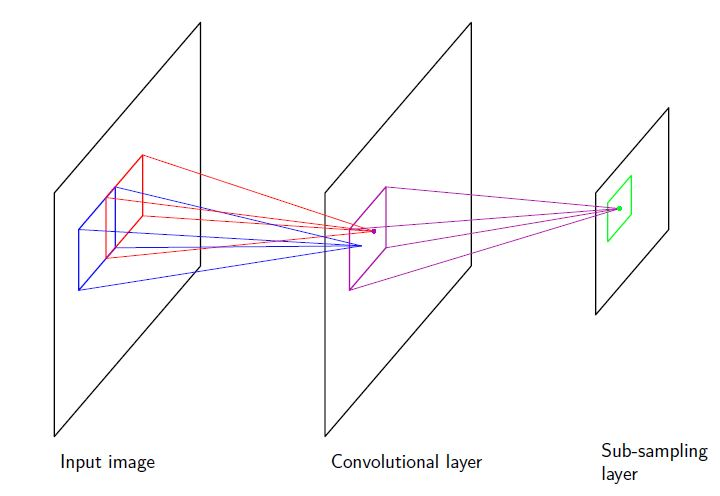
\includegraphics[scale = 0.5]{CNN0}
	\caption{Structure of CNN (1)}\label{CNN1}
\end{figure}
\begin{figure}
	\centering
	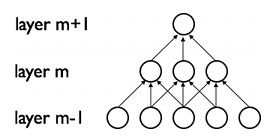
\includegraphics[scale = 0.5]{CNN}
	\caption{Structure of CNN (2)}\label{CNN2}
\end{figure}

In the convolutional layer the units are organized into planes each of which is called a \imp{feature map}, as illustrated in Figure \ref{CNN3}. 
\begin{figure}
	\centering
	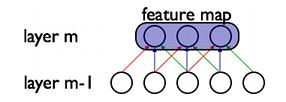
\includegraphics[scale = 0.5]{CNN2}
	\caption{Feature map}\label{CNN3}
\end{figure}
Units in a feature map each take inputs only from a \textbf{small subregion} of the region, and all of the units in a feature map are constrained to \textbf{share the same weight values}. Input values from a patch are linearly combined using the weights and the bias, and the result transformed by a sigmoidal nonlinearity. If we think of the units as feature detectors, then all of the units in a feature map detect the \textbf{same pattern} but at different locations in the input image. If the input image is shifted, the activations of the feature map will be shifted by the same amount. This provides the basis for the (\textbf{approximate}) invariance of the network outputs to translations and distortions of the input image.

The outputs of the convolutional units form the inputs to the subsampling layer of the network. For each feature map in the convolutional layer, there is a plane of units in the subsampling layer and each unit takes inputs from a small receptive field in the corresponding feature map. This sub-sampling layer is useful for adaptations.
\subsection{Mixture density networks}
\subsubsection{Model}
In order to model multimodal distributions, we can use a mixture model for $p(\bf{t|x})$ in which both the mixing coefficients as well as the component densities are flexible functions of the input vector $\bf{x}$, giving rise to the \imp{mixture density network}.

Here we develop the model explicitly for Gaussian components, so that
\begin{equation}
	p(\bf{t|x}) = \sum_{k=1}^K \pi_k(\bf{x}) \cal{N}(\bf{t}|\bs{\mu}_k(\bf{x}),\sigma_k^2(\bf{x}))
\end{equation}
This is an example of a \imp{heteroscedastic} model since the noise variance on the data is a function of the input vector $\bf{x}$.

The likelihood is given by
\begin{equation}
	E(\bf{w})= - \sum_{n=1}^N \ln \left\{ \sum_{k=1}^k \pi_k(\bf{x}_n,\bf{w})\cal{N}(\bf{t}_n|\bs{\mu}_k(\bf{x}_n,\bf{w}),\sigma_k^2(\bf{x}_n,\bf{w})) \right\}
\end{equation}

We now take the various parameters of the mixture model, namely the mixing coefficients $\pi_k(\bf{x})$, the means $\bs{\mu}_k(\bf{x})$, and the variances $\sigma_k^2(\bf{x})$, to be governed by the outputs of \textbf{one} conventional neural network that takes $\bf{x}$ as its input. 

The mixture density network is closely related to the mixture of \imp{experts}. The principle difference is that in the mixture density network the same function is used to predict the parameters of all of the component densities as well as the mixing coefficients, and so the nonlinear hidden units are \textbf{shared} amongst the input-dependent functions.
\subsubsection{Optimization}
We need to evaluate the derivatives of the error $E(\bf{w})$ with respect to the components of $\bf{w}$. These can be evaluated by using the standard backpropagation procedure, provided we obtain suitable expressions for the derivatives of the error with respect to the output-unit activations.

For convenience, we view the mixing coefficients $\pi_k(\bf{x})$ as $\bf{x}$-dependent prior probabilities and to introduce the corresponding posterior probabilities given by
\begin{equation}
	\gamma_{nk} = \gamma_k(\bf{t}_n|\bf{x}_n) = \frac{\pi_k \cal{N}_{nk}}{\sum_{l=1}^K \pi_l \cal{N}_{nl}}
\end{equation}

The derivatives with respect to the network output activations governing the mixing coefficients are given by
\begin{align}
	\frac{\partial E_n}{\partial a_{k}^{\pi}} &= \pi_k - \gamma_{nk} \\
	\frac{\partial E_n}{\partial a_{kl}^{\mu}} &= \gamma_{nk} \left\{ \frac{\mu_{kl}-t_{nl}}{\sigma_k^2} \right\} \\
	\frac{\partial E_n}{\partial a_{k}^{\sigma}} &= \gamma_{nk} \left\{ L - \frac{||\bf{t}_n-\bs{\mu}_k||^2}{\sigma_k^2} \right\}
\end{align}

\subsection{Bayesian neural networks}
Regularized maximum likelihood can be interpreted as a MAP approach in which the regularizer can be viewed as the logarithm of a prior parameter distribution.

\subsubsection{Posterior parameter distribution}
\begin{align}
	p(\cal{D}|\bf{w},\beta) &= \prod_{n=1}^N \cal{N}(t_n|y(\bf{x}_n,\bf{w}),\beta^{-1}) \\
	p(\bf{w}|\cal{D},\alpha,\beta) &\simeq p(\bf{w}|\alpha) p(\cal{D}|\bf{w},\beta) \\
	\ln p(\bf{w}|\cal{D}) &= -\frac{\alpha}{2} \bf{w}^{\intercal} \bf{w} - \frac{\beta}{2} \sum_{n=1}^N \{ y(\bf{x}_n,\bf{w})-t_n \}^2 + \up{const}.
\end{align}
This is non-Gaussian because of the nonlinear dependence of $y(\bf{x},\bf{w})$ on $\bf{w}$.

\subsubsection{Approximation}
We can find a Gaussian approximation to the posterior distribution by using the Laplace approximation. Having found a mode $\bf{w}_{MAP}$, we can then build a local Gaussian approximation by evaluating the matrix of second derivatives of the negative log posterior distribution. This is given by
\begin{equation}
	\bf{A} = -\nabla\nabla \ln p(\bf{w}_{MAP}|\cal{D},\alpha,\beta) = \alpha \bf{I} + \beta \bf{H}
\end{equation}
where $\bf{H}$ is the Hessian matrix comprising the second derivatives of the sum-of-squares error function with respect to the components of $\bf{w}$. We then get the corresponding Gaussian approximation to the posterior
\begin{equation}
	q(\bf{w}|\cal{D}) = \cal{N}(\bf{w}|\bf{w}_{MAP},\bf{A}^{-1}).
\end{equation}

Similarly, the predictive distribution is obtained by marginalizing with respect to this posterior distribution
\begin{equation}
	p(t|\bf{x},\cal{D}) = \int p(t|\bf{x,w})q(\bf{w}|\cal{D}) \ud \bf{w}.
\end{equation}
In order to make this integration analytically tractable, we assume that the posterior distribution has small variance compared with the characteristic scales of $\bf{w}$ over which $y(\bf{x,w})$ is varying. This allows us to make a Taylor expansion of the network function around $\bf{w}_{MAP}$ and retain only the linear terms
\begin{equation}
	y(\bf{x,w}) \simeq y(\bf{x},\bf{w}_{MAP}) + \bf{g}^{\intercal} (\bf{w}-\bf{w}_{MAP}).
\end{equation}
so that
\begin{equation}
	p(t|\bf{x,w},\beta) \simeq \cal{N}(t|y(\bf{x,w}_{MAP})+\bf{g}^{\intercal} (\bf{w-w}_{MAP}),\beta^{-1}).
\end{equation}
We can therefore use the formula for linear-Gaussian model to obtain
\begin{equation}
	p(t|\bf{x},\cal{D},\alpha,\beta) = \cal{N}(t|y(\bf{x},\bf{w}_{MAP}),\sigma^2(\bf{x}))
\end{equation}
where the input-dependent variance is given by
\begin{equation}
	\sigma^2(\bf{x}) = \beta^{-1} + \bf{g}^{\intercal} \bf{A}^{-1}\bf{g}.
\end{equation}
\subsubsection{Hyperparameter optimization}
The evidence for the hyperparameters is obtained by
\begin{equation}
	p(\cal{D}|\alpha,\beta) = \int p(\cal{D}|\bf{w},\beta)p(\bf{w}|\alpha) \ud \bf{w}.
\end{equation}
The function integrated is proportional to the posterior, which has been optimized. Directly apply (\ref{LapInt}), we obtain
\begin{equation}
	\ln p(\cal{D}|\alpha,\beta) \simeq -E(\bf{w}_{MAP}) - \frac{1}{2} \ln |\bf{A}| + \frac{W}{2}\ln \alpha + \frac{N}{2} \ln \beta -\frac{N}{2} \ln(2\pi)
\end{equation}
where $W$ is the total number of parameters in $\bf{w}$, and the regularized error function is defined by
\begin{equation}
	E(\bf{w}_{MAP}) = \frac{\beta}{2} \sum_{n=1}^N \{ y(\bf{x}_n,\bf{w}_{MAP})-t_n \}^2 + \frac{\alpha}{2}\bf{w}_{MAP}^{\intercal} \bf{w}_{MAP}.
\end{equation}

In the evidence framework, we make \textbf{point estimates} for $\alpha$ and $\beta$ by \textbf{maximizing} $\ln p(\cal{D}|\alpha,\beta)$. In order to handle derivatives of $\ln |\bf{A}|$ with respect to $\alpha$ and $\beta$, we define
\begin{equation}
	\beta \bf{H} \bf{u}_i = \lambda_i \bf{u}_i
\end{equation}
All others can be handled similarly to what we did in Section \ref{DEigens}.

The Bayesian neural networks for classification can be handled similarly but with bullshit mathematical manipulations.
\section{Kernel Methods}
There are \imp{memory-based} methods that involve storing the entire training set in order to make predictions for future data points, other than discarding them when making predictions. These methods are usually fast to train but slow at making predictions for test data points.

The kernel function is defined as
\begin{equation}
	k(\bf{x,x'}) = \bs{\phi}(\bf{x}^{\intercal}) \bs{\phi}(\bf{x'})
\end{equation}

The ideology of kernel methods is that we replace the basis feature functions with kernels which are inner product of them so as to evade some disadvantages of them. In other words, we can work directly in terms of kernels and avoid the explicit introduction of the feature vector $\bs{\phi}(\bf{x})$, which allows us implicitly to use feature spaces of \textbf{high, even infinite, dimensionality}. Many algorithms can be represented in a dual form by kernels.

\subsection{Properties of kernels}
The Gram matrix $\bf{K}$ is defined as
\begin{equation}
	K_{nm} = \bs{\phi}(\bf{x}_n)^{\intercal} \bs{\phi}(\bf{x}_m) = k(\bf{x}_n,\bf{x}_m)
\end{equation}
What's more, a \textbf{necessary and sufficient} condition for a function $k(\bf{x,x'})$ to be a valid kernel is that the Gram matrix $\bf{K}$, whose elements are given by $k(\bf{x}_n,\bf{x}_m)$, should be \textbf{positive semidefinite} for \textbf{all possible} choices of the set $\{ \bf{x}_n \}$.

One powerful technique for constructing new kernels is to build them out of simpler kernels as building blocks. This can be done using the following properties, given valid kernels $k_1(\bf{x,x'})$ and $k_2(\bf{x,x'})$:
\begin{align}
	k(\bf{x,x'}) &= ck_1(\bf{x,x'}) \\
	k(\bf{x,x'}) &= f(\bf{x})k_1(\bf{x,x'})f(\bf{x'})\\
	k(\bf{x,x'}) &= q(k_1(\bf{x,x'}))\\
	k(\bf{x,x'}) &= \exp (k_1(\bf{x,x'}))\\
	k(\bf{x,x'}) &=k_1(\bf{x,x'})+k_2(\bf{x,x'})\\
	k(\bf{x,x'}) &=k_1(\bf{x,x'})k_2(\bf{x,x'})\\
	k(\bf{x,x'}) &=k_3(\bs{\phi}(\bf{x}),\bs{\phi}(\bf{x'}))\\
	k(\bf{x,x'}) &=\bf{x}^{\intercal} \bf{Ax'}\\
	k(\bf{x,x'}) &=k_a (\bf{x}_a,\bf{x}_a')+k_b(\bf{x}_b,\bf{x}_b')\\
	k(\bf{x,x'}) &=k_a (\bf{x}_a,\bf{x}_a')k_b(\bf{x}_b,\bf{x}_b')
\end{align}
where $c > 0$ is a constant, $f(\cdot)$ is any function, $q(\cdot)$ is a polynomial with nonnegative coefficients, $\bs{\phi}(\bf{x})$ is a function from $\bf{x}$ to $\bb{R}^M$, $k_3(\cdot,\cdot)$ is a valid kernel in $\bb{R}^M$, $\bf{A}$ is a symmetric positive semidefinite matrix, $\bf{x}_a$ and $\bf{x}_b$ are variables (not necessarily disjoint) with $\bf{x} = (\bf{x}_a, \bf{x}_b)$, and $k_a$ and $k_b$ are valid kernel functions over their respective spaces.

\subsection{Gaussian processes}
\subsubsection{Motivation}
The predictions of linear regression can be reformulated as
\begin{equation}
	\bf{y } = \bs{\Phi} \bf{w}
\end{equation}
where $\bs{\Phi}$ is the design matrix. Since $\bf{w}$ has a Gaussian prior $p(\bf{w}) = \cal{N}(\bf{w}|\bf{0},\alpha^{-1}\bf{I})$, $\bf{y}$ is itself Gaussian, whose mean and covariance are given by
\begin{align}
	\bb{E}[\bf{y}] &= \bs{\Phi} \bb{E}[\bf{w}] = 0\\
	\up{cov}[\bf{y}] &= \bb{E}[\bf{y}\bf{y}^{\intercal}] = \bs{\Phi}\bb{E}[\bf{w}\bf{w}^{\intercal}]\bs{\Phi}^{\intercal} = \frac{1}{\alpha}\bs{\Phi}\bs{\Phi}^{\intercal} = \bf{K}.
\end{align}
where $K$ is the Gram matrix with elements
\begin{equation}
	K_{nm} = k(\bf{x}_n,\bf{x}_m) = \frac{1}{\alpha} \bs{\phi}(\bf{x}_n)^{\intercal} \bs{\phi}(\bf{x}_m).
\end{equation}

The fact that $\{ y_n \}$ forms a Gaussian processes mean we can choose the mean and covariance to completely specify the process. By symmetry we choose $\bb{E}[\bf{y}] = \bf{0}$. The covariance is chosen to be the Gram matrix of some user-specified kernels, i.e. $\bb{E}[y(\bf{x}_n) y(\bf{x}_m)]=k(\bf{x}_n,\bf{x}_m)$, such as the exponential kernel leading to the \imp{Ornstein-Uhlenbeck} process.
\subsubsection{Linear regression}
The model is given by
\begin{equation}
	p(\bf{t|y}) = \cal{N}(\bf{t|y},\beta^{-1} \bf{I}_N)
\end{equation}
where $\bf{y}$ serves as an latent variable and its prior is given by
\begin{equation}
	p(\bf{y}) = \cal{N}(\bf{y|0,K}).
\end{equation}
The marginal distribution $p(\bf{t})$ is obtained by integrating out the latent variable $\bf{y}$:
\begin{equation}
	p(\bf{t}) = \int p(\bf{t|y})p(\bf{y}) \ud \bf{y} = \cal{N}(\bf{t}|\bf{0,C})
\end{equation}
where
\begin{equation}
	C(\bf{x}_n,\bf{x}_m) = k(\bf{x}_n,\bf{x}_m) + \beta^{-1} \delta_{nm}. \label{GauPro1}
\end{equation}

In order to derive the predictive distribution $p(t_{N+1}|\bf{t}_N)$, where we have left the \textbf{conditioning} on the input variables \textbf{implicit}, we first derive the joint distribution $p(\bf{t}_{N+1})$:
\begin{equation}
	p(\bf{t}_{N+1}) = \cal{N}(\bf{t}_{N+1}|\bf{0,C}_{N+1})
\end{equation}
where
\begin{equation}
	\bf{C}_{N+1} = \begin{pmatrix}
	 \bf{C}_N & \bf{k} \\
	 \bf{k}^{\intercal} & c
	\end{pmatrix}.
\end{equation}
where $\bf{C}_N$ is the covariance matrix with elements given by (\ref{GauPro1}). For $n,m=1,\cdots,N$, the vector $\bf{k}$ has elements $k(\bf{x}_n,\bf{x}_{N+1})$ for $n=1,\cdots,N$, and the scalar $c=k(\bf{x}_{N+1},\bf{x}_{N+1})+\beta^{-1}$. As a result, the conditional distribution $p(t_{N+1}|\bf{t}_N)$ can be derived readily, given by
\begin{align}
	m(\bf{x}_{N+1}) &= \bf{k}^{\intercal} \bf{C}_N^{-1} \bf{t} \\
	\sigma^2(\bf{x}_{N+1}) &= c - \bf{k}^{\intercal} \bf{C}_N^{-1} \bf{k}.\label{GauPreVar}
\end{align}

The viewpoint of Gaussian processes has greater advantages in \textbf{high-dimensional} cases where $p >> N$.

\textbf{Hyperparameters and automatic relevance determination}. The kernels may have parameters, for example, to control the length scale of the correlations. As a result, these parameters belong to the model hyperparameters. The simplest approach is to make a point estimate of $\bs{\theta}$ by maximizing the log likelihood function
\begin{equation}
 \ln p(\bf{t}|\bs{\theta}) = -\frac{1}{2} \ln |\bf{C}_N| - \frac{1}{2} \bf{t}^{\intercal} \bf{C}_N^{-1} \bf{t} - \frac{N}{2} \ln (2\pi).
\end{equation}
and the gradient with respect to the parameters are
\begin{equation}
	\frac{\partial }{\partial \theta_i} \ln p(\bf{t}|\bs{\theta}) = -\frac{1}{2}\up{Tr}\left( \bf{C}_N^{-1} \frac{\partial \bf{C}_N}{\partial \theta_i} \right) + \frac{1}{2} \bf{t}^{\intercal} \bf{C}_N^{-1} \frac{\partial \bf{C}_N}{\partial \theta_i}\bf{C}_N^{-1} \bf{t}.
\end{equation}

With parameters corresponding to different terms in the kernel function, we can determine their relative importance. This leads to the technique of \imp{automatic relevance determination} (ARD), where we incorporate a separate parameter for each dimensionality of the input variables and then infer these parameters from the data.
\subsubsection{Linear classification}
We first introduce the latent variable $\bf{a}_{N+1}$, which denotes the mean of Bernoulli distributions for every point:
\begin{equation}
	p(\bf{a}_{N+1}) = \cal{N}(\bf{a}_{N+1}|\bf{0,C}_{N+1})
\end{equation}
where the covariance matrix $\bf{C}_{N+1}$ has elements given by
\begin{equation}
	C(\bf{x}_n,\bf{x}_m) = k(\bf{x}_n,\bf{x}_m) + \nu \delta_{nm}.
\end{equation}
Here the extra term $\nu \delta_{nm}$ is introduced to \textbf{ensure the validity of covariance}. In contrast to regression case, we introduce this term explicitly here because the prior for $\bf{a}_{N+1}$ will be \textbf{directly} used to make predictions while this is not necessary in regression since the final predictive distribution is OK.

The required predictive distribution is given by
\begin{align}
	p(t_{N+1} = 1|\bf{t}_N) &= \int p(t_{N+1} = 1|a_{N+1})p(a_{N+1}|\bf{t}_N) \ud a_{N+1}\\
	&=  \int \sigma(a_{N+1}) p(a_{N+1}|\bf{t}_N) \ud a_{N+1}
\end{align}
Since this integral is analytical intractable, there are four approaches to obtain an approximate solution:
\begin{itemize}
	\item Sampling methods.
	\item Laplace approximation.
	\item Variational inference.
	\item Expectation propagation. Since the true posterior is unimodal.
\end{itemize}

\textbf{Laplace approximation}. First, we have
\begin{equation}
	p(a_{N+1}|\bf{t}_N) = \int p(a_{N+1}|\bf{a}_N)p(\bf{a}_N|\bf{t}_N) \ud \bf{a}_N
\end{equation}
The conditional distribution $p(a_{N+1}|\bf{a}_N)$ is easy to obtain, given by
\begin{equation}
	p(a_{N+1}|\bf{a}_N) = \cal{N}(a_{N+1}|\bf{k}^{\intercal} \bf{C}_N^{-1}\bf{a}_N, c-\bf{k}^{\intercal}\bf{C}_N^{-1}\bf{k}).
\end{equation}

The posterior distribution is evaluated using Bayesian formula. First, we know the prior $p(\bf{a}_{N+1})$. Second, we have
\begin{equation}
	p(\bf{t}_N|\bf{a}_N) = \prod_{n=1}^N \sigma(a_n)^{t_n} (1-\sigma(a_n))^{1-t_n} = \prod_{n=1}^N e^{a_n t_n}\sigma(-a_n).
\end{equation}
Then we get the log posterior distribution:
\begin{align}
	\Psi(\bf{a}_N) &= \ln p(\bf{a}_N) + \ln p(\bf{t}_N|\bf{a}_N) \\
	&= -\frac{1}{2} \bf{a}_N^{\intercal} \bf{C}_N^{-1} \bf{a}_N - \frac{N}{2} \ln (2\pi) - \frac{1}{2} \ln |\bf{C}_N| + \bf{t}_N^{\intercal}\bf{a}_N \\
	&\quad  -\sum_{n=1}^N \ln (1+e^{a_n}).
\end{align}

Next we need to find the mode of the posterior distribution, and this requires the gradient and Hessian of $\Psi(\bf{a}_N)$:
\begin{align}
	\nabla \Psi(\bf{a}_N) &= \bf{t}_N - \bs{\sigma}_N - \bf{C}_N^{-1} \bf{a}_N \\
    \bf{H} = -\nabla\nabla \Psi(\bf{a}_N) &=  \bf{W}_N + \bf{C}_N^{-1}
\end{align}
where $\bf{W}_N$ is a diagonal matrix with elements $\sigma(a_n)(1-\sigma(a_n))$.

Then we can employ the Newton-Raphson formula to get the optimal parameters $\bf{a}_N$ and its corresponding Hessian. The Gaussian approximation to the posterior distribution
\begin{equation}
	q(\bf{a}_N) = \cal{N}(\bf{a}_N|\bf{a}_N^*,\bf{H}^{-1})
\end{equation}

Afterwards, we know that $p(\bf{a}_N|\bf{t}_N)$ is a Gaussian distribution with the parameters given by
\begin{align}
	\bb{E}[a_{N+1}|\bf{t}_N] &= \bf{k}^{\intercal} (\bf{t}_N - \bs{\sigma}_N) \\
	\up{var}[a_{N+1}|\bf{t}_N] &= c - \bf{k}^{\intercal} (\bf{W}_N^{-1}+\bf{C}_N)^{-1} \bf{k}.
\end{align}

Finally, we can approximate the predictive distribution and the model evidence based on the results above.

\subsubsection{Connection to neural networks}
In a Bayesian prospective, it makes little sense to limit the number of parameters in the network according to the size of the training set since there is no over-fitting there.

In a Bayesian neural network, the prior distribution over the parameter vector $\bf{w}$, in conjunction with the network function $f(\bf{x,w})$, produces a prior distribution over functions from $y(\bf{x})$ where $\bf{y}$ is the vector of network outputs. Neal (1996) has shown that, for a broad class of prior distributions over $\bf{w}$, the distribution of functions generated by a neural network will tend to a Gaussian process in the limit $M \rightarrow \infty$.

\subsection{SVM}
SVM is not a probabilistic model, and its model hyperparameters should be found using a hold out method such as \imp{cross-validation}.
\subsubsection{Classification}
The basic idea behind SVM for classification tasks is to find a hyperplane in feature space so that the distance of the closest point to the plane is largest. In case some data sets are not linear separable and to make the model more flexible, we introduce special variables called \imp{slack variables} to ``soften'' the original hard margin requirement. 

The hyperplane is defined by
\begin{equation}
	y(\bf{w}) = \bf{w}^{\intercal} \bs{\phi}(\bf{x}) + b.
\end{equation}

After introducing these slack variables, the constraints are replaced by
\begin{equation}
	t_n y(\bf{x}_n) \geq 1 -\xi_n \qquad n = 1,\cdots,N
\end{equation}
in which the slack variables are constrained to satisfy $\xi_n \geq 0$.

We omit some intuitions from geometry. Our goal is now to maximize the margin while softly penalizing points that lie on the wrong side of the margin boundary. We therefore minimize
\begin{equation}
	C\sum_{n=1}^N \xi_n + \frac{1}{2} ||\bf{w}||^2
\end{equation}
where the parameter $C > 0$ controls the trade-off between the slack variable penalty and the margin.

We now employ the Lagrange multipliers to give the Lagrangian
\begin{equation}
	L(\bf{w},b,\bf{a},\bs{\xi},\bs{\mu}) = \frac{1}{2} ||\bf{w}||^2 + C \sum_{n=1}^N \xi_n - \sum_{n=1}^N a_n \{ t_n y(\bf{x}_n) -1 + \xi_n \} - \sum_{n=1}^N \mu_n \xi_n.
\end{equation}
The corresponding set of KKT conditions are given by
\begin{align}
	a_n &\geq 0 \\
	t_n y(\bf{x}_n) -1 + \xi_n &\geq 0 \\
	a_n(t_n y(\bf{x}_n)-1+\xi_n) &= 0 \\
	\mu_n &\geq 0 \\
	\xi_n & \geq 0 \\
	\mu_n \xi_n &= 0
\end{align}
when $n = 1,\cdots,N$.

We now optimize out $\bf{w}$, $b$ and $\{\xi_n\}$ making use of the definition of $y(\bf{x})$ to give
\begin{align}
	\frac{\partial L}{\partial \bf{w}} &= 0 \quad \Rightarrow \quad \bf{w} = \sum_{n=1}^N a_n t_n \bs{\phi}(\bf{x}_n) \\
	\frac{\partial L}{\partial b} &= 0 \quad \Rightarrow \quad \sum_{n=1}^N a_n t_n = 0\\
	\frac{\partial L}{\partial \xi_n} &= 0  \quad \Rightarrow \quad a_n = C -\mu_n.
\end{align}
Using these results to eliminate $\bf{w}$, $b$ and $\{\xi_n\}$ from the Lagrangian, we obtain the dual Lagrangian in the form
\begin{equation}
	\tilde{L}(\bf{a}) = \sum_{n=1}^N a_n -\frac{1}{2} \sum_{n=1}^N \sum_{m=1}^N a_n a_m t_n t_m k(\bf{x}_n,\bf{x}_m).
\end{equation}
This is an identity completely comprised of Lagrangian multipliers, which is identical to the separable case, except that the constraints are different:
\begin{align}
	0 \leq a_n \leq C \\
	\sum_{n=1}^N a_n t_n = 0
\end{align}
The resulting marginal classifier can be written as
\begin{equation}
	y(\bf{x}) = \sum_{n=1}^N a_n t_n k(\bf{x,x}_n) + b
\end{equation}
From which we assert that data points with $a_n = 0$ play no role in making predictions and hence the remaining data points are called \imp{support vectors}.

The SVM can be trained using the SMO algorithm, as discussed in Section \ref{SMO}. Having found $\bf{a}$, we then determine the value of the threshold parameter $b$ by noting that any support vector $\bf{x}_n$ satisfies $t_ny(\bf{x}_n) = 1$, which gives
\begin{equation}
	b = \frac{1}{N_{\cal{S}}} \sum_{n \in \cal{S}} \left( t_n - \sum_{m \in \cal{S}} a_m t_m k(\bf{x}_n,\bf{x}_m) \right)
\end{equation}

The SVM is fundamentally a two-class classifier. The most commonly used method to handle multi-class tasks is to adopt the \imp{one-versus-the-rest} approach despite its abundant disadvantages.

\subsubsection{Regression}
The basic idea behind SVM for regression tasks is to find a hyperplane as simple as possible in feature space so that all training points lie in an $\epsilon$-tube around the plane. However, this is impossible for some data sets so again \imp{slack variables} are need to soften the hard margin requirement.

The conditions are
\begin{align}
	t_n &\leq y(\bf{x}_n) + \epsilon + \xi_n \\
	t_n &\geq y(\bf{x}_n) - \epsilon - \hat{\xi}_n
\end{align}
and the error function for support vector regression can then be written as
\begin{equation}
	C \sum_{n=1}^{N}(\xi_n + \hat{\xi}_n) + \frac{1}{2} ||\bf{w}||^2.
\end{equation}
We introduce the Lagrangian
\begin{align}
	L = & C \sum_{n=1}^N (\xi_n + \hat{\xi}_n) + \frac{1}{2} ||\bf{w}||^2 - \sum_{n=1}^N (\mu_n\xi_n + \hat{\mu}_n\hat{\xi}_n) \\
	 &- \sum_{n=1}^N a_n(\epsilon + \xi_n + y_n -t_n) - \sum_{n=1}^N \hat{a}_n(\epsilon+\hat{\xi}_n-y_n+t_n).
\end{align}
Then we set the derivatives of the Lagrangian with respect to $\bf{w}$, $b$, $\xi_n$, and $\hat{\xi}_n$ to zero, giving
\begin{align}
	\frac{\partial L}{\partial \bf{w}} &= 0 \quad \Rightarrow \quad \bf{w} = \sum_{n=1}^N (a_n-\hat{a}_n)\bs{\phi}(\bf{x}_n)\\
	\frac{\partial L}{\partial b} &=0 \quad \Rightarrow \quad \sum_{n=1}^N(a_n-\hat{a}_n) = 0 \\
	\frac{\partial L}{\partial \xi_n} &= 0 \quad \Rightarrow \quad a_n+\mu_n = C \\
	\frac{\partial L}{\partial \hat{\xi}_n} &= 0 \quad \Rightarrow \quad \hat{a}_n+\hat{\mu}_n = C.
\end{align}
Using these results to simplify the Lagrangian, we obtain
\begin{align}
	\tilde{L}(\bf{a},\hat{\bf{a}}) = &-\frac{1}{2} \sum_{n=1}^N \sum_{m=1}^N (a_n-\hat{a}_n)(a_m-\hat{a}_m)k(\bf{x}_n,\bf{x}_m) \\
	&- \epsilon \sum_{n=1}^N (a_n+\hat{a}_n) + \sum_{n=1}^N (a_n - \hat{a}_n)t_n
\end{align}
and again we have the box constraints
\begin{align}
	0 \leq a_n &\leq C \\
	0 \leq \hat{a}_n &\leq C \\
	\sum_{n=1}^N (a_n - \hat{a}_n) &= 0.
\end{align}
The corresponding KKT conditions are given by
\begin{align}
	a_n(\epsilon + \xi_n + y_n -t_n) &= 0\\
	\hat{a}_n(\epsilon + \hat{\xi}_n-y_n+t_n) &= 0\\
	(C - a_n)\xi_n &= 0\\
	(C - \hat{a}_n) \hat{\xi}_n &= 0.
\end{align}
The predictions are given by
\begin{equation}
	y(\bf{x}) = \sum_{n=1}^N (a_n - \hat{a}_n)k(\bf{x},\bf{x}_n) +b.
\end{equation}
The solution can be found by a similar algorithm to SMO. From the KKT conditions we again know that for every data point $\bf{x}_n$, either $a_n$ or $\hat{a}_n $ (or \textbf{both}) must be zero. As a result, we again have a sparse solution.
\subsection{RVM}
RVM is a probabilistic counterpart of SVM. 
\subsubsection{Regression}
The predictive conditional distribution is the same in liner regression model. However, the basis functions are specialized to kernel forms and the prior of $\bf{w}$ is changed to an \textbf{ARD prior}:
\begin{align}
	y(\bf{x}) &= \sum_{n=1}^{N} w_n k(\bf{x},\bf{x}_n) + b\\
	p(\bf{w}|\bs{\alpha}) &= \prod_{i=1}^M \cal{N}(w_i |0,\alpha_i^{-1})
\end{align}

The followings are similar to what has been discussed in Section \ref{LMR} with only minor modifications, including evidence approximation and predictive distribution. In the case of evidence maximization, EM is found in practice to be slower than direct iteration methods. A better algorithm for training $\{ \alpha_i\}$ is the \imp{sequential sparse Bayesian learning algorithm}, which is discussed in Section \ref{SSBL}. 

An important drawback for RVM results from its \textbf{localized basis functions}. We can see from a similar result to (\ref{LRPreVar}) that the predictive variance for linear regression models becomes small in regions of input space where there are no basis functions, and the model will therefore become increasingly certain of its predictions when extrapolating outside the domain of the data. The predictive distribution in Gaussian process regression does not suffer from this problem, as we can see from (\ref{GauPreVar}). However, the computational cost of making predictions with a RVM is typically much lower than a Gaussian process because of sparsity.
\subsubsection{Classification}
We again introduce an ARD prior and the followings are similar to what we have discussed in Section \ref{LC}. The maximization of the evidence function, which is paramount for automatic relevance determination, is specified here.

We already have the parameters of the Laplace approximation to the posterior distribution of $\bf{w}$, given by
\begin{align}
	\bf{w}^* &= \bf{A}^{-1} \bs{\Phi}^{\intercal} (\bf{t-y}) \\
	\bs{\Sigma} &= (\bs{\Phi}^{\intercal} \bf{B} \bs{\Phi} + \bf{A})^{-1}
\end{align}
where $\bf{A} = \up{diag}(\alpha_i)$ and $\bf{B} = \up{diag}\{y_n(1-y_n)\}$. 

From (\ref{LCEvi}) we obtain
\begin{equation}
	p(\bf{t}|\alpha) \simeq p(\bf{t|w}^*)p(\bf{w}^*|\bs{\alpha})(2\pi)^{M/2}|\bs{\Sigma}|^{1/2}.
\end{equation}
Setting the derivatives of the marginal likelihood with respect to $\alpha_i$ to zero, we obtain
\begin{equation}
	-\frac{1}{2}(w_i^*)^2 + \frac{1}{2\alpha_i}-\frac{1}{2}\Sigma_{ii} = 0.
\end{equation}
Defining $\gamma_i = 1-\alpha_i \Sigma_{ii}$ and rearranging then gives
\begin{equation}
	\alpha_i^{new} = \frac{\gamma_i}{(w_i^*)^2}.
\end{equation}

If we define
\begin{equation}
	\hat{\bf{t}} = \bs{\Phi} \bf{w}^* + \bf{B}^{-1}(\bf{t-y})
\end{equation}
we can write the approximate log marginal likelihood in the form
\begin{equation}
	\ln p(\bf{t}|\bs{\alpha}) = -\frac{1}{2}\left\{ N \ln(2\pi) + \ln |\bf{C}| + (\hat{\bf{t}})^{\intercal} \bf{C}^{-1} \hat{\bf{t}} \right\}
\end{equation}
where
\begin{equation}
	\bf{C=B}+\bs{\Phi}\bf{A}\bs{\Phi}^{\intercal}.
\end{equation}
This takes the same form as the evidence function (\ref{RVMl}) in the regression case, and so we can apply the same analysis of \textbf{sparsity} and obtain the same fast learning algorithm in which we fully optimize a single hyperparameter $\alpha_i$ at each step.
\subsubsection{Conclusions}
The principal disadvantage of the RVM is the relative \textbf{long training times} compared with the SVM. This is offset, however, by the \textbf{avoidance of cross-validation} runs to set the model complexity parameters. Furthermore, because it yields \textbf{sparser} models, the computation time on test points, which is usually the more important consideration in practice, is typically much less.

\section{Mixture Models}
\subsection{Gaussian mixture model (GMM)}
This is a model used for unsupervised learning tasks like clustering.
\subsubsection{Model}
Gaussian mixture models are also called mixtures of Gaussians (MOG). It can be written as a linear superposition of Gaussians in the form
\begin{equation}
	p(\bf{x}) = \sum_{k=1}^K \pi_k \cal{N}(\bf{x}|\bs{\mu}_k,\bs{\Sigma}_k).
\end{equation}
We now introduce a $K$-dimensional binary random \textbf{latent} variable $\bf{z}$ having a \imp{1-of-$K$} representation in which a particular element $z_k$ is equal to 1 and all other elements are equal to 0. As a result
\begin{align}
 p(\bf{z}) &= \prod_{k=1}^{K} \pi_k^{z_k} \\
 p(\bf{x}|z_k=1) &= \cal{N}(\bf{x}|\bs{\mu}_k,\bs{\Sigma}_k) \\
 p(\bf{x|z})&= \prod_{k=1}^K \cal{N}(\bf{x}|\bs{\mu}_k,\bs{\Sigma}_k)^{z_k}\\
 p(\bf{x}) = \sum_{\bf{z}} p(\bf{z})p(&\bf{x|z}) = \sum_{k=1}^K \pi_k \cal{N}(\bf{x}|\bs{\mu}_k,\bs{\Sigma}_k).
\end{align}

In addition, we use $\gamma(z_k)$ to denote $p(z_k=1|\bf{x})$, whose value can be found using Bayes' theorem
\begin{align}
	\gamma(z_k)\equiv p(z_k=1|\bf{x}) &= \frac{p(z_k=1)p(\bf{x}|z_k=1)}{\sum_{j=1}^K p(z_j=1)p(\bf{x}|z_j=1)} \\
	&= \frac{\pi_k \cal{N}(\bf{x}|\bs{\mu}_k,\bs{\Sigma}_k)}{\sum_{j=1}^K \pi_j \cal{N}(\bf{x}|\bs{\mu}_j,\bs{\Sigma}_j)}.
\end{align}
$\gamma(z_k)$ can also be viewed as the \imp{responsibility} that component $k$ takes for ``explaining'' the observation $\bf{x}$.
\subsubsection{Likelihood}
The log of the likelihood function is given by
\begin{equation}
	\ln p(\bf{X}|\bs{\pi,\mu,\Sigma}) = \sum_{n=1}^N \ln \left\{ \sum_{k=1}^K \pi_k \cal{N}(\bf{x}_n|\bs{\mu}_k,\bs{\Sigma}_k) \right\}.
\end{equation}

There are two points to notice:
\begin{itemize}
\item The likelihood may have severe \textbf{singularities}, which will always happen whenever one of the Gaussian components ``\textbf{collapses}'' onto a specific data point. Suppose a Gaussian has the covariance matrix $\bs{\Sigma}_k = \sigma_k^2 \bf{I}$, and its mean $\bs{\mu}_j$ exactly equals to one of the data points so that $\bs{\mu}_j = \bf{x}_n$. The data point will then contribute a term in the likelihood of the form
\begin{equation}
	\cal{N}(\bf{x}_n|\bf{x}_n,\sigma_j^2 \bf{I}) = \frac{1}{(2\pi)^{1/2}}\frac{1}{\sigma_j}
\end{equation}
which will go to infinity in the limit $\sigma_j \rightarrow 0$. As a result, a likelihood having such singularities can never be optimized since it can be as large as it wishes to be. This is a unique phenomenon for \textbf{mixtures}. We need wipe out these singularities by using some heuristics, such as detecting when a Gaussian component is collapsing and resetting its mean to a randomly chosen value while also resetting its covariance to some large value.
\item In mixture models, a $K$-component mixture will have a total of $K!$ equivalent solutions corresponding to the $K!$ ways of assigning $K$ sets of parameters to $K$ components. This problem is called \imp{identifiability} and should be taken into account in the case of model comparison.
\end{itemize}
\subsubsection{EM for GMM}
The log joint distribution of the complete data is 
\begin{equation}
	\ln p(\bf{X,Z}|\bs{\mu,\Sigma,\pi}) = \sum_{n=1}^N \sum_{k=1}^K z_{nk}\{ \ln \pi_k +\ln \cal{N}(\bf{x}_n|\bs{\mu}_k,\bs{\Sigma}_k)\}
\end{equation}
Maximize this joint distribution with respect to $\pi_k$ directly by Lagrangian multipliers, we obtain
\begin{equation}
	\pi_k = \frac{1}{N} \sum_{n=1}^N z_{nk}.
\end{equation}

\textbf{The E step}. The expected value of the complete-data log likelihood function is therefore given by
\begin{equation}
	\bb{E}_{\bf{Z}}[\ln p(\bf{X,Z}|\bs{\mu,\Sigma,\pi})] = \sum_{n=1}^N \sum_{k=1}^K \bb{E}[z_{nk}]\{ \ln \pi_k + \ln \cal{N}(\bf{x}_n|\bs{\mu}_k,\bs{\Sigma}_k) \} \label{GMME}
\end{equation}
where the expected value of the posterior variable $z_{nk}$ under this posterior distribution is then given by
\begin{align}
	\bb{E}[z_{nk}] &= \frac{\sum_{\bf{z}_n} z_{nk}\prod_{k'}[ \pi_{k'} \cal{N}(\bf{x}_n|\bs{\mu}_{k'},\bs{\Sigma}_{k'})]^{z_{nk'}}}{\sum_{\bf{z}_n}\prod_j[\pi_j \cal{N}(\bf{x}_n|\bs{\mu}_j,\bs{\Sigma}_j)]^{z_{nj}}} \\
	&= \frac{\pi_k \cal{N}(\bf{x}_n|\bs{\mu}_k,\bs{\Sigma}_k)}{\sum_{j=1}^K \pi_j \cal{N}(\bf{x}_n|\bs{\mu}_j,\bs{\Sigma}_j)}=\gamma(z_{nk})
\end{align}

\textbf{The M step}. Maximize (\ref{GMME}) directly with respect to $\bs{\mu}_k$, $\bs{\Sigma}_k$ and $\pi_k$ leads to closed form solutions given by
\begin{align}
	\bs{\mu}_k^{new} &= \frac{1}{N_k} \sum_{n=1}^N \gamma(z_{nk})\bf{x}_n \\
	\bs{\Sigma}_k^{new} &= \frac{1}{N_k} \sum_{n=1}^N \gamma(z_{nk}) (\bf{x}_n - \bs{\mu}_k)(\bf{x}_n-\bs{\mu}_k)^{\intercal} \\
	\pi_k^{new} &= \frac{N_k}{N}.
\end{align}
\subsection{$K$-means}
$K$-means can be viewed as a special case of the \textbf{EM} algorithm for GMM, in which the covariance matrices of the mixture components share $\epsilon\bf{I}$ and $\epsilon$ is treated as a fixed constant instead of a parameter to be re-estimated and $\epsilon \rightarrow 0$. 

Intuitively, we define an objective function called a \imp{distortion measure}, given by
\begin{equation}
	J = \sum_{n=1}^N \sum_{k=1}^K r_{nk} || \bf{x}_n - \bs{\mu}_n||^2
\end{equation}
Then we optimize with respect to $r_{nk}$ and $\bs{\mu}_k$ alternatively, which leads to the $K$-means algorithm.

$K$-means can serve as a pretreatment for more complex algorithms like GMM.
\subsection{Mixtures of Bernoulli distributions}
This model is also known as \imp{latent class analysis}. We make the naive Bayes assumption and give the proposal distribution
\begin{equation}
	p(\bf{x}|\bs{\mu}) = \prod_{i=1}^D \mu_i^{x_i}(1-\mu_i)^{(1-x_i)}
\end{equation}

Now let us consider a finite mixture of these distributions given by
\begin{equation}
	p(\bf{x}|\bs{\mu,\pi}) = \sum_{k=1}^K \pi_k p(\bf{x}|\bs{\mu}_k).
\end{equation}

The log likelihood function for this model is given by
\begin{equation}
	\ln p(\bf{X}|\bs{\mu,\pi}) = \sum_{n=1}^N \ln \left\{ \sum_{k=1}^K \pi_k p(\bf{x}_n|\bs{\mu}_k) \right\}.
\end{equation}

Then we introduce the latent variable $\bf{z}$, as
\begin{equation}
	p(\bf{x|z},\bs{\mu}) = \prod_{k=1}^K p(\bf{x}|\bs{\mu}_k)^{z_k}
\end{equation}
while the prior distribution for the latent variables is given by
\begin{equation}
	p(\bf{z}|\bs{\pi}) = \prod_{k=1}^K \pi_k^{z_k}.
\end{equation}

Hereby we invoke the EM algorithm. The complete-data log likelihood function is given by
\begin{align}
	\ln p(\bf{X,Z}|\bs{\mu,\pi}) = \sum_{n=1}^{N} \sum_{k=1}^K z_{nk}  \left\{   \ln \pi_k 
	+ \sum_{i=1}^D [ x_{ni}\ln \mu_{ki}+(1-x_{ni})\ln(1-\mu_{ki}) ]  \right\} 
\end{align}

\textbf{The E step}. We take the expectation of the complete-data log likelihood with respect to the posterior distribution of the latent variables to give
\begin{equation}
	\bb{E}_{\bf{Z}}[\ln p(\bf{X,Z}|\bs{\mu,\pi})]=\sum_{n=1}^{N}\sum_{k=1}^K \gamma(z_{nk})\left\{\ln \pi_k + \sum_{i=1}^D [x_{ni}\ln \mu_{ki}+(1-x_{ni})\ln(1-\mu_{ki})] \right\}\label{BMME}
\end{equation}
where
\begin{align}
	\gamma(z_{nk}) =  \bb{E}[z_{nk}] = \frac{\pi_k p(\bf{x}_n|\bs{\mu}_k)}{\sum_{j=1}^K \pi_j p(\bf{x}_n|\bs{\mu}_j)}.
\end{align}

\textbf{The M step}. Setting the derivative of (\ref{BMME}) with respect to $\bs{\mu}_k$ equal to zero and rearrange the terms, we obtain
\begin{equation}
	\bs{\mu}_k = \bar{\bf{x}}_k = \frac{1}{N_k}\sum_{n=1}^N \gamma(z_{nk}) \bf{x}_n.
\end{equation}
For the maximization with respect to $\pi_k$,we need to introduce a Lagrange multiplier to enforce the constraint $\sum_k \pi_k = 1$ and we then obtain
\begin{equation}
	\pi_k = \frac{N_k}{N} = \frac{\sum_{n=1}^N \gamma(z_{nk})}{N}.
\end{equation}
\subsection{Bagging}
We want to find a way to introduce variability between the different models within the committee. One approach is to use \imp{bootstrap} data sets. Consider a regression problem in which we are trying to predict the value of a single continuous variable, and suppose we generate $M$ bootstrap data sets and then use each to train a separate copy $y_m(\bf{x})$ of a predictive model where $m=1,\cdots,M$. The committee prediction is given by
\begin{equation}
	y_{COM}(\bf{x}) = \frac{1}{M} \sum_{m=1}^M y_m(\bf{x}).
\end{equation}
\subsection{Boosting}
Boosting is a powerful technique for combining multiple ``base'' classifiers to produce a form of committee whose performance can be significantly better than that of any of the base classifiers. A simple algorithm called \imp{AdaBoost} has been discussed in Section \ref{AdaBoost}.
\subsection{Tree-based models}
This model works by partitioning the input space into cuboid regions whose edges are aligned with the axes and then assigning a simple model (for example, a constant) to each region. A particular tree-based framework is called \imp{classification and regression trees}, or \imp{CART}. 

The process of selecting a specific model, given a new input $\bf{x}$, can be described by a sequential decision making process corresponding to the traversal of a \textbf{binary} tree. We grow the tree following a greedy strategy, under the stopping criterion based on the number of data points associated with the leaf nodes, and then prune back the resulting tree, which is based on a criterion that balances residual error against a measure of model complexity.
\subsection{Mixtures of linear regression models}
The mixture distribution is given by
\begin{equation}
	p(t|\bs{\theta}) = \sum_{k=1}^K \pi_k \cal{N}(t|\bf{w}_k^{\intercal} \bs{\phi},\beta^{-1})
\end{equation}

The complete-data log likelihood function takes the form
\begin{equation}
	\ln p(\bf{t,Z}|\bs{\theta}) = \sum_{n=1}^N \sum_{k=1}^K z_{nk}\ln \{ \pi_k \cal{N}(t_n|\bf{w}_k^{\intercal} \bs{\phi}_n,\beta^{-1}) \}.
\end{equation}

\textbf{The E step}. Again we denote
\begin{equation}
	\gamma_{nk} = \bb{E}[z_{nk}] = p(k|\bs{\phi}_n,\bs{\theta}^{old}) = \frac{\pi_k \cal{N}(t_n|\bf{w}_k\bs{\phi}_n,\beta^{-1})}{\sum_j \pi_j \cal{N}(t_n|\bf{w}_j^{\intercal} \bs{\phi}_n,\beta^{-1})}
\end{equation}
and the expectation takes the form
\begin{equation}
	Q(\bs{\theta},\bs{\theta}^{old}) = \bb{E}_{\bf{Z}}[\ln p(\bf{t,Z}|\bs{\theta})] = \sum_{n=1}^N \sum_{k=1}^K \gamma_{nk}\{ \ln \pi_k + \ln \cal{N}(t_n|\bf{w}_k^{\intercal}\bs{\phi}_n,\beta^{-1}) \}.
\end{equation}

\textbf{The M step}. We maximize the function $Q(\bs{\theta},\bs{\theta}^{old})$ with respect to $\bs{\theta}$, keeping the $\gamma_{nk}$ fixed. For the optimization with respect to $\pi_k$, we need to take account of the constraint $\sum_k \pi_k=1$, which can be done with the aid of a Lagrange multiplier, leading to an M-step re-estimation equation for $\pi_k$ in the form
\begin{equation}
	\pi_k = \frac{1}{N} \sum_{n=1}^N \gamma_{nk}.
\end{equation}

Next we consider the maximization with respect to the parameter vector $\bf{w}_k$ of the $k^{\up{th}}$ linear regression model. We obtain
\begin{equation}
	Q(\bs{\theta},\bs{\theta}^{old}) = \sum_{n=1}^N \gamma_{nk} \left\{ -\frac{\beta}{2} (t_n - \bf{w}_k^{\intercal} \bs{\phi}_n)^2 \right\} + \up{const}.
\end{equation}
This represents a \imp{weighted least squares} problem. The closed form solution is given by
\begin{equation}
	\bf{w}_k = (\bs{\Phi}^{\intercal} \bf{R}_k \bs{\Phi})^{-1} \bs{\Phi}^{\intercal} \bf{R}_k \bf{t}.
\end{equation}
where $\bf{R}_k = \up{diag}(\gamma_{nk})$.

Finally, we maximize $Q(\bs{\theta},\bs{\theta}^{old})$ with respect to $\beta$ and obtain
\begin{equation}
	\frac{1}{\beta} = \frac{1}{N} \sum_{n=1}^N \sum_{k=1}^K \gamma_{nk}(t_n - \bf{w}_k^{\intercal} \bs{\phi}_n)^2.
\end{equation}
\subsection{Mixtures of logistic models}
The conditional distribution of the target variable, for a probabilistic mixture of $K$ logistic regression models, is given by
\begin{equation}
	p(t|\bs{\phi,\theta}) = \sum_{k=1}^K \pi_k y_k^t[1-y_k]^{1-t}
\end{equation}
where $y_k = \sigma(\bf{w}_k^{\intercal} \bs{\phi})$.

The complete-data likelihood is given by
\begin{equation}
	p(\bf{t,Z}|\bs{\theta}) = \prod_{n=1}^N \prod_{k=1}^K \{ \pi_k y_{nk}^{t_n}[1-y_{nk}]^{1-t_n} \}^{z_{nk}}
\end{equation}

\textbf{The E step}. We again define
\begin{equation}
	\gamma_{nk} = \bb{E}[z_{nk}] = p(k|\bs{\phi}_n,\bs{\theta}^{old}) = \frac{\pi_k y_{nk}^{t_n}[1-y_{nk}]^{1-t_n}}{\sum_j \pi_j y_{nj}^{t_n}[1-y_{nj}]^{1-t_n}}
\end{equation}
These responsibilities are then used to find the expected complete-data log likelihood as a function of $\bs{\theta}$, given by
\begin{align}
	Q(\bs{\theta},\bs{\theta}^{old}) = &\bb{E}_{\bf{Z}}[\ln p(\bf{t,Z}|\bs{\theta})] \\
	=\sum_{n=1}^N \sum_{k=1}^K & \gamma_{nk} \{ \ln \pi_k + t_n \ln y_{nk}+(1-t_n)\ln(1-y_{nk}) \}.
\end{align}

\textbf{The M step}. Maximization with respect to $\pi_k$ can be done in the usual way with a Lagrange multiplier, giving
\begin{equation}
\pi_k = \frac{1}{N} \sum_{n=1}^N \gamma_{nk}.
\end{equation}
To determine the $\{ \bf{w}_k\}$, we apply the iterative reweighted least squares (IRLS) algorithm to $Q(\bs{\theta},\bs{\theta}^{old})$. The gradient and the Hessian are given by
\begin{align}
	\nabla_k Q &= \sum_{n=1}^N \gamma_{nk} (t_n-y_{nk})\bs{\phi}_n \\
	\bf{H}_k &= - \nabla_k \nabla_k Q = \sum_{n=1}^N \gamma_{nk} y_{nk} (1-y_{nk}) \bs{\phi}_n \bs{\phi}_n^{\intercal}.
\end{align}
\subsection{Mixtures of experts}
We increase the capability of mixture models by allowing the \textbf{mixing coefficients} themselves to be functions of the input variable, so that
\begin{equation}
	p(\bf{t|x}) = \sum_{k=1}^K \pi_k(\bf{x})p_k(\bf{t|x}).
\end{equation}
This is known as a \imp{mixture of experts} model in which the mixing coefficients $\pi_k(\bf{x})$ are known as \imp{gating} functions and the individual component densities $p_k(\bf{t|x})$ are called \imp{experts}.

There is another more flexible model called \imp{hierarchical mixture of experts}, or \imp{HME} model. This is a mixture distribution in which each component in the mixture is itself a mixture distribution. The HME model can also be viewed as a probabilistic version of \imp{decision trees} and can be trained efficiently by maximum likelihood using an EM algorithm with IRLS in the M step. The graphical model for HME is shown in Figure \ref{HME}.
\begin{figure}
\centering
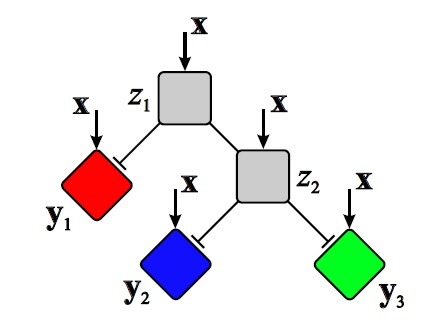
\includegraphics[scale = 0.5]{HME}
\caption{The graphical model of HME}\label{HME}
\end{figure}
\section{Continuous Latent Models}
\subsection{Principal component analysis}
The maximum variance formulation is equivalent to the minimum-error formulation. Now we consider the minimum-error formulation. We project the original data to a $M$-dimensional linear subspace. Suppose the $M$-dimensional subspace can be represented by the first $M$ of the basis vectors, and so we approximate each data $\bf{x}_n$ by
\begin{equation}
	\tilde{\bf{x}}_{n} = \sum_{i=1}^M z_{ni}\bf{u}_i  + \sum_{i=M+1}^D b_i \bf{u}_i
\end{equation}
where the $\{b_i \}$ are constants that are the same for all data points.

We shall use the squared distortion and our goal is to minimize
\begin{equation}
	J = \frac{1}{N} \sum_{n=1}^N ||\bf{x}_n-\tilde{\bf{x}}_n||^2.
\end{equation}

After some mathematical manipulations, we get that the general solution to the minimization of $J$ for arbitrary $D$ and arbitrary $M < D$ is obtained by choosing the $\{ \bf{u}_i \}$ to be eigenvectors of the covariance matrix given by
\begin{equation}
	\bf{S} \bf{u}_i = \lambda_i \bf{u}_i
\end{equation}
where $i=1,\cdots,D$, and as usual the eigenvectors $\{ \bf{u}_i \}$ are chosen to be orthonormal. In addition, we define
\begin{equation}
	 \bf{S} = \frac{1}{N} \sum_{n=1}^N (\bf{x}_n-\bar{\bf{x}})(\bf{x}_n-\bar{\bf{x}})^{\intercal}.
\end{equation}
The corresponding value of the distortion measure is then given by
\begin{equation}
	J = \sum_{i=M+1}^D \lambda_i.
\end{equation}
We therefore obtain the minimum value of $J$ by selecting these eigenvectors to be those having the $D-M$ smallest eigenvalues, and hence the eigenvectors defining the principal subspace are those corresponding to the $M$ \textbf{largest} eigenvalues.

After getting the eigenvectors $\{ \bf{u}_i \}$, the original data can be approximated by
\begin{align}
	\tilde{\bf{x}}_n = \bar{\bf{x}} + \sum_{i=1}^M (\bf{x}_n^{\intercal} \bf{u}_i - \bar{\bf{x}}^{\intercal} \bf{u}_i)\bf{u}_i
\end{align}

\subsection{Whitening}
Another name for the method is called \imp{sphereing}. This is a substantial normalization of the data to give it \textbf{zero mean} and \textbf{unit covariance}, inspired by PCA. To do this, we first diagonalize the data covariance $\bf{S}$ to give
\begin{equation}
	\bf{SU} = \bf{UL}.
\end{equation}
Then we define, for each data point $\bf{x}_n$, a transformed value given by
\begin{equation}
	\bf{y}_n = \bf{L}^{1/2}\bf{U}^{\intercal} (\bf{x}_n - \bar{\bf{x}}).
\end{equation}
\subsection{PCA for high-dimensional data}
This is a mathematical equivalent method to PCA but more efficient in \textbf{high-dimensional} case where $N < D$. First, we define $\bf{X}$ as the $(N \times D)$-dimensional centered data matrix, whose $n^{\up{th}}$ row is given by $(\bf{x}_n-\bar{\bf{x}})^{\intercal}$. The covariance matrix can then be written as $\bf{S} = N^{-1} \bf{X}^{\intercal} \bf{X}$, and the corresponding eigenvector equation becomes
\begin{equation}
	\frac{1}{N} \bf{X}^{\intercal} \bf{X}\bf{u}_i = \lambda_i \bf{u}_i.
\end{equation}
Now pre-multiply both sides by $\bf{X}$ to give
\begin{align}
	\frac{1}{N} \bf{XX}^{\intercal} (\bf{Xu}_i) &= \lambda_i (\bf{Xu}_i) \\
	\frac{1}{N} \bf{XX}^{\intercal} \bf{v}_i &= \lambda_i \bf{v}_i \label{HDPCA}
\end{align}
where $\bf{v}_i$ can be efficiently calculated in $O(N^3)$. Multiply both sides of (\ref{HDPCA}) by $\bf{X}^{\intercal}$ to give
\begin{equation}
	\left( \frac{1}{N} \bf{X}^{\intercal}\bf{X} \right)(\bf{X}^{\intercal} \bf{v}_i) = \lambda_i (\bf{X}^{\intercal} \bf{v}_i).
\end{equation}
Assuming $\bf{v}_i$ has been \textbf{normalized} to unit length, we get
\begin{equation}
	\bf{u}_i = \frac{1}{(N\lambda_i)^{1/2}} \bf{X}^{\intercal} \bf{v}_i.
\end{equation}
\subsection{Probabilistic PCA}
\subsubsection{Model}
The prior over $\bf{z}$ is given by (a more general Gaussian only leads to the same probabilistic model)
\begin{equation}
	p(\bf{z}) = \cal{N}(\bf{z}|\bf{0},\bf{I}).
\end{equation}
The conditional distribution of the observed variable $\bf{x}$ is given by
\begin{equation}
	p(\bf{x|z}) = \cal{N}(\bf{x}|\bf{Wz}+\bs{\mu},\sigma^2\bf{I}).
\end{equation}
where $\bf{W}$ is a $D \times M$ matrix. Note that this factorizes with respect to the elements of $\bf{x}$ and is hence an example of the \textbf{naive Bayes model}.

The marginal distribution over $\bf{x}$ and the conditional distribution of $\bf{z}$ given $\bf{x}$ can be obtained from formulae for linear-Gaussian model and are given by
\begin{align}
	p(\bf{x}) &= \cal{N}(\bf{x}|\bs{\mu},\bf{C}) \\
	p(\bf{z|x}) &= \cal{N}(\bf{z}|\bf{M}^{-1}\bf{W}^{\intercal}(\bf{x}-\bs{\mu}),\sigma^2\bf{M}^{-1})
\end{align}
where
\begin{align}
	\bf{C} &= \bf{W}\bf{W}^{\intercal} + \sigma^2 \bf{I} \label{PCA1}\\
	\bf{M} &= \bf{W}^{\intercal} \bf{W} + \sigma^2 \bf{I}.
\end{align}
From (\ref{PCA1}) we know that this model is invariant to rotations in the latent space since $\bf{wR}^{\intercal}\bf{Rw}^{\intercal} = \bf{ww}^{\intercal}$.

In addition, the inverse of $\bf{C}$ can be evaluated efficiently using (\ref{ide1}):
\begin{equation}
	\bf{C}^{-1} = \sigma^{-2}\bf{I} - \sigma^{-2}\bf{W}(\bf{W}^{\intercal}\bf{W}+\sigma^2 \bf{I})^{-1} \bf{W}^{\intercal}.
\end{equation}
\subsubsection{MLE method}
The log likelihood function is given by
\begin{equation}
	\ln p(\bf{X}|\bs{\mu},\bf{W},\sigma^2) = \frac{-ND}{2}\ln(2\pi)-\frac{N}{2}\ln|\bf{C}|-\frac{1}{2}\sum_{n=1}^N (\bf{x}_n-\bs{\mu})^{\intercal} \bf{C}^{-1} (\bf{x}_n - \bs{\mu}).
\end{equation}
Setting the derivatives with respect to $\bs{\mu}$, $\bf{W}$ and $\sigma^2$ to zero, we obtain
\begin{align}
	\bf{\mu} &= \bar{\bf{x}} \\
	\bf{W}_{ML} &= \bf{U}_M (\bf{L}_M-\sigma^2 \bf{I})^{1/2}\bf{R} \\
	\sigma_{ML}^2 &= \frac{1}{D-M} \sum_{i=M+1}^D \lambda_i
\end{align}
\subsubsection{EM for PCA}
The complete-data log likelihood function takes the form
\begin{equation}
	\ln p(\bf{X,Z}|\bs{\mu},\bf{W},\sigma^2) = \sum_{n=1}^N \{ \ln p(\bf{x}_n|\bf{z}_n)+ \ln p(\bf{z}_n) \}
\end{equation}

\textbf{The E step}. \begin{align}
\bb{E}[\ln p(\bf{X,Z}|\bs{\mu},\bf{W},\sigma^2)] = -\sum_{n=1}^N \{ \frac{D}{2}\ln (2\pi\sigma^2)+\frac{1}{2}\up{Tr}(\bb{E}[\bf{z}_n\bf{z}_n^{\intercal}])\\ +\frac{1}{2\sigma^2}||\bf{x}_n-\bs{\mu}||^2-\frac{1}{\sigma^2}\bb{E}[\bf{z}_n]^{\intercal} \bf{W}^{\intercal}(\bf{x}_n-\bs{\mu})\\+\frac{M}{2}\ln (2\pi)+\frac{1}{2\sigma^2}\up{Tr}(\bb{E}[\bf{z}_n\bf{z}_n^{\intercal}]\bf{W}^{\intercal}\bf{W}) \}
\end{align}
We use the old parameter values to evaluate
\begin{align}
	\bb{E}[\bf{z}_n] &= \bf{M}^{-1} \bf{W}^{\intercal} (\bf{x}_n-\bar{\bf{x}}) \label{PCAE1}\\
	\bb{E}[\bf{z}_n\bf{z}_n^{\intercal}] &= \sigma^2 \bf{M}^{-1} + \bb{E}[\bf{z}_n] \bb{E}[\bf{z}_n]^{\intercal}. \label{PCAE2}
\end{align}

\textbf{The M step}. We maximize with respect to $\bf{W}$ and $\sigma^2$, keeping the posterior statistics fixed. The M-step equations are
\begin{align}
	\bf{W}_{new} &= \left[ \sum_{n=1}^N (\bf{x}_n-\bar{\bf{x}})\bb{E}[\bf{z}_n]^{\intercal} \right]\left[
	\sum_{n=1}^N \bb{E}[\bf{z}_n\bf{z}_n^{\intercal}]\right]^{-1} \\
	\sigma_{new}^2 &= \frac{1}{ND} \sum_{n=1}^N \{ ||\bf{x}_n-\bar{\bf{x}}||^2 - 2\bb{E}[\bf{z}_n]^{\intercal} \bf{W}_{new}^{\intercal}(\bf{x}_n-\bar{\bf{x}})\\
	&\quad + \up{Tr}(\bb{E}[\bf{z}_n\bf{z}_n^{\intercal}]\bf{W}_{new}^{\intercal}\bf{W}_{new}) \}.\label{PCAM1}
\end{align}

The advantage of EM algorithm is the computational efficiency for \textbf{large-scale} applications. Compared to conventional PCA whose computational cost scales like $O(ND^2)$, the computationally demanding steps for EM is $O(NDM)$. As a result, EM will outperform conventional PCA in the case that $M\ll D$.

We can take the limit $\sigma^2 \rightarrow 0$ to obtain a valid EM-like algorithm for \textbf{standard PCA}. For simplicity, we define $\tilde{\bf{X}}$ to be a matrix of size $N \times D$ whose $n^{\up{th}}$ row is given by the vector $\bf{x}_n - \bar{\bf{x}}$ and similarly define $\bs{\Omega}$ to be a matrix of size $M \times N$ whose $n^{\up{th}}$ row is given by the vector $\bb{E}[\bf{z}_n]$. The E step of the EM algorithm for PCA then becomes
\begin{equation}
	\bs{\Omega} = (\bf{W}_{old}^{\intercal} \bf{W}_{old})^{-1}\bf{W}_{old}^{\intercal} \tilde{\bf{X}}^{\intercal}
\end{equation}
and the M step takes the form
\begin{equation}
	\bf{W}_{new} = \tilde{\bf{X}}^{\intercal} \bs{\Omega}^{\intercal} (\bs{\Omega}\bs{\Omega}^{\intercal})^{-1}.
\end{equation}
\subsubsection{Bayesian PCA and ARD}
The problem comes when we want to determine a suitable $M$ for PCA. If the eigenvalues of the covariance naturally form two groups, we can get $M$ simply by inspection. 

Another approach is to use \textbf{cross-validation} since the probabilistic PCA has a well-defined \textbf{likelihood} function. However, this approach is computational costly.

The third approach is Bayesian based on the evidence approximation. It involves a specific choice of prior over $\bf{W}$ that allows surplus dimensions in the principal subspace to be pruned out of the model. This corresponds to an example of \textbf{automatic relevance determination}, or \textbf{ARD}. Specifically, we define an independent Gaussian prior over each column of $\bf{W}$. Each Gaussian has an independent variance governed by a precision hyperparameter $\alpha_i$ so that
\begin{equation}
	p(\bf{W}|\bs{\alpha}) = \prod_{i=1}^M \left( \frac{\alpha_i}{2\pi} \right)^{D/2} \exp\left\{ -\frac{1}{2}\alpha_i \bf{w}_i^{\intercal} \bf{w}_i \right\}
\end{equation}
where $\bf{w}_i$ is the $i^{\up{th}}$ column of $\bf{W}$.

The marginal likelihood is given by
\begin{equation}
	p(\bf{X}|\bs{\alpha,\mu},\sigma^2) = \int p(\bf{X|W},\bs{\mu},\sigma^2) p(\bf{W}|\bs{\alpha}) \ud \bf{W}.
\end{equation}
We them make use of the Laplace approximation to evaluate this integral under the assumption that the posterior distribution is sharply peeked, as will occur for sufficiently \textbf{large} data sets. By analogy to what we discussed in Section \ref{DEigens}, the marginal likelihood with respect to $\alpha_i$ take the simple form
\begin{equation}
	\alpha_i^{new} = \frac{D}{\bf{w^*}_i^{\intercal} \bf{w^*}_i}
\end{equation}

As a result, we need to evaluate the \textbf{optimal} $\bf{W}^*$ in every \textbf{iteration}. This can been achieved by a variant of EM algorithm specially \textbf{modified} to evaluate MAP results. The re-estimation of $\alpha_i$ and $\bf{W}$ are \textbf{interleaved} with each other. The E-step equations are again given by (\ref{PCAE1}) and (\ref{PCAE2}). However, since the EM has been modified for MAP results, the M-step should be changed correspondingly. The M-step equation for $\sigma^2$ is again given by (\ref{PCAM1}). But the M-step equation for $\bf{W}$ is modified to give
\begin{equation}
	\bf{W}_{new} = \left[ \sum_{n=1}^N (\bf{x}_n-\bar{\bf{x}})\bb{E}[\bf{z}_n]^{\intercal} \right] \left[ \sum_{n=1}^N \bb{E}[\bf{z}_n\bf{z}_n^{\intercal}] +\sigma^2 \bf{A}\right]^{-1}
\end{equation}
where $\bf{A} = \up{diag}(\alpha_i)$. The value of $\bs{\mu}$ is given by the sample mean as before.

\subsection{Factor analysis}
The only difference in Factor analysis compared to probabilistic PCA is that the conditional distribution of the observed variable $\bf{x}$ given the latent variable $\bf{z}$ is taken to have a diagonal rather than an isotropic covariance so that
\begin{equation}
	p(\bf{x|z}) = \cal{N} (\bf{x}|\bf{Wz}+\bs{\mu},\bs{\Psi})
\end{equation}
where $\bs{\Psi}$ is a $D \times D$ diagonal matrix. 

In the factor analysis literature, the columns of $\bf{W}$, which capture the correlations between observed variables, are called \imp{factor loadings}, and the diagonal elements of $\bs{\Psi}$, which represent the independent noise variances for each of the variables, are called \imp{uniquenesses}.

There is no closed-form maximum likelihood solution for $\bf{W}$ in factor analysis, so we have to turn to EM. The iteration equations are similar to those in probabilistic PCA.
\subsection{Kernel PCA}
\textbf{Motivation}. Usually we can take an algorithm expressed in terms of \textbf{scalar products} of the form $\bf{x}^{\intercal} \bf{x'}$ and generalize that algorithm by replacing the scalar products with a nonlinear kernel. We will do the same thing for standard PCA and get a nonlinear generalization called \imp{kernel PCA}.

First suppose that we have \textbf{subtracted the sample mean} from each of the vectors $\bf{x}_n$ and recall that the principal components are defined by the normalized eigenvectors $\bf{u}_i$ of the covariance matrix
\begin{equation}
	\bf{Su}_i = \frac{1}{N} \sum_{n=1}^N \bf{x}_n\bf{x}_n^{\intercal} = \lambda_i \bf{u}_i
\end{equation}

Now consider a nonlinear transformation $\bs{\phi}(\bf{x})$ into an $M$-dimensional feature space, so that each data point $\bf{x}_n$ is thereby projected onto a point $\bs{\phi}(\bf{x}_n)$. We can now perform standard PCA in the feature space analogously:
\begin{equation}
	\bf{Cv}_i = \frac{1}{N}\sum_{n=1}^N \bs{\phi}(\bf{x}_n)\bs{\phi}(\bf{x}_n)^{\intercal} \bf{v}_i = \lambda_i \bf{v}_i \label{KPCA1}
\end{equation}
where we surly have temporarily assumed that the projected data set also has \textbf{zero mean} for simplicity. Once having solved these eigenvalues and eigenvectors, the projection of a point $\bf{x}$ onto eigenvector $i$ is given by
\begin{equation}
	y_i(\bf{x}) = \bs{\phi}(\bf{x})^{\intercal} \bf{v}_i
\end{equation}

However, we must not forget that one of the most important aims for kernel methods is to avoid direct manipulations in feature space. So we must solve this problem without having to work \textbf{explicitly} in the feature space.

\textbf{Derivation}.  From (\ref{KPCA1}) we find $\bf{v}_i$ can be written in a linear combination of the $\bs{\phi}(\bf{x}_n)$, i.e.
\begin{equation}
	\bf{v}_i = \sum_{n=1}^N a_{in}\bs{\phi}(\bf{x}_n).
\end{equation}
As a result, the projection of $\bf{x}$ can be given in a kernel form by
\begin{equation}
	y_i(\bf{x}) = \sum_{n=1}^N a_{in}\bs{\phi}(\bf{x})^{\intercal} \bs{\phi}(\bf{x}_n) = \sum_{n=1}^N a_{in} k(\bf{x},\bf{x}_n).
\end{equation}
Substitute the expansion of $\bf{v}_i$ into the eigenvector equation (\ref{KPCA1}), we obtain
\begin{equation}
	\frac{1}{N} \sum_{n=1}^N \bs{\phi}(\bf{x}_n)\bs{\phi}(\bf{x}_n)^{\intercal} \sum_{m=1}^N a_{im} \bs{\phi}(\bf{x}_m)=\lambda_i\sum_{n=1}^N a_{in}\bs{\phi}(\bf{x}_n).
\end{equation}
The key step now is to express this eigenvector equation in terms of $\bf{a}_i$ in a \textbf{kernel} form. Multiply both sides by $\bs{\phi}(\bf{x}_l)^{\intercal}$ to give
\begin{equation}
	\bf{K}^2 \bf{a}_i = \lambda_i N \bf{Ka}_i
\end{equation}
This can be proved to be equivalent to
\begin{equation}
	\bf{Ka}_i = \lambda_i N \bf{a}_i
\end{equation}
for the purpose of predictions. One more thing to do is to normalize $\bf{v}_i$, which can be done in the form of $\bf{a}_i$ by
\begin{equation}
	1 = \bf{v}_i^{\intercal} \bf{v}_i = \bf{a}_i^{\intercal} \bf{Ka}_i = \lambda_i N \bf{a}_i^{\intercal}\bf{a}_i.
\end{equation}

Now we handle the problem of non-zero means of $\bs{\phi}(\bf{x}_n)$. The projected data points after \textbf{centralizing} are given by
\begin{equation}
	\tilde{\bs{\phi}}(\bf{x}_n) = \bs{\phi}(\bf{x}_n) - \frac{1}{N} \sum_{l=1}^N \bs{\phi}(\bf{x}_l)
\end{equation}
and the corresponding elements of the Gram matrix are given by
\begin{align}
	\tilde{\bf{K}} = \bf{K} - \bf{1}_N\bf{K} - \bf{K} \bf{1}_N + \bf{1}_N \bf{K} \bf{1}_N
\end{align}
where $\bf{1}_N$ denotes the $N \times N$ matrix in which every element takes the value $1/N$. After having established the relationship between $\tilde{\bf{K}}$ and $\bf{K}$, the more generalized problem is solved by direct analogy.

However, kernel PCA cannot be applied to data compression directly due to the following reason. Note that the mapping $\bs{\phi}(\bf{x})$ maps the $D$-dimensional $\bf{x}$ space into a $D$-dimensional manifold in the $M$-dimensional feature space. The vector $\bf{x}$ is known as the \imp{pre-image} of the corresponding point $\bf{\phi}(\bf{x})$. However, the projection of points in feature space onto the linear PCA subspace in that space will typically not lie on the nonlinear $D$-dimensional manifold and so \textbf{will not have a corresponding pre-image in data space}. Approximation techniques are needed.

\subsection{Independent component analysis (ICA)}
This is a model in which the observed variables are related linearly to the latent variables, but for which the latent distribution is non-Gaussian. Furthermore, the joint distribution of latent variables factorizes.
\subsection{Autoassociative neural networks}
This is a multilayer perceptron having $D$ inputs, $D$ output units and $M$ hidden units with $M < D$, as shown in Figure \ref{ANN}.
\begin{figure}
	\centering
	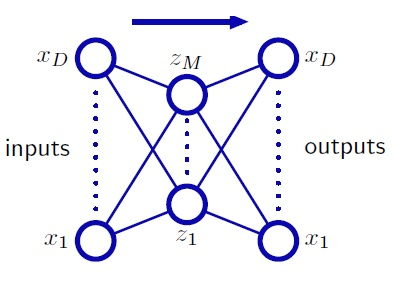
\includegraphics[scale=0.5]{ANN}
	\caption{Autoassociative Multilayer Perpceptron} \label{ANN}
\end{figure}

We therefore determine the network parameters $\bf{w}$ by minimizing an error function which captures the degree of mismatch between the input vectors and their reconstructions. Particularly, we can choose
\begin{equation}
E(\bf{w}) = \frac{1}{2} \sum_{n=1}^N ||\bf{y}(\bf{x}_n,\bf{w})-\bf{x}_n||^2.
\end{equation}

However, such a network can be proved to give same results as those of standard PCA, despite nonlinear activation functions. In order to model nonlinear PCA, we need to add additional hidden layers, which is shown by Figure \ref{ANN2}.
\begin{figure}
	\centering
	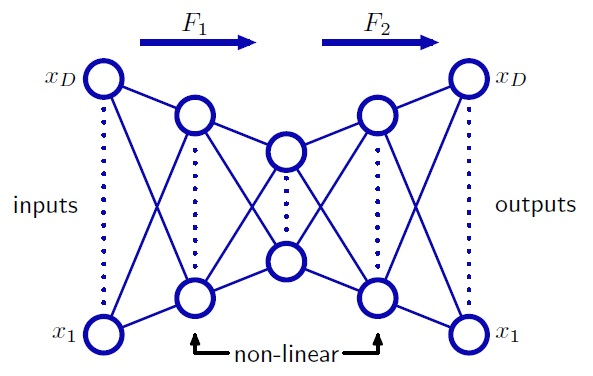
\includegraphics[scale = .4]{ANN2}
	\caption{Nonlinear PCA} \label{ANN2}
\end{figure}
Again the outputs units are linear and the $M$ units in the \textbf{second} hidden layer can also be linear, however, the \textbf{first} and \textbf{third} hidden layers have sigmoidal nonlinear activation functions. This model can be viewed as two successive functional mappings.
\section{Sequential Models}
\subsection{Hidden Markov models (HMM)}
The graphical model for HMM is shown by Figure \ref{HMM}.
\begin{figure}
	\centering
	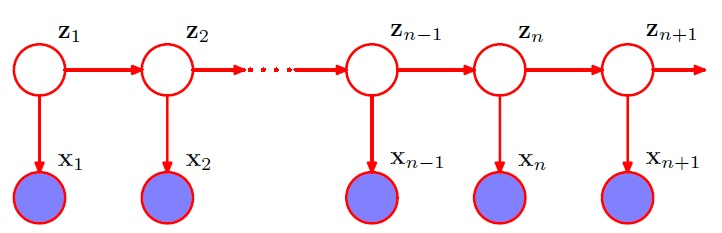
\includegraphics[scale=.5]{HMM}
	\caption{Markov Chain of Latent Variables Model}\label{HMM}
\end{figure}

As in the case of a standard mixture model, the latent variables are the discrete \textbf{multinomial} variables $\bf{z}_n$ describing which component of the mixture is responsible for generating the corresponding observation $\bf{x}_n$. 

\subsubsection{Latent variables}
For the Markov chain, we define the transition matrix $\bf{A}$ by $A_{jk} = p(z_{nk}=1|z_{n-1,j}=1)$. We can then write the conditional distribution explicitly in the form
\begin{equation}
	p(\bf{z}_n|\bf{z}_{n-1},\bf{A}) = \prod_{k=1}^K \prod_{j=1}^K A_{jk}^{z_{n-1,j}z_{nk}}.
\end{equation}
The initial latent node $\bf{z}_1$ is special in that it does not have a parent node, so that
\begin{equation}
	p(\bf{z}_1|\bs{\pi}) = \prod_{k=1}^K \pi_k^{z_{1k}}.
\end{equation}

Here we mention a special variant of the standard HMM model called \imp{left-to-right} HMM, which is obtained by setting the elements $A_{jk}$ of $\bf{A}$ to zero if $k<j$. Every such sequence is constrained to start in state $j=1$.
\subsubsection{Observed variables}
We can represent the \imp{emission probabilities} in the form
\begin{equation}
	p(\bf{x}_n|\bf{z}_n,\bs{\phi}) = \prod_{k=1}^K p(\bf{x}_n|\bs{\phi}_k)^{z_{nk}}.
\end{equation}

The joint probability distribution over both latent and observed variables is the given by
\begin{equation}
	p(\bf{X,Z}|\bs{\theta}) = p(\bf{z}_1|\bs{\pi})\left[\prod_{n=2}^N p(\bf{z}_n|\bf{z}_{n-1},\bf{A})\right] \prod_{m=1}^N p(\bf{x}_m|\bf{z}_m,\bs{\phi}).
\end{equation}
where $\bs{\theta}=\{ \bs{\pi},\bf{A},\bs{\phi} \}$ denotes the set of parameters governing the model.

\subsubsection{Likelihood}
Marginalizing over the latent variables, we obtain the likelihood of HMM:
\begin{equation}
	p(\bf{X}|\bs{\theta}) = \sum_{\bf{Z}} p(\bf{X,Z}|\bs{\theta}).
\end{equation}

We turn to the EM algorithm to find an efficient framework for maximizing the likelihood function in hidden Markov models. 

\subsubsection{E step}
We first introduce some convenient notations:
\begin{align}
	\gamma(\bf{z}_n) &= p(\bf{z}_n|\bf{X},\bs{\theta}^{old}) \\
	\xi(\bf{z}_{n-1},\bf{z}_n) &= p(\bf{z}_{n-1},\bf{z}_n|\bf{X},\bs{\theta}^{old}).
\end{align}
Note that we have
\begin{align}
	\gamma(z_{nk}) &= \bb{E}[z_{nk}] \\
	\xi(z_{n-1,j},z_{nk}) &= \bb{E}[z_{n-1,j}z_{nk}].
\end{align}

The expectation is given by
\begin{align}
	Q(\bs{\theta,\theta}^{old}) = &\sum_{k=1}^K \gamma(z_{1k}) \ln \pi_k +\sum_{n=2}^N \sum_{j=1}^K \sum_{k=1}^K \xi(z_{n-1,j},z_{nk})\ln A_{jk} \\
	&+\sum_{n=1}^N \sum_{k=1}^K \gamma(z_{nk}) \ln p(\bf{x}_n|\bs{\phi}_k).
\end{align}

The goal of the E step will be to evaluate the quantities $\gamma(\bf{z}_n)$ and $\xi(\bf{z}_{n-1},\bf{z}_n)$ efficiently, where \textbf{sum-product algorithm} is used.

First, we need to get the equivalent factor graph for HMM. For the purpose of solving the inference problem, we can always simplify the factor graph by absorbing the emission probabilities into the transition probability factors since we need to condition on the observed variables. This leads to the simplified factor graph representation in Figure \ref{HMMFG}, in which the factors are given by
\begin{align}
	h(\bf{z}_1) &= p(\bf{z}_1)p(\bf{x}_1|\bf{z}_1) \\
	f_n(\bf{z}_{n-1},\bf{z}_n) &= p(\bf{z}_n|\bf{z}_{n-1})p(\bf{x}_n|\bf{z}_n).
\end{align}
\begin{figure}
	\centering
	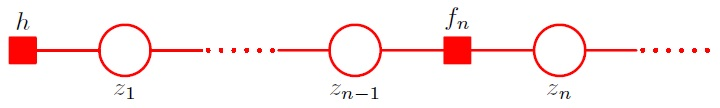
\includegraphics[scale=.5]{HMMFG}
	\caption{A simplified form of factor graph to describe the hidden Markov model.} \label{HMMFG}
\end{figure}

Now we denote the final hidden variable $\bf{z}_N$ as the root node, and first pass messages from the leaf node $h$ to the root. From what we have discussed in Section \ref{SumProd}, we have the propagation equations for the messages
\begin{align}
	\mu_{\bf{z}_{n-1}\rightarrow f_n}(\bf{z}_{n-1}) &= \mu_{f_{n-1}\rightarrow \bf{z}_{n-1}}(\bf{z}_{n-1}) \\
	\mu_{f_n \rightarrow \bf{z}_{n}}(\bf{z}_n) &= \sum_{\bf{z}_{n-1}}f_n (\bf{z}_{n-1},\bf{z}_n)\mu_{\bf{z}_{n-1}\rightarrow f_n}(\bf{z}_{n-1})
\end{align}
Then we define $\alpha(\bf{z}_n) = \mu_{f_n \rightarrow \bf{z}_n}(\bf{z}_n)$ and simplify the message propagation equation to get
\begin{align}
	\alpha(\bf{z}_n) &= \sum_{\bf{z}_{n-1}} f_n (\bf{z}_{n-1},\bf{z}_n) \alpha(\bf{z}_{n-1})\\
	\alpha(\bf{z}_1) &= p(\bf{z}_1)p(\bf{x}_1|\bf{z}_1)=\prod_{k=1}^K \{ \pi_k p(\bf{x}_1|\bs{\phi}_k) \}^{z_{1k}}.
\end{align}
Similarly we define $\beta(\bf{z}_n) = \mu_{f_{n+1}-\rightarrow\bf{z}_n}(\bf{z}_n)$ and derive the back propagation equation
\begin{align}
	\beta(\bf{z}_n) &= \sum_{\bf{z}_{n+1}} f(\bf{z}_n,\bf{z}_{n+1}) \beta(\bf{z}_{n+1}). \\
	\beta(\bf{z}_n) &= 1
\end{align}
The posterior distribution of each latent variable can then be written by
\begin{equation}
	\gamma(\bf{z}_n) = p(\bf{z}_n|\bf{X}) = \frac{p(\bf{X}|\bf{z}_n)p(\bf{z}_n)}{p(\bf{X})}
\end{equation}
and
\begin{align}
	\xi(\bf{z}_{n+1}|\bf{z}_n) &= \frac{p(\bf{X}|\bf{z}_{n-1},\bf{z}_n)p(\bf{z}_{n-1},\bf{z}_n)}{p(\bf{X})} \\
	&= \frac{\alpha(\bf{z}_{n-1})p(\bf{x}_n|\bf{z}_n)p(\bf{z}_n|\bf{z}_{n-1})\beta(\bf{z}_n)}{p(\bf{X})}.
\end{align}

However, this method has a severe flaw \textbf{numerically}. Because the probabilities are often significantly less than unity, as we work our way forward along the chain, the values of $\alpha(\bf{z}_n)$ can go to zero \textbf{exponentially} quickly. We try to define a normalized version of $\alpha$ given by
\begin{equation}
	\hat{\alpha}(\bf{z}_n) = p(\bf{z}_n|\bf{x}_1,\cdots,\bf{x}_n)=\frac{\alpha(\bf{z}_n)}{p(\bf{x}_1,\cdots,\bf{x}_n)}
\end{equation}
which we expect to be well behaved numerically because it is a probability distribution \textbf{over $K$ variables for any value of $n$.} Similarly, we introduce scaling factors defined by conditional distributions over the observed variables
\begin{equation}
	c_n = p(\bf{x}_n|\bf{x}_1,\cdots,\bf{x}_{n-1}).
\end{equation}
As a result,
\begin{equation}
	\alpha(\bf{z}_n) = \left( \prod_{m=1}^n c_m \right) \hat{\alpha}(\bf{z}_n).
\end{equation}
Then the recursion equation for $\alpha$ is given by
\begin{equation}
	c_n \hat{\alpha}(\bf{z}_n) = p(\bf{x}_n|\bf{z}_n)\sum_{\bf{z}_{n-1}} \hat{\alpha}(\bf{z}_{n-1})p(\bf{z}_n|\bf{z}_{n-1})
\end{equation}
and similarly
\begin{equation}
	c_{n+1}\hat{\beta}(\bf{z}_n) = \sum_{\bf{z}_{n+1}} \hat{\beta}(\bf{z}_{n+1})p(\bf{x}_{n+1}|\bf{z}_{n+1})p(\bf{z}_{n+1}|\bf{z}_n).
\end{equation}

The required marginals are given by
\begin{align}
	\gamma(\bf{z}_n) &= \hat{\alpha}(\bf{z}_n) \hat{\beta}(\bf{z}_n) \\
	\xi(\bf{z}_{n-1},\bf{z}_n) &= c_n^{-1} \hat{\alpha}(\bf{z}_{n-1})p(\bf{x}_n|\bf{z}_n)p(\bf{z}_n|\bf{z}_{n-1})\hat{\beta}(\bf{z}_n).
\end{align}

If we want to find the most probable sequence of hidden states for a given observation sequence, we can employ the back-tracing method discussed in Section \ref{MaxSum}, which is also called \imp{Viterbi algorithm} in the literature of HMM.

\subsubsection{M step}
We maximize $Q(\bs{\theta},\bs{\theta}^{old})$ with respect to the parameters $\bs{\theta}=\{\bs{\pi},\bf{A},\bs{\phi} \}$ in which we treat $\gamma(\bf{z}_n)$ and $\xi(\bf{z}_{n-1},\bf{z}_n)$ as constant. Using Lagrange multipliers we obtain
\begin{align}
	\pi_k &= \frac{\gamma(z_{1k})}{\sum_{j=1}^K \gamma(z_{1j})} \\
	A_{jk} &= \frac{\sum_{n=2}^N \xi(z_{n-1,j},z_{nk})}{\sum_{l=1}^K\sum_{n=2}^N \xi(z_{n-1,j},z_{nl})}.
\end{align}
Note that any elements of $\bs{\pi}$ or $\bf{A}$ that are set to zero \textbf{initially} will \textbf{remain zero} in subsequent EM updates.
\subsection{Linear dynamical systems (LDS)}
This is a model in which the latent variables $\{\bf{z}_n\}$ as well as the observed variables $\{\bf{x}_n\}$ are multivariate Gaussian distributions whose means are linear functions of the states of their parents in the graph. The graphical model for LDS is again shown in Figure \ref{HMM}. LDS can be viewed as a generalization of the continuous latent variable models such as probabilistic PCA and factor analysis. 

The transition and emission distributions are in the general form
\begin{align}
	p(\bf{z}_1) &= \cal{N}(\bf{z}_1|\bs{\mu}_0,\bf{V}_0)\\
	p(\bf{z}_n|\bf{z}_{n-1}) &= \cal{N}(\bf{z}_n|\bf{Az}_{n-1},\bs{\Gamma}) \\
	p(\bf{x}_n|\bf{z}_n) &= \cal{N}(\bf{x}_n|\bf{Cz}_{n},\bs{\Sigma}).
\end{align}
The model parameters are $\bs{\theta}=\{ \bf{A},\bs{\Gamma},\bf{C},\bs{\Sigma},\bs{\mu}_0,\bf{V}_0 \}$.
\subsubsection{E step}
We again define
\begin{equation}
	\hat{\alpha}(\bf{z}_n) = \cal{N}(\bf{z}_n|\bs{\mu}_n,\bf{V}_n)
\end{equation}
and the recursion equation takes the form by analogy
\begin{equation}
	c_n \hat{\alpha}(\bf{z}_n) = p(\bf{x}_n|\bf{z}_n)\int \hat{\alpha}(\bf{z}_{n-1})p(\bf{z}_n|\bf{z}_{n-1})\ud \bf{z}_{n-1}.
\end{equation}
Making use of the linear-Gaussian formulae, we obtain
\begin{align}
	c_n \cal{N}(\bf{z}_n|\bs{\mu}_n,\bf{V}_n) = \cal{N}(\bf{x}_n|\bf{Cz}_n,\bs{\Sigma})\cal{N}(\bf{z}_n|\bf{A}\bs{\mu}_{n-1},\bf{P}_{n-1})
\end{align}
where
\begin{equation}
	\bf{P}_{n-1} = \bf{AV}_{n-1}\bf{A}^{\intercal} + \bs{\Gamma}.
\end{equation}

Making use of the linear-Gaussian formulae again, we obtain
\begin{align}
	\bs{\mu}_n &= \bf{A} \bs{\mu}_{n-1} + \bf{K}_n (\bf{x}_n - \bf{CA}\bs{\mu}_{n-1}) \\
	\bf{V}_n &= (\bf{I}-\bf{K}_n \bf{C})\bf{P}_{n-1} \\
	c_n &= \cal{N}(\bf{x}_n|\bf{CA}\bs{\mu}_{n-1},\bf{CP}_{n-1}\bf{C}^{\intercal} + \bs{\Sigma}).
\end{align}
Here we have made use of the matrix inverse identities (\ref{ide0}) and (\ref{ide2}) and also defined the \imp{Kalman gain matrix}
\begin{equation}
	\bf{K}_n = \bf{P}_{n-1} \bf{C}^{\intercal}(\bf{CP}_{n-1}\bf{C}^{\intercal} + \bs{\Sigma})^{-1}.
\end{equation}
The initial conditions for these recursion equations are obtained from
\begin{equation}
	c_1\hat{\alpha}(\bf{z}_1) = p(\bf{z}_1)p(\bf{x}_1|\bf{z}_1)
\end{equation}
which can again be treated using linear-Gaussian formulae to obtain
\begin{align}
	\bs{\mu}_1 &= \bs{\mu}_0 + \bf{K}_1 (\bf{x}_1-\bf{C}\bs{\mu}_0) \\
	\bf{V}_1 &= (\bf{I}-\bf{K}_1\bf{C})\bf{V}_0 \\
	c_1 &= \cal{N}(\bf{x}_1|\bf{C}\bs{\mu}_0,\bf{CV}_0\bf{C}^{\intercal}+\bs{\Sigma})
\end{align}
where
\begin{equation}
	\bf{K}_1 = \bf{V}_0\bf{C}^{\intercal}(\bf{CV}_0\bf{C}^{\intercal}+\bs{\Sigma})^{-1}.
\end{equation}

In the LDS literature, it is usual to formulate this backward recursion in terms of $\gamma(\bf{z}_n) = p(\bf{z}_n|\bf{X})= \hat{\alpha}(\bf{z}_n)\hat{\beta}(\bf{z}_n)$ rather than in terms of $\hat{\beta}(\bf{z}_n)$. Because $\gamma(\bf{z}_n)$ must also be Gaussian, we write it in the form
\begin{equation}
	\gamma(\bf{z}_n) = \hat{\alpha}(\bf{z}_n)\hat{\beta}(\bf{z}_n)=\cal{N}(\bf{z}_n|\hat{\bs{\mu}}_n,\hat{\bf{V}}_n).
\end{equation}
The recursion equations for $\gamma$ can be obtained similarly to be
\begin{align}
	\hat{\bs{\mu}}_n &= \bs{\mu}_n + \bf{J}_n (\hat{\bs{\mu}}_{n+1}-\bf{A}\bs{\mu}_n) \\
	\hat{\bf{V}}_n &= \bf{V}_n + \bf{J}_n(\hat{\bf{V}}_{n+1}-\bf{P}_n)\bf{J}_n^{\intercal}
\end{align}
where we have defined
\begin{equation}
	\bf{J}_n = \bf{V}_n \bf{A}^{\intercal} (\bf{P}_n)^{-1}.
\end{equation}

For the EM algorithm, we also require the pairwise posterior marginals in the form
\begin{align}
	\xi(&\bf{z}_{n-1},\bf{z}_n) = (c_n)^{-1}\hat{\alpha}(\bf{z}_{n-1})p(\bf{x}_n|\bf{z}_n)p(\bf{z}_n|\bf{z}_{n-1})\hat{\beta}(\bf{z}_n) \\
	&=\frac{\cal{N}(\bf{z}_{n-1}|\bs{\mu}_{n-1},\bf{V}_{n-1})\cal{N}(\bf{z}_n|\bf{Az}_{n-1},\bs{\Gamma})\cal{N}(\bf{x}_n|\bf{Cz}_n,\bs{\Sigma})\cal{N}(\bf{z}_n|\hat{\bs{\mu}}_n,\hat{\bf{V}}_n)}{c_n\hat{\alpha}(\bf{z}_n)}
\end{align}
\subsubsection{M step}
The following expectations are required in the M step:
\begin{align}
	\bb{E}[\bf{z}_n] &= \hat{\bs{\mu}}_n \\
	\bb{E}[\bf{z}_n\bf{z}_{n-1}^{\intercal}] &= \hat{\bf{V}}_n \bf{J}_{n-1}^{\intercal} +\hat{\bs{\mu}}_n\hat{\bs{\mu}}_{n-1}^{\intercal}\\
	\bb{E}[\bf{z}_n\bf{z}_n^{\intercal}] &= \hat{\bf{V}}_n + \hat{\bs{\mu}}_n \hat{\bs{\mu}}_n^{\intercal}
\end{align}
Then we maximize $Q(\bs{\theta},\bs{\theta}^{old}) = \bb{E}_{\bf{Z}|\bs{\theta}^{old}}[\ln p(\bf{X,Z}|\bs{\theta})]$ with respect to the parameters alternatively.

For $\bs{\mu}_0$ and $\bf{V}_0$, we have
\begin{align}
	\bs{\mu}_0^{new} &= \bb{E}[\bf{z}_1] \\
	\bf{V}_0^{new} &= \bb{E}[\bf{z}_1\bf{z}_1^{\intercal}] - \bb{E}[\bf{z}_1]\bb{E}[\bf{z}_1^{\intercal}].
\end{align}

For $\bf{A}$ and $\bs{\Gamma}$, we obtain
\begin{align}
	\bf{A}^{new} &= \left(\sum_{n=2}^N \bb{E}[\bf{z}_n \bf{z}_{n-1}^{\intercal}]\right)\left( \sum_{n=2}^N \bb{E}[\bf{z}_{n-1}\bf{z}_{n-1}^{\intercal}] \right)^{-1} \\
	\bs{\Gamma}^{new} &= \frac{1}{N-1} \sum_{n=2}^N \{ \bb{E}[\bf{z}_n\bf{z}_n^{\intercal}]-\bf{A}^{new}\bb{E}[\bf{z}_{n-1}\bf{z}_n^{\intercal}] \notag\\
	-&\bb{E}[\bf{z}_n\bf{z}_{n-1}^{\intercal}](\bf{A}^{new})^{\intercal} + \bf{A}^{new} \bb{E}[\bf{z}_{n-1}\bf{z}_{n-1}^{\intercal}] (\bf{A}^{new})^{\intercal}\}.
\end{align}

Finally, for $\bf{C}$ and $\bs{\Sigma}$, we have
\begin{align}
	\bf{C}^{new} &= \left( \sum_{n=1}^N \bf{x}_n \bb{E}[\bf{z}_n^{\intercal}] \right)\left( \sum_{n=1}^N \bb{E}[\bf{z}_n\bf{z}_n^{\intercal}] \right)^{-1} \\
	\bs{\Sigma}^{new} &= \frac{1}{N} \sum_{n=1}^N \{ \bf{x}_n\bf{x}_n^{\intercal} -\bf{C}^{new}\bb{E}[\bf{z}_n]\bf{x}_n^{\intercal} \notag \\
	&\quad - \bf{x}_n \bb{E}[\bf{z}_n^{\intercal}](\bf{C}^{new})^{\intercal} + \bf{C}^{new}\bb{E}[\bf{z}_n\bf{z}_n^{\intercal}](\bf{C}^{new})^{\intercal}\}.		 
\end{align}
\subsection{Particle filters}
For dynamical systems which do not have a linear-Gaussian, we can turn to \textbf{sampling methods} in order to find a tractable inference algorithm. In particular, we can apply the sampling-importance-resampling formalism to obtain a sequential Monte Carlo algorithm known as the \imp{particle filter}, which also has other names such as \imp{bootstrap filter}, \imp{survival of the fittest} and the \imp{condensation} algorithm.

The graphical model for particle filters is also represented in Figure \ref{HMM}. 

\subsubsection{E step}
Suppose we are given the observed values $\bf{X}_n = (\bf{x}_1,\cdots,\bf{x}_n)$ and we wish to draw $L$ samples from the posterior distribution $p(\bf{z}_n|\bf{X}_n)$. Using Bayes' theorem, we have
\begin{align}
	\bb{E}[f(\bf{z}_n)] &= \int f(\bf{z}_n)p(\bf{z}_n|\bf{X}_n) \ud \bf{z}_n \notag\\
	&= \frac{\int f(\bf{z}_n)p(\bf{x}_n|\bf{z}_n)p(\bf{z}_n|\bf{X}_{n-1})\ud \bf{z}_n}{\int p(\bf{x}_n|\bf{z}_n)p(\bf{z}_n|\bf{X}_{n-1})\ud \bf{z}_n} \notag\\
	&\simeq \sum_{l=1}^L w_n^{(l)} f(\bf{z}_n^{(l)}) \label{PF1}
\end{align}
where $\{ \bf{z}_n^{(l)}\}$ is a set of samples drawn from $p(\bf{z}_n|\bf{X}_{n-1})$ and the sampling weights $\{ w_n^{(l)} \}$ are defined by
\begin{equation}
	w_n^{(l)} = \frac{p(\bf{x}_n|\bf{z}_n^{(l)})}{\sum_{m=1}^L p(\bf{x}_n|\bf{z}_n^{(m)})}.
\end{equation}

We wish to find a sequential sampling scheme. We shall suppose that a set of samples and weights have been obtained at time step $n$, and that we have subsequently observed the value of $\bf{x}_{n+1}$, and we wish to find the weights and samples at time step $n+1$. We first sample from $p(\bf{z}_{n+1}|\bf{X}_n)$. This is again obtained using Bayes' theorem
\begin{align}
	p(\bf{z}_{n+1}|\bf{X}_n) &= \int p(\bf{z}_{n+1}|\bf{z}_n,\bf{X}_n)p(\bf{z}_n|\bf{X}_n)\ud \bf{z}_n \notag\\
	&=\frac{\int p(\bf{z}_{n+1}|\bf{z}_n)p(\bf{x}_n|\bf{z}_n)p(\bf{z}_n|\bf{X}_{n-1})\ud \bf{z}_n}{\int p(\bf{x}_n|\bf{z}_n)p(\bf{z}_n|\bf{X}_{n-1})\ud \bf{z}_{n-1}}\notag\\
	&\simeq \sum_l w_n^{(l)} p(\bf{z}_{n+1}|\bf{z}_n^{(l)}) \label{PF2}
\end{align}
This is a mixture distribution, and samples can be drawn by choosing a component $l$ with probability given by the mixing coefficients $w^{(l)}$ and then drawing a sample from the corresponding component.

In summary, each step of the particle filter algorithm comprises two stages. At time step $n$, we have a set of samples from $p(\bf{z}_n|\bf{X}_n)$. Then we use (\ref{PF2}) to get samples from $p(\bf{z}_{n+1}|\bf{X}_n)$. After getting $\bf{x}_{n+1}$, we employ (\ref{PF1}) to compute the posterior expectation and simultaneously apply samping-importance-resampling scheme to obtain new samples from $p(\bf{z}_{n+1}|\bf{X}_{n+1})$.
\end{document}
